% Modified for use with IJQC - Madhusudan Singh Copyright (C) (2011). All rights reserved.
\documentclass[12pt]{article}

\setlength{\oddsidemargin}{0in}  %left margin position, reference is one inch
\setlength{\textwidth}{6.5in}    %width of text=8.5-1in-1in for margin
\setlength{\topmargin}{-0.5in}    %reference is at 1.5in, -.5in gives a start of about 1in from top
\setlength{\textheight}{9in}     %length of text=11in-1in-1in (top and bot. marg.) 


\usepackage{amsmath,amssymb}
\usepackage{graphicx}% Include figure files
\usepackage{caption}
\usepackage{color}% Include colors for document elements
\usepackage{dcolumn}% Align table columns on decimal point
\usepackage{bm}% bold math
\usepackage[numbers,super,comma,sort&compress]{natbib}
%\usepackage[nolists, nomarkers, figuresfirst]{endfloat}

\usepackage{soul}

\definecolor{background-color}{gray}{0.98}
\graphicspath{{data/}{images/}}

%\title{Atomic pseudo-potentials for sp$^2$ carbon atoms}
\title{Atomic pseudo-potentials for reproducing the valence electron behaviour of sp$^2$ carbon atoms}
\author{Alexander Punter\thanks{Aix Marseille Univ, CNRS, Centrale Marseille, iSm2, Marseille, France}, Paola Nava\thanks{Aix Marseille Univ, CNRS, Centrale Marseille, iSm2, Marseille, France}, Yannick Carissan \thanks{Aix Marseille Univ, CNRS, Centrale Marseille, iSm2, Marseille, France}}

\begin{document}

\maketitle


\begin{abstract}
A pseudo-potential system for recreating an sp\(^{2}\) carbon atom is built 
and tested as a building block for various pseudo-hydrocarbon chain and ring systems.  
This pseudo-system has a central charge of 1, thus it contains only one
electron. It is employed in \textsl{ab-initio} calculations in which several physical characterstics
including first ionisation and excitation energies, as well as the HOMO energy, 
are found to be well-reproduced by the pseudo-system.
\end{abstract}

\clearpage

  \makeatletter
  \renewcommand\@biblabel[1]{#1.}
  \makeatother

\bibliographystyle{apsrev}

\renewcommand{\baselinestretch}{1.5}
\normalsize


\clearpage

%%BEGTXT
\section*{\sffamily \Large INTRODUCTION}

It is a common idea that a chemical system can be thought of as comprised of (at least) 
two parts:
an active one, where most of the chemistry takes place, and an (apparently) inactive
one, which must be taken into account in order to fulfill chemical requirements.
Based on this general statement, many successful theoretical approaches have been developed.
Among them can be cited QM/QM' or QM/MM methods, where 
the active region that usually contains several atoms is
treated at a high level of calculation, while the inactive part is treated at a 
lower level of theory.\cite{chung_oniom_2015,
ihrig_specific_2011,
zhang_pseudobond_1998,
dilabio_simple_2002,
dilabio_efficient_2005,
gao_generalized_1998,
assfeld_quantum_1996,
jacob_calculation_2006,
von_lilienfeld_variational_2004,
von_lilienfeld_performance_2005,
von_lilienfeld_optimization_2004,
goedecker_separable_1996,
hartwigsen_relativistic_1998,
singh_combined_1986,
zhang_pseudobond_1998-1,
zhang_improved_2004,
parks_pseudobond_2008,
dilabio_simple_2002-1,
hitzenberger_optimizing_2016,
hitzenberger_probing_2015,
collins_energy-based_2015,
pezeshki_recent_2015,
von_lilienfeld_force_2013}%
Fragmentation methods split the complete problem into smaller parts and combine individual calculations
on these fragments to recover the properties of the overall system.\cite{gordon_effective_2001,steinmann_effective_2012}
Frozen density embedding techniques replace part of a molecule, or 
its surroundings,
by a frozen electronic density extracted on a reference system.\cite{wesolowski_frozen-density_2015}
They are an extension of the frozen core approximation, already used to reduce
the number of parameters to be optimised in the self consistent field calculation.
In the framework of this work, the pioneering work of Rivail \emph{et al.} must be mentionned:
the total wave function is optimized with some molecular orbitals kept frozen.\cite{ASSFELD1996100}

In this article, we intend to split the electronic structure of molecule with $\pi$
electrons into two parts: $\sigma$ electrons as the inactive part and the $\pi$ electrons
as the active part.
The Schrödinger equation is solved for the later part only in the field of the dormant part.
The inactive electrons are replaced by strategically placed atomic pseudo potentials.
In 1992 Katsuki built molecular potentials based on Huzinaga's model potentials.\cite{katsuki_molecular_1992,katsuki_spectral_1993}
 In his work on this subject, Huzinaga emphasises that pseudo-potentials should maintain three effects of the
'dormant' electrons on the active ones: the Coulomb, the exchange and the 'no-collapse' term.\cite{huzinaga_effective_1991}
Following his proposal, for an atom where active and dormant electrons have been separated, the Hamiltonian reads:
\begin{equation}
\label{eq:atomicHamiltonian}
\hat{H} = \sum_{i=1}^n \hat{h}(i) +\sum_{i<j}\frac{1}{r_{ij}}
\end{equation}
with $\frac{1}{r_{ij}}$ the bi-electronic interaction
between explicitly treated active electrons and
the mono-electronic operator:
\begin{equation}
\label{eq:monoElectronicOperator}
\hat{h}(i) = -\frac{1}{2}\Delta_i - \frac{(Z-Z_c)}{r_i}+\hat{V}(i) + \hat{\sigma}(i)
\end{equation}
where $\Delta_i$ is the Laplacian of the coordinates of electron $i$, and 
$Z_C$ is the number of core electrons withdrawn from the reference system.
The operator $\hat{\sigma}(i)$ is the 'no-collapse' term that prevents active electrons
collapsing into the dormant region. The operator $\hat{V}(i)$ reproduces the 
Coulomb and exchange interactions, for which Hunzinaga proposed a spectral formulation:
\begin{equation}
\label{eq:HuzinagaMPVersion1Potential}
\hat{V} = r^{-n}\left[\sum_IA_I\exp(-\alpha_I r^2)+\sum_JB_Jr\exp(-\beta_J r^2)\right] \text{with}\;n=1
\end{equation}
To take into account the fact that dormant electrons are removed from the
system, the nuclear charge is modified by the $Z_c$ value.
Yet, as the effective charge felt by the active electrons is likely not to be an integer,
the modification of the value of the nuclear charge is scaled in $\hat{V}$.
In this operator we notice that the \(r^{-1}\) behavior is mantained for the first term 
(the Coulomb one).
%

In the present work, the aim is to propose a methodology for extracting a potential for
a hybridised carbon atom (here an $sp^2$ carbon atom), which can then be
used as a building block for constructing chemical systems. This carbon atom
will contain explicitly one nuclear charge and one electron.
Moreover, the method should be usable 
out of the box in any standard quantum chemistry software.
Thus, no modification of the source code should be done.
This supplementary constraint will be fulfilled by strategically positioning the pseudo-potentials
we intend to use. 

%Pseudo-potentials for hybridised carbon
%atoms have been already successfully extracted in a previous work of ours.\cite{drujon_pseudopotentials_2013}
%There, our attention was focused on the 'no-collapse' term, and 
%functions in the pseudo-potential shift up unwanted orbitals and correctly place the energy of the
%wanted orbitals.
%However, some pseudo-potentials had to be put precisely at the center
%of each bond.
%Thus, those pseudo-potentials could not be considered as atomic as they were not defined solely
%with respect to the position of the atom they applied to. The previous work should therefore be regarded as a proof-of-concept.
%In this new version, we include more physical meaning in our model, 
%by placing pseudo-potentials that mimic Coulomb interactions among both the active and dormant electrons, and the shielded nuclear charge. 
%The new pseudo-potentials are fully atomic: the position of the atom
%determines completely where the potentials are placed in space in the best possible manner
%when dealing with hybridised atoms (as hybridisation destroys isotropy, the preferred orientations
%must be given to define the pseudo-potential).

This article is structured as follows.
In the first part, the method is defined in detail.
The second part shows the results obtained, from the most crude to the most refined
version of the method.
The extracted pseudo-potentials are then employed for extended systems.
Perspectives are presented in the conclusion.

\section*{\sffamily \Large METHODOLOGY}

\subsection*{\sffamily \large Pseudo-potential definition}

As in our previous work\cite{drujon_pseudopotentials_2013},
we take CH\(^{\bullet}_{3}\) as our starting system to be reproduced.
It is the smallest system containing one and only one sp$^2$ hybridised carbon atom.
This choice allows us to isolate the different electrostatic interactions
to build a physically meaningful model.
We make use of two kinds of Gaussian pseudo-potentials \cite{me_structure_theory}, of \(s\) and \(p\) shapes. As we want to avoid modifying the quantum chemistry software itself, the pseudo-potentials have a semi-local form and we choose a value of \(n = 1\) to preserve the \(r^{-1}\) behaviour as in Huzinaga's work.
The multi-centered pseudo-potentials that we build read as follows:
\begin{equation}
\label{eq:ourPP}
\hat{W} = r^{-n}\left[%
\underbrace{\sum_IA_I\exp(-\alpha_I r^2)\sum_m\left|Y_{1,m}\right>\left<Y_{1,m}\right|}_{\text{p projectors}}%
+%
\underbrace{\sum_JC_Jr\exp(-\gamma_J (r-r^0_J)^2)\left|Y_{0,0}\right>\left<Y_{0,0}\right|}_{\text{s projectors}}%
\right]
\end{equation}
with $Y_{0,0}$ the $s$ spherical harmonic, $Y_{1,m}$ the $p$ spherical harmonics and $r^0_J$ the relative fixed position of the $J^{th}$
potential with respect to the origin of the pseudo-atom, which carries the pseudo-potentials.
By analogy with Huzinaga model potentials defined in (\ref{eq:HuzinagaMPVersion1Potential})
we can say that the $p$ projectors aim to mimic a coulombic interaction,
while the $s$ potentials have the task of recovering part of the bi-electronic interaction
between the dormant and the active electrons.
Thus, this second term is not stricly equivalent to Huzinaga's $B_J$ terms as they aim at recovering
the bi-eletronic interactions and the no-collapse term.
This later role was devoted to the $\hat{\sigma}$ operator in Huzinaga's formulation.

As will be discussed in the following sections,
the \(p\) pseudo-potential allows to reproduce atomic properties, when the
\(s\)-potentials mimic electrostatic electron pair repulsion.
The pseudo-potentials are mono-electronic operators, thus they shall not be able to reproduce fully bi-electronic interactions.
Knowing this, we adjust the parameters of the \(s\)-potentials for the pseudo-system to have a wavefunction in which properties,
such as spatial extent, energy and excitation energies, are as close as possible to those of the reference system.

Figure \ref{figure:ref_pseudo_diagram} displays the final pseudo-system: The CH\(^{\bullet}_{3}\) radical has been replaced by
a hydrogen-like "pseudo-carbon", with a nuclear charge of \(Z_{nucleus} = 1\), and one electron occupying the \(p_{z}\) orbital. 
There are now no H atoms, and the system is surrounded by three potential sets at a planar distance of \(d\), each consisting of 
two \(s\)-shaped potentials with a distance above and below the \(xy\)-plane of \(c\). A further \(p\)-shaped potential is applied
directly to the pseudo-carbon.

This gives multiple variables we can use to manipulate the properties of the system.
We can alter the strength and diffuseness of the \(p\) and \(s\) potentials themselves,
as well as vary the distances \(d\) and \(c\) by moving the \(s\)-potentials.
In this article, we fix \(c = 0.25\;a.u.\).

\section*{\sffamily \Large RESULTS, DEVELOPMENT AND DISCUSSION}
\subsection*{\sffamily \large Step by step extraction}
\subsubsection*{\sffamily \large CH\(_{3}\): obtaining a guess for the \(s\)-potentials}

We aim first at reproducing the values for the CH\(^{\bullet}_{3}\) radical as given in Table \ref{table:ch3_s_potentials}. 
This reference CH\(^{\bullet}_{3}\) is created and has its geometry optimised under Hartree-Fock (HF).
The reference geometry gives a C - H distance of 2.0466 a.u., and so we pick \(d = 2.0\) a.u.
as a starting guess for the planar distance from the pseudo-carbon, \(d\), of our pseudo-potentials.
The pseudo-system is then set up, erasing the hydrogen atoms, setting the carbon charge \(Z_{nucleus} = 1\) and applying \(s\) pseudo-potentials,
as well as selecting the correct orbital for the remaining electron.
Table \ref{table:ch3_s_potentials} displays some of our results.
Promisingly, we are able to produce many sets of potentials that give the correct energy.

\subsubsection*{\sffamily \large Ethene: final \(s\) and \(p\)-potentials}

Next, we take some of these potentials to create a pseudo-ethene system, with the results shown in Table \ref{table:ethene_s_pseudo}.
All potentials tested with \(d = 2.0\) a.u. gave results several orders of magnitude away from the reference value.
From Figure \ref{fig:long_r_ethene} we may see the reason. One of the potential sets from each carbon is closer
to the neighbouring carbon than the neighbour's own potential sets, thus both pseudo-carbons are affected
by potentials which do not belong to them.
At the shorter range \(d = 0.5\) a.u., the HOMO energy is of the right magnitude, though with errors of \(~ 30\%\).
Attempts to eliminate this error lead us to the additional use of the \(p_{z}\) potential \textit{alongside} the \(s\) potentials.

The next step adds a \(p\)-potential centred on the pseudo-carbon, with Table \ref{table:p_potentials} displaying the results.
As before, \(d = 0.5\) a.u.. The \(p_{z}\) potential is selected using the procedure described in Section \ref{section:potential_derivation},
with the exponent chosen to give the maximum possible overlap with the \(p_{z}\) orbital,
and the matching \(Z_{eff}\) coefficient calculated from the exponent and overlap.
The \(s\)-potentials are then optimised once more to give the correct HOMO energy for CH\(^{\bullet}_{3}\).
We again take these potentials to create a pseudo-ethene molecule, with the results shown in Table \ref{table:p_potentials}.
We can see that these potentials seem to transfer more effectively from the CH\(^{\bullet}_{3}\) system to the ethene,
suggesting therefore that whilst the \(s\)-potentials can affect both the \(p_{z}\) and \(\pi\) orbitals, they 
cannot alone describe the relationship between them.

Having successfully created a pseudo-ethene with the correct HOMO, we attempt to have the pseudo-system replicate other properties of the real system:
the singlet-triplet excitation energy ($\Delta_{ST}$) in the SCF framework (energy difference between the triplet and the singlet mono-reference
calculations), the ionisation energy (IE) and the energy of the HOMO orbital ($\varepsilon_{HOMO}$). Reference values for the singlet-triplet \(\pi-\pi*\) excitation and first ionisation energies of ethene are given in Table \ref{table:ethene_excitations}. Testing the relevant energies for the optimised pseudo-systems above, we can see from Table \ref{table:ethene_excitations} that the early results are not promising. However, after we abandon the notion of sticking strictly to a \(p_{z}\)-potential exponent that gives the maximum overlap with the real orbital, we discover there is a "sweet spot" of potential coefficients and exponents around which the correct values begin to emerge. Table \ref{table:ethene_excitations} shows our optimal result, chosen to give HOMO, triplet - singlet and ionisation energies closest to the reference values. 

\subsection*{\sffamily \large Applications}

\subsubsection*{\sffamily \large C\(\mathbf{_{2n}}\)H\(\mathbf{_{2n+2}}\), \(\mathbf{2 \leq n \leq 12}\)}

Taking these new potentials we test them against a series of chain alkenes up to length C\(_{12}\)H\(_{14}\), using a variety of functionals. In each case, the geometry of the reference system is optimised according to the method used, 
before taking the reference geometry and applying the pseudo-potentials from Table \ref{table:ethene_excitations}. 
Figures \ref{fig:alkenes_hf_dft} and \ref{fig:alkenes_tddft} show the results. Table \ref{table:alkene_errors} gives a breakdown of the percentage errors for each method across all molecules tested. The pattern of increasing HOMO energy and decreasing cation-singlet and triplet-singlet energies seen in the reference systems is well replicated by the pseudo-alkenes, with the energies following the same gradient.

Also compared are TD-DFT results for this system and results of a previous work of some of the authors, which match to within 3\%.\cite{drujon_pseudopotentials_2013}
Let us recall here that in our previous work potentials were placed at the center of bonds.

\subsubsection*{\sffamily \large Large Systems}

The potentials derived above are also tested on larger systems.
Figure \ref{fig:rings_graphs} shows the $\Delta_{ST}$, the IE and
HOMO energy values for several ring systems.
As with the short chain alkenes, the general trend of the results is well-replicated
by the pseudo-systems, and the percentage errors, displayed in Table
\ref{table:ring_system_errors}, are similar.

Figure~\ref{fig:long_chain_graphs} and Table \ref{table:long_alkene_errors} refer to longer 
alkene chains (\(n\) up to 100).
The pattern of decreasing ionisation potentials and $\Delta_{ST}$ with increasing HOMO
energy is still followed, with the absolute error remaining consistent.
However, differences in the triplet-singlet energies between the reference and pseudo-systems 
become significant, notably for the largest case.

Unlike for the previous systems, there is a large discrepancy between $\Delta_{ST}$
and TD-DFT results.
This apparent failure of the pseudo-potentials is to be found in the representation
of the triplet state. The expectation values of the $S^2$ operator for the triplet calculations
are plotted in Figure \ref{fig:ssquare}, which shows that the spin contamination
of the triplet state computed as a single configuration (\emph{i.e.} in a SCF
framework) increases in both reference and pseudo-potential cases.
Yet, this effect is strengthened in the pseudo-potential calculations.
These results suggest that the triplet state cannot be represented as one configuration
but as a linear combination of mono-electronic excitations as done through TD-DFT.

In order to show that the recovering of the agreement between the pseudo-potential
and the reference calculations is not an artefact, we give in Table~\ref{tab:coef}
the weight and nature of each excitation (weight larger than 3\%)
in the description of the triplet excited state for
C$_{50}$H$_{52}$ (other values can be found in the SI, which exhibit the same trends).
As can be seen, the agreement is very good. 

These results show that the pseudo-potentials that we have extracted are able to reproduce the
$\pi$ systems in a variety of situations which are not part of their extraction set.
The molecular orbital virtual space is also well described (cf. Table~\ref{tab:coef}),
which demonstrates that the good agreement with reference calculations is
physically grounded.

%\subsection*{\sffamily \large Reproduction of the excited space}
%\hl{The previous calculations show that the pseudo-potentials that we have extracted
%are able to reproduce the low-lying first excited state as well as the ionisation potential
%of a large range of polycyclic hydrocarbons.
%We could even show that the virtual space was reproduced properly.
%In this section, we study the space of the low energy excited states.
%To do so, we compute a large number of $\pi$ excited states and compare
%our results to reference calculations with the PBE0 functional.
%As can be seen from }Figure~\ref{cnhn_uv},\hl{the excitation energies as well as the
%intensities of the excitations computed by TD-DFT are in extremely good agreement.}

\clearpage

\subsection*{\sffamily \large Computational Details}

All Hartree-Fock, DFT and time-dependent DFT (TD-DFT) energy calculations are performed with TURBOMOLE 7.1 \cite{TURBOMOLE}. The basis set used throughout is def-SV(P) \cite{defsvp}. Wherever possible, planar (C\(_{S}\)) symmetry is used. The convergence energy is \(10^{-7}\)H (\texttt{\$scfconv = 7}) for SCF and \(10^{-6}\)H for DFT. When running these calculations the occupation of orbitals is specified manually in the TURBOMOLE control file.

\textbf{Chain Alkenes, Ring Molecules}. In additional to Hartree-Fock calculations, DFT is used with PBE0, PBE, TPSS and TPSSh functionals. \cite{pbe0,pbe,tpss,tpssh} The integration grid size is set at \(m4\). Also used are TD-DFT calculations, where the Tamm-Dancoff approximation (CIS) \cite{tammdancoff} is switched on to avoid triplet instability.

\subsection*{\sffamily \large Optimisation}

\subsubsection*{\sffamily \large Obtaining a guess for a minimal pseudo-potential}
\label{section:potential_derivation}

It is possible to obtain the potential parameters entirely by empirical means, in principle. However, we can make a more informed guess at some starting parameters from which to optimise. Clearly the assumption that \(Z = 1\) is unrealistic. Slater's Rules\cite{slatersrules} suggest that, with the screening effect, the \(p_{z}\) electron of a carbon atom should experience a charge of \(Z = 2.4\). To mimic the effect of an electron-screened nucleus, we can use a \(p_{z}\) pseudo-potential. In order to make an educated guess of the parameters of this new potential, we need to find an expression for \(Z_{eff}(\langle r \rangle)\); \(Z_{eff}\) being the total nuclear attraction the electron would feel in the real CH\(^{\bullet}_{3}\) system, taking into account the screening effect of the core electrons that would be present in an all-electron model; and \( \langle r \rangle \) being the expected distance of the electron from the nucleus.
%	The generic forms of Gaussian Type Orbitals for \(s\) and \(p_{z}\) are [REF]
%\begin{equation}
%\psi_{s} = re^{-\alpha r^{2}},\qquad	\psi_{p_{z}} = r \cos \theta e^{-\alpha r^{2}}
%\end{equation}

The analytical form of the \(p_{z}\) orbital for a hydrogen-like atom is\cite{nyu_h_solutions}
\begin{equation}
\phi_{210} = \frac{1}{\sqrt{\pi}} \frac{Z_{eff}}{2a_{0}} ^{\frac{5}{2}} re^{-\frac{Z_{eff}r}{2a_{0}}} \cos \theta
\end{equation}
and from this we obtain 
\begin{equation}
\label{equation:PsirPsi}
\langle \phi_{210} | r | \phi_{210} \rangle = \frac{5a_{0}}{Z_{eff}}
\end{equation}
Next, we need to find a value for \( \langle r \rangle \). We can do this by calculating

\begin{equation}
\langle r \rangle = \langle \psi_{p_{z}} | r | \psi_{p_{z}} \rangle
\label{equation:exp_r}
\end{equation}

%%
%% \begin{equation}
%% \langle r \rangle = \lambda B \lambda^{T}
%% \label{equation:exp_r}
%% \end{equation}
%% where \(\lambda\) are the Symmetrised Atomic Orbital Shells taken from the molecular orbital files of a reference calculation of a CH\(^{\bullet}_{3}\) %% radical, and B is the matrix of \(\langle \psi_{p_{z}} | r | \psi_{p_{z}} \rangle\) values, appropriately normalised and contracted according to the basis %% set used (in this case, def-SV(P) \cite{defsvp}).
%%

 where \(\psi_{p_{z}}\) are the molecular orbitals extracted from a reference calculation of CH\(^{\bullet}_{3}\). From Equation \ref{equation:exp_r}, we have \( \langle r \rangle \approx 1.8\;a.u.\) and therefore we can see from Equation \ref{equation:PsirPsi} that \(Z_{eff} \approx 3.6\). Even if we shall use the semi-local pseudo-potential definition for the calculations, for a quick evaluation of overlap effects between the basis set and the pseudo-potential, we assume a non-local pseudo-potential definition. We define:
\begin{equation}
S = \langle \psi_{p_{z}} | \chi \rangle
\end{equation}
the overlap between a molecular orbital \(\psi_{p_{z}}\), and \(\chi\), taken from our non-local pseudo-potential definition \cite{huzinaga_effective_1991}
\begin{equation}
\chi = e^{-\alpha r^{2}},\qquad \widehat{p} = Z_{pseudo} | \chi \rangle \langle \chi |
\end{equation}
leading us to
\begin{equation}
\langle \widehat{Z} \rangle = \langle \psi_{p_{z}} | \widehat{Z} | \psi_{p_{z}} \rangle = \langle \psi_{p_{z}} | Z_{pseudo} | \chi \rangle \langle \chi | \psi_{p_{z}} \rangle = Z_{pseudo} S^{2}
\end{equation}
Finally, knowing that our hydrogen-like pseudo-system already contains a charge, \(Z_{nucleus}=1\), which we subtract from the desired \(Z_{eff}\) with whch we want to influence our \(p_{z}\) electron, leaving us with
\begin{equation}
Z_{pseudo} = (Z_{eff} - Z_{nucleus})S^{-2}
\end{equation}

We now have the power to choose a \(p_{z}\) pseudo-potential solely based on the Gaussian exponent, and the \(Z_{eff}\) then follows from the above. Clearly, the exponent should be chosen to give us a strong overlap with the molecular orbital we wish to influence. Hence we arrive at a \(p_{z}\)-potential that should be physically meaningful. We chose the exponent in Table \ref{table:p_potentials}, which gave the maximum overlap possible ($\approx$ 0.79).

\subsubsection*{Procedure}
In earlier calculations with only \(s\)-potentials, optimisation was performed by choosing a range of exponent values and attempting to optimise the coefficient at each to produce the HOMO reference energy. Once the \(p_{z}\) potential was added, the \(s\)-potentials were optimised afterward. 

Once we started to look at excitation and ionisation energies however, optimisation became more complicated. Optimisations were at first performed of the s and p-potentials to reach the HOMO energy of ethene as before. With the different potential variables available, we produced a range of optimised potential sets. The best set of these potentials was then chosen and the values altered by hand in order to match as closely as possible three separate reference values: the singlet HOMO energy, the singlet-triplet \(\pi-\pi*\) excitation energy, and the cation-singlet energy. All optimisations used the Brent method in SciPy's optimisation library, with a tolerance of \(1.48*10^{-08}\), and used standard Hartree-Fock calculations.\cite{scipy}

\section*{\sffamily \Large CONCLUSION}
In this work, we tackled the two main problems of the initial version of our
molecular potentials.
Firstly, the new pseudo-potentials for sp$^2$ hybridised
atoms are completely atomic and, even if the directionality of the bonding pattern
has to be fullfilled by correctly positioning the \(s\) potentials, no potentials need to
be added relative to the position of two atoms.
Secondly, we gave a physical meaning to all the pseudo-potential
terms.
Contrary to our previous attempt, we do not rely on the "no collapse" term,
which is modeled here by forcing the molecular occupation (\emph{vide infra}).
We could show that not only were the occupied orbitals well-reproduced
by the use of these new potentials, but also that the virtual space is of good quality
for excited states calculation.

In the framework of this study, there are three logical next steps: the addition of an explicit
"no collapse" term, the reproduction of the gradient through the parameterisation
of additional terms, and finally the use of such potentials in the framework
of QM/MM calculations as a replacement of hydrogen based link atoms.
The first step is needed in order to avoid forcing the molecular orbital occupation and
to avoid spurious virtual orbitals in the active space.
We are confident that the first step could be easily done, as we have already extracted such
terms in the previous version of our potentials.
The reproduction of the gradient is more of a challenge as many electrons were removed from the system.
Finally, QM/MM tests can be started quickly, as we could fix the local geometry of the potentials
in the QM part. The MM part would be taken care of without modification of the standard parameters.

\clearpage

%%%%%%%%%%%%%%%%%%%%%%%%%%%%%%%%%%%%%%%%%%%%%%%%%%%%%%%%%%%%%%%%%%%%%%%%%%%%%%%%%
% BIBLIOGRAPHY

\bibliography{biblio_pseudo_alex}   % Produces the bibliography via BibTeX.
%%ENDTXT

%\begin{thebibliography}{99}
%
%
%\bibitem{Coulson}
%Coulson, C. A., Rev. Mod. Phys., \textbf{1960}, 32,170-177.
%\bibitem{Malrieu}
%Malrieu, J.-P., J. Mol. Struct., \textbf{1998}, 424, 1-2,83-91.
%\bibitem{Shaik}
%Shaik, S., New. J. Chem., \textbf{2007}, 31,2015-2028.
%\bibitem{Hoffmann}
%Hoffman, R., Schleyer, P. v. R., Schaefer III, H. F., \textbf{2008}, 47, 7164-7167.
%\bibitem{Perdew}
%Perdew, J. P., Ruzsinszky, A., Constantin, L., Sun, J., Csonka, G., J. Chem. Theory Comput., \textbf{2009}, 5, 902-908.
%\bibitem{Koros}
%Koros, W. J.; Chern, R. T. In Handbook of Separation Process Technology; Rousseau, E. D.; Russell, B., Eds.; Wiley: New York, \textbf{1987}; Vol. 2, Chapter 20, pp 34-45.
%\end{thebibliography}


%%%%%%%%%%%%%%%%%%%%%%%%%%%%%%%%%%%%%%%%%%%%%%%%%%%%%%%%%%%%%%%%%%%%%%%%%%%%%%%%%

\clearpage
%%%%%%%%%%%%%%%%%%%%%%%%%%%%%%%%%%%%%%%%%%%%%%%%%%%%%%%%%%%%%%%%%%%%%%%%%%%%%%%%%
% FIGURE CAPTIONS

%BEGFIG
%%%%% FIGURE ---- cc.eps
\begin{figure}
%\vspace*{0.1in}   %%% FIGURE 1
\begin{center}
%\includegraphics[width=0.2\columnwidth,keepaspectratio=true]{cc.eps}
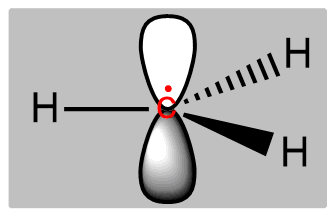
\includegraphics[width=8cm]{ch3.png}
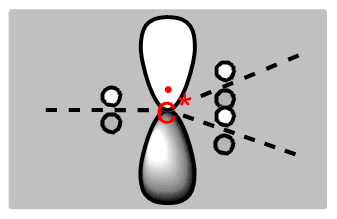
\includegraphics[width=8cm]{pseudoch3.png}
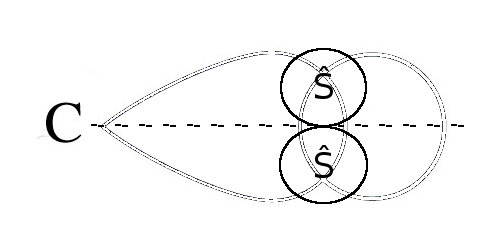
\includegraphics[width=8cm]{tm_sp2_potentials.png}
%\caption{Diagrams of CH\(^{\bullet}_{3}\) (left) and pseudo-CH\(^{\bullet}_{3}\) (right, below) molecules. The pseudo-CH\(^{\bullet}_{3}\) diagrams display the \(s\) and \(p\)-potential positions, and the distances \(d\) and \(c\).}
%\label{figure:ref_pseudo_diagram}
\end{center}
\vspace{0.25in}
\hspace*{3in}
\caption{Diagrams of CH\(^{\bullet}_{3}\) (left) and pseudo-CH\(^{\bullet}_{3}\) (right, below) molecules. The pseudo-CH\(^{\bullet}_{3}\) diagrams display the \(s\) and \(p\)-potential positions, and the distances \(d\) and \(c\).}
\label{figure:ref_pseudo_diagram}
\end{figure}

\begin{figure}
%\vspace*{0.1in}   %%% FIGURE 2
\begin{center}
%\includegraphics[width=0.2\columnwidth,keepaspectratio=true]{cc.eps}
\fbox{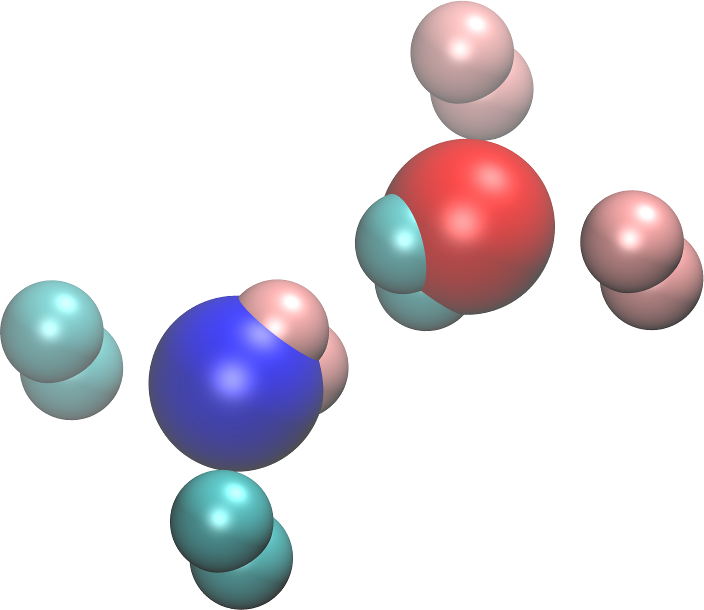
\includegraphics[width=0.45\textwidth]{hires_long_r_crop.png}}%
\fbox{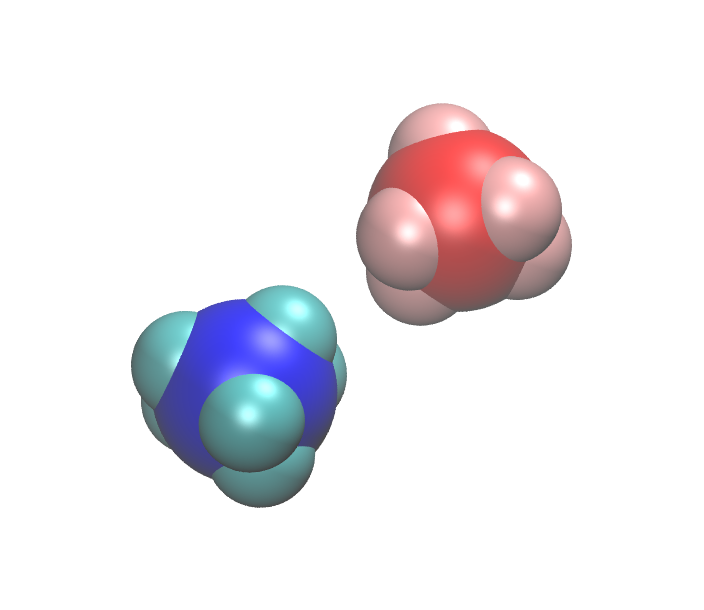
\includegraphics[width=0.45\textwidth]{hires_short_r_crop.png}}
%\caption{Diagrams of pseudo-ethene with \(d =\) 2.0 a.u. (left), and \(d = 0.5\) a.u. (right). The first pseudo-carbon is displayed in blue, with its \(s\) pseudo-potentials in cyan, and the second pseudo-carbon is in red, with its potentials in pink.}
%\label{fig:long_r_ethene}
\end{center}
\vspace{0.25in}
\hspace*{3in}

\caption{Diagrams of pseudo-ethene with \(d =\) 2.0 a.u. (left), and \(d = 0.5\) a.u. (right). The first pseudo-carbon is displayed in blue, with its \(s\) pseudo-potentials in cyan, and the second pseudo-carbon is in red, with its potentials in pink.}
\label{fig:long_r_ethene}
\end{figure}

\begin{figure}
%\vspace*{0.1in}   %%% FIGURE 3
\begin{center}
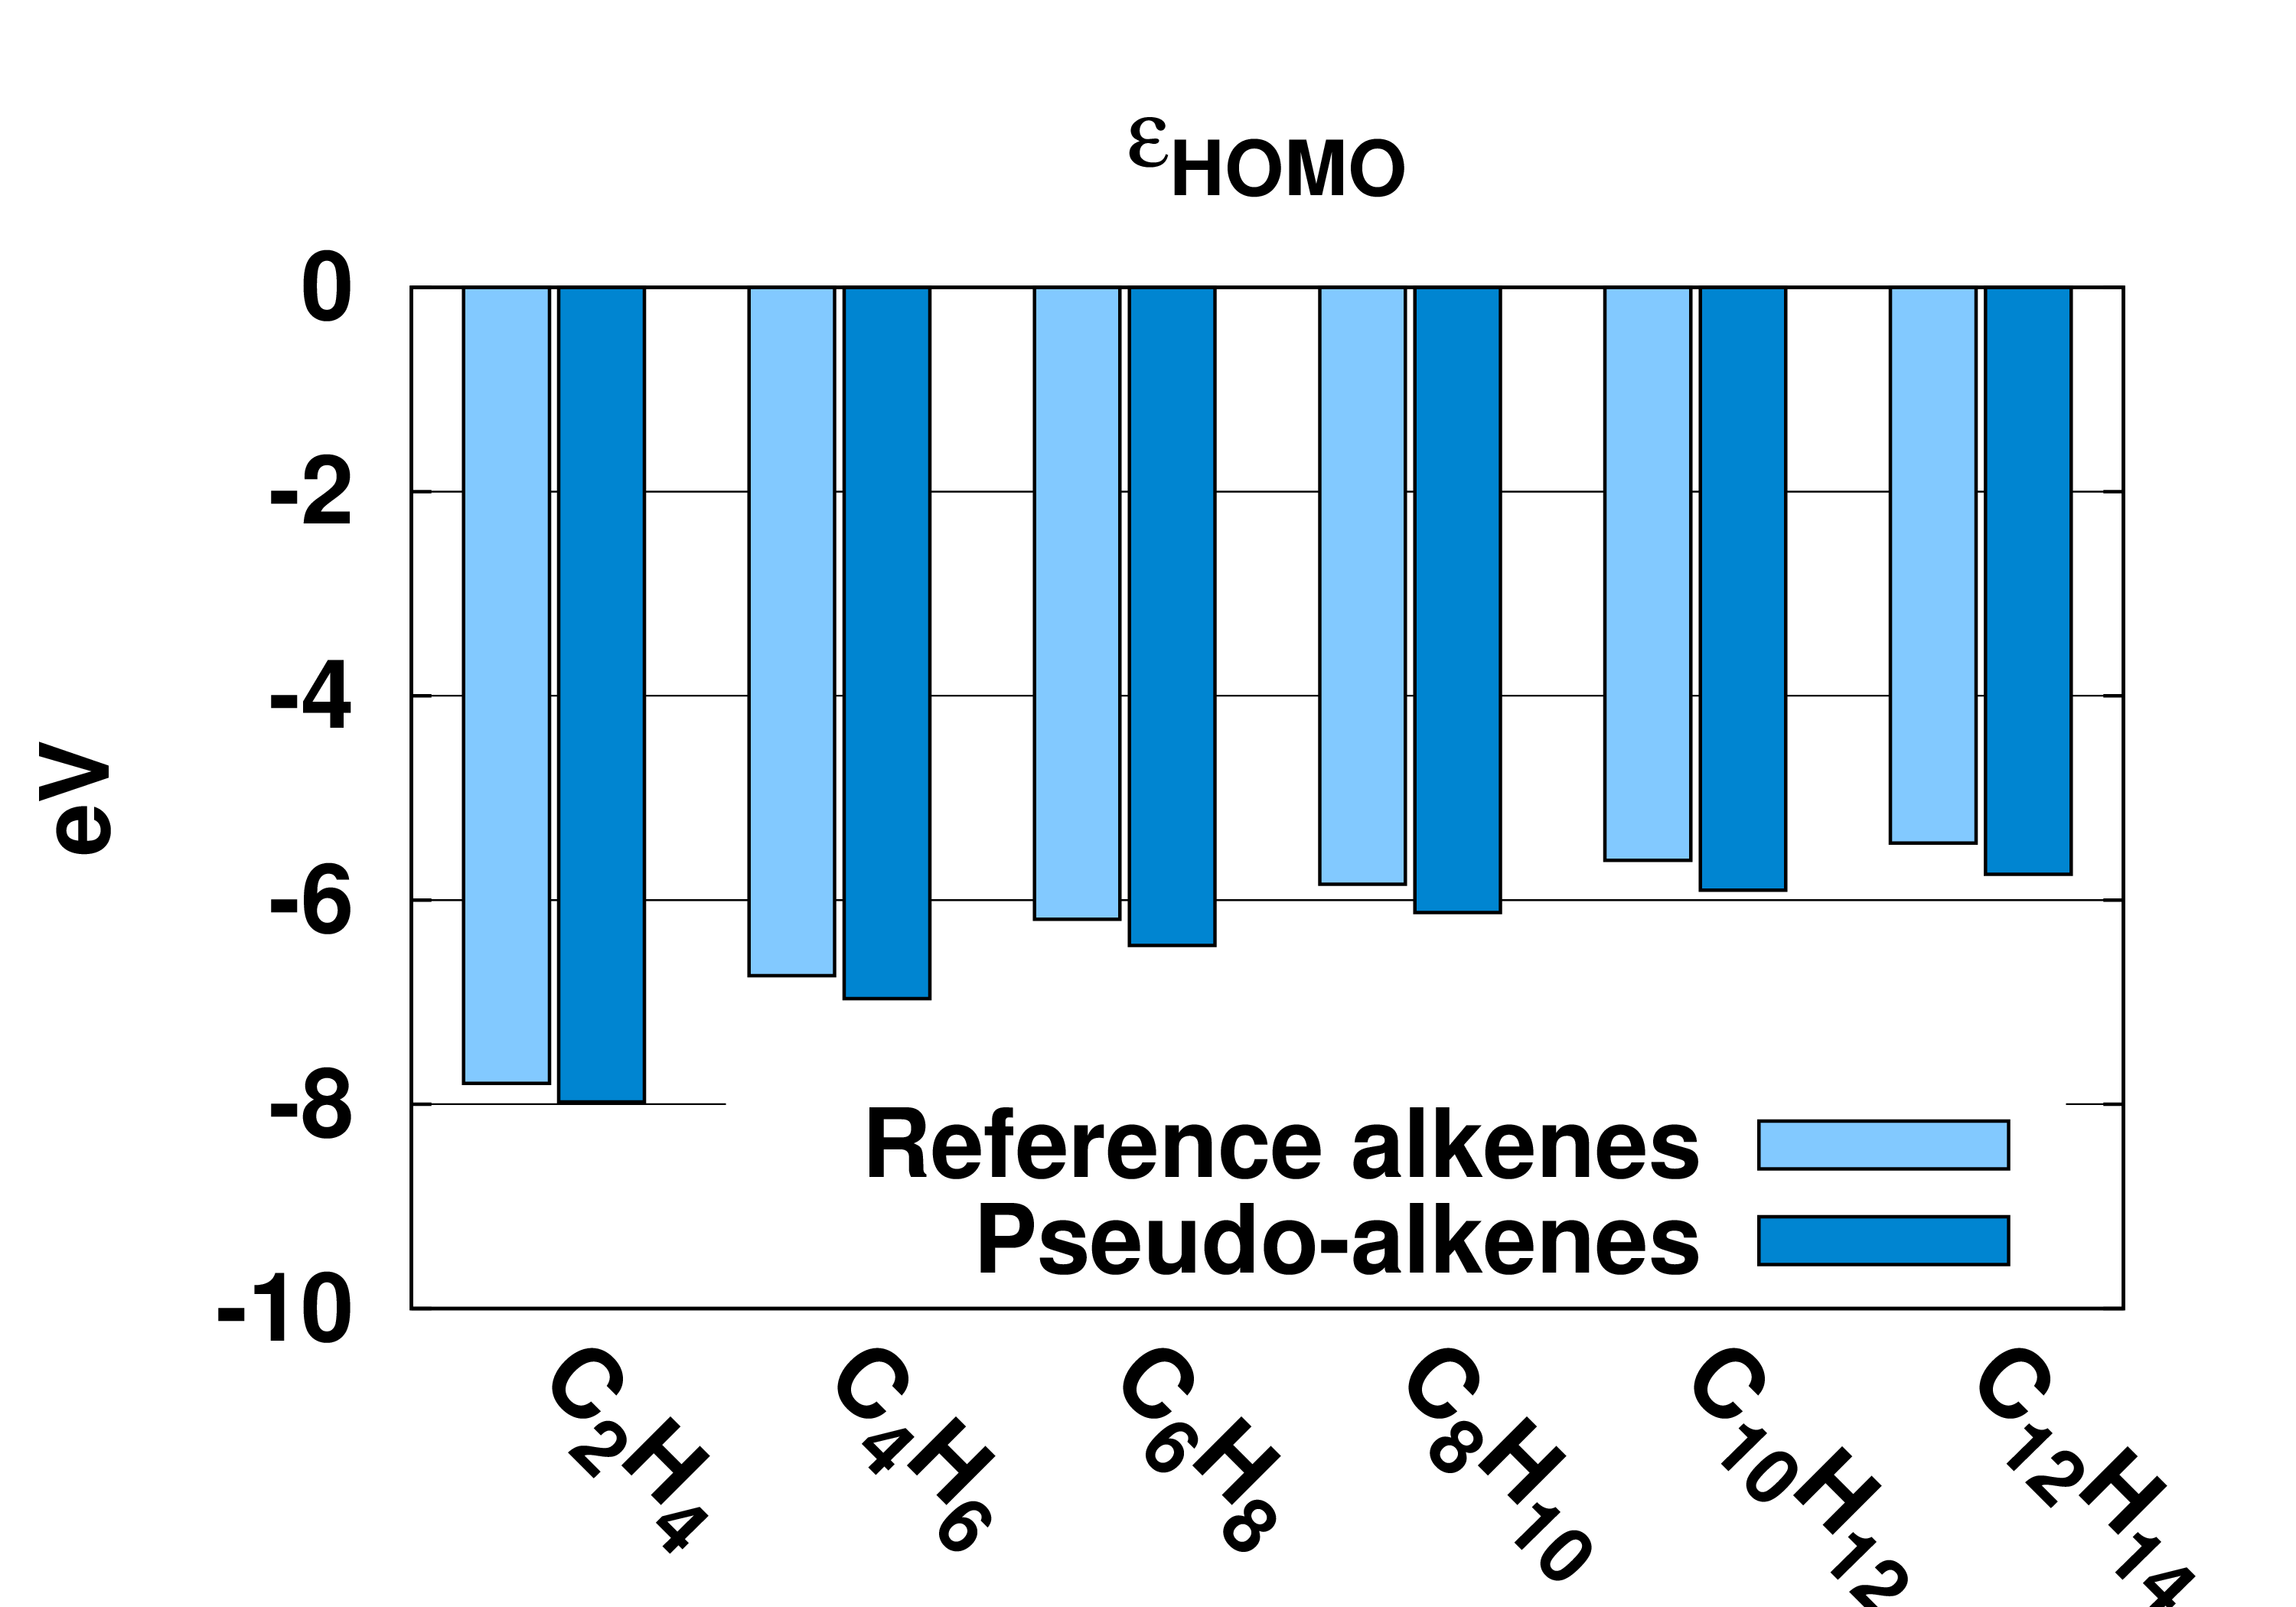
\includegraphics[width=8cm]{short_pbe0_homo}
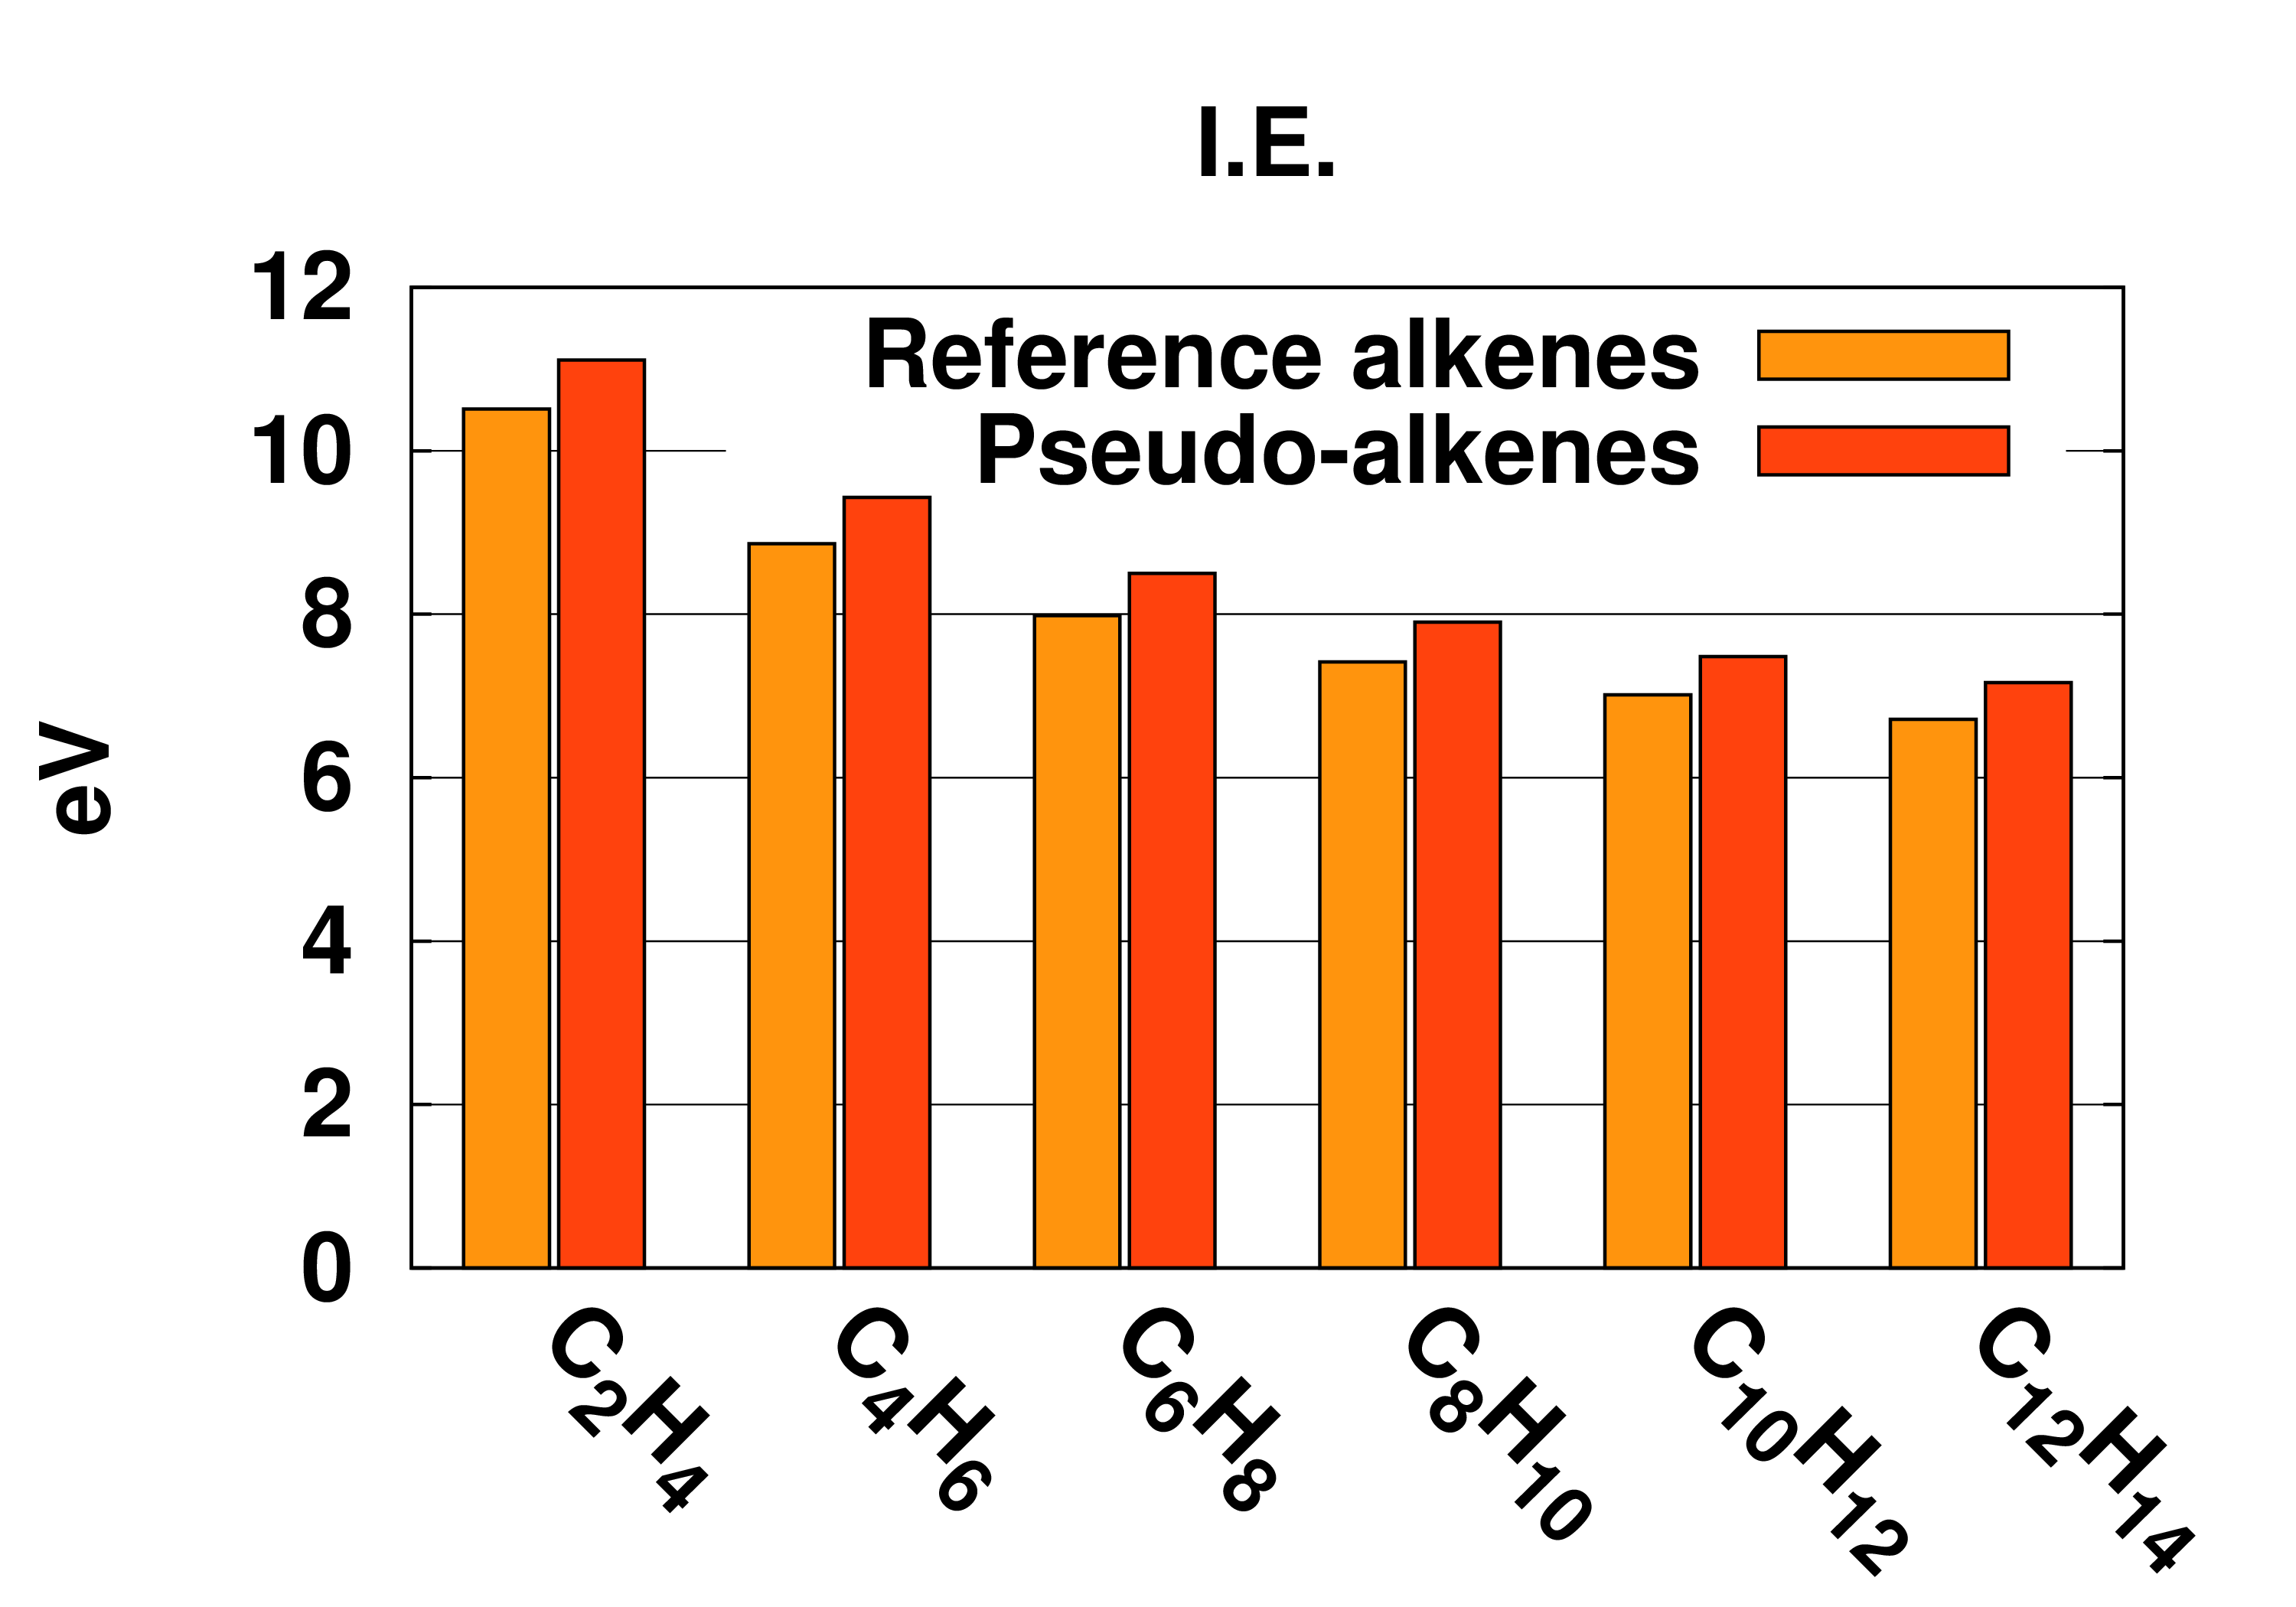
\includegraphics[width=8cm]{short_pbe0_ie}
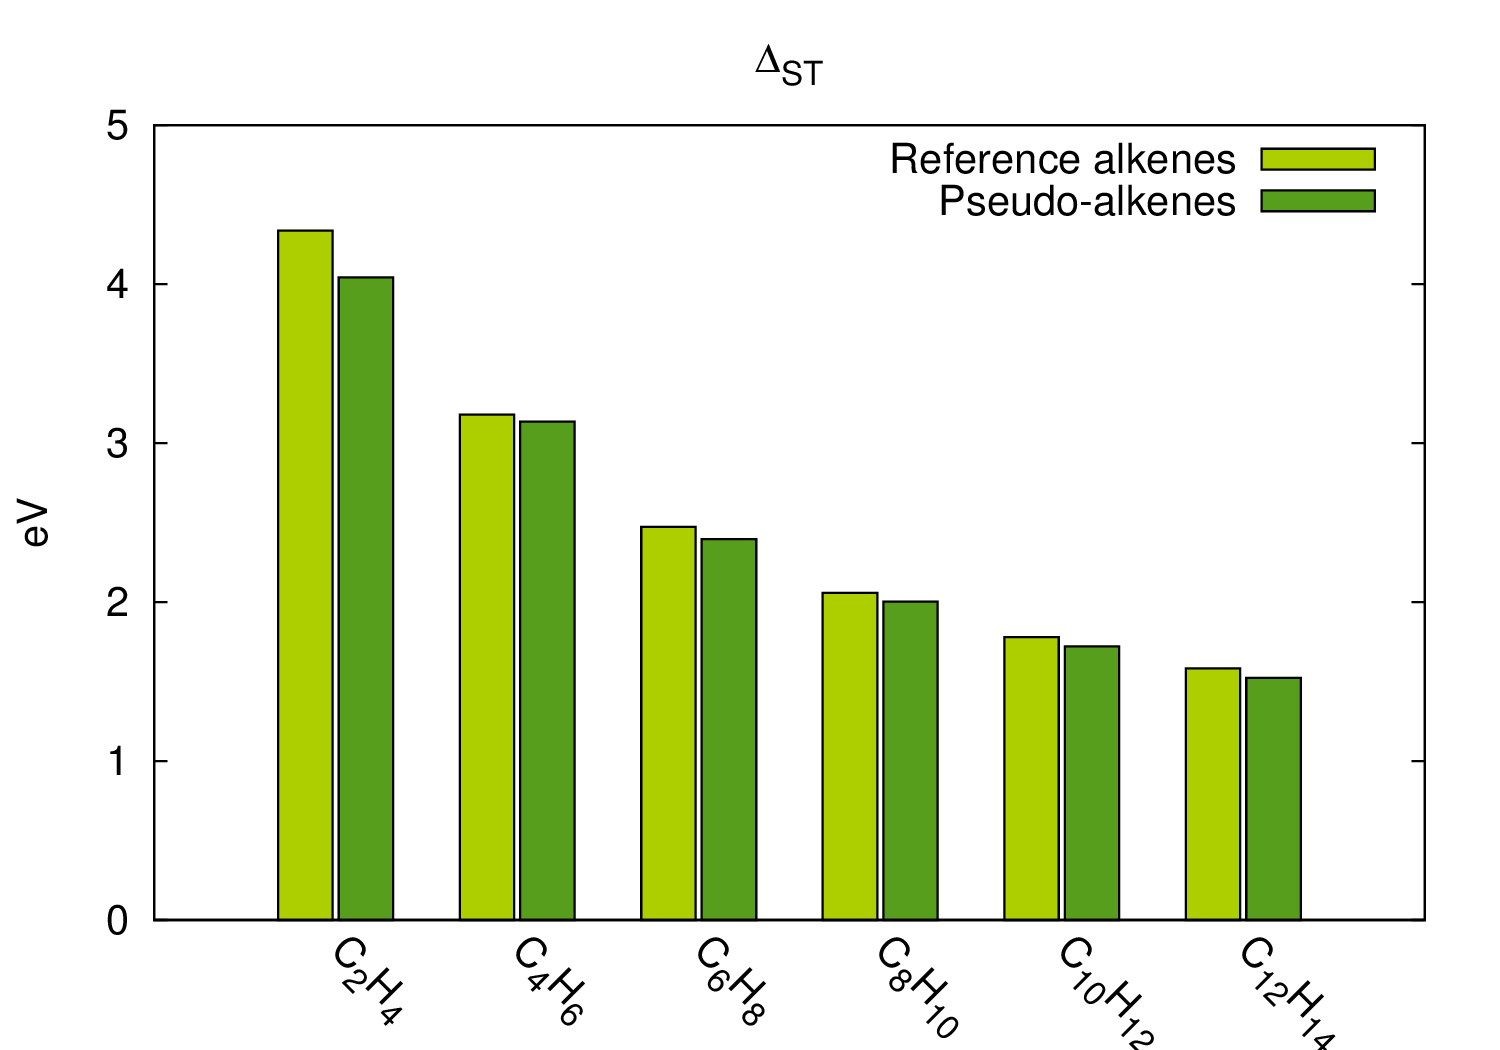
\includegraphics[width=8cm]{short_pbe0_st}
%\caption{DFT (PBE0) comparison of reference and pseudo-system energies across a range of chain alkenes.}
%\label{fig:alkenes_hf_dft}
\end{center}
\vspace{0.25in}
\hspace*{3in}

\caption{DFT (PBE0) comparison of reference and pseudo-system energies across a range of chain alkenes.}
\label{fig:alkenes_hf_dft}
\end{figure}

\begin{figure}
%\vspace*{0.1in}   %%% FIGURE 4
\begin{center}
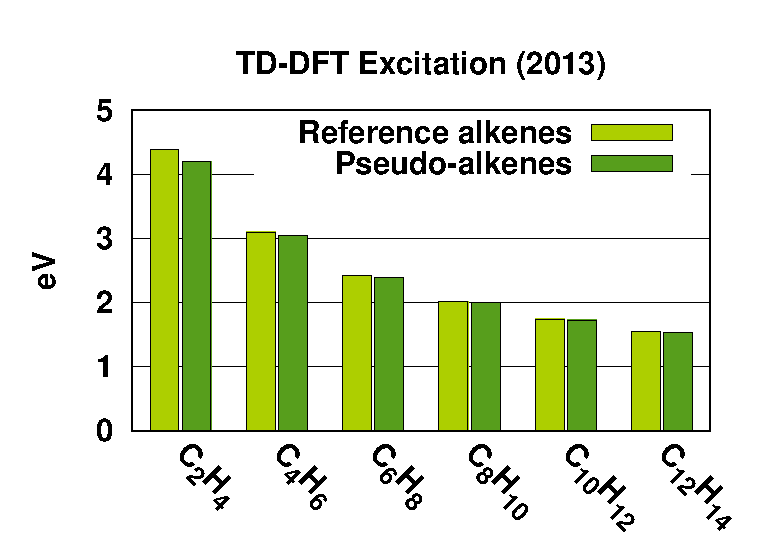
\includegraphics[width=8cm]{short_pbe0_tddft_2013}
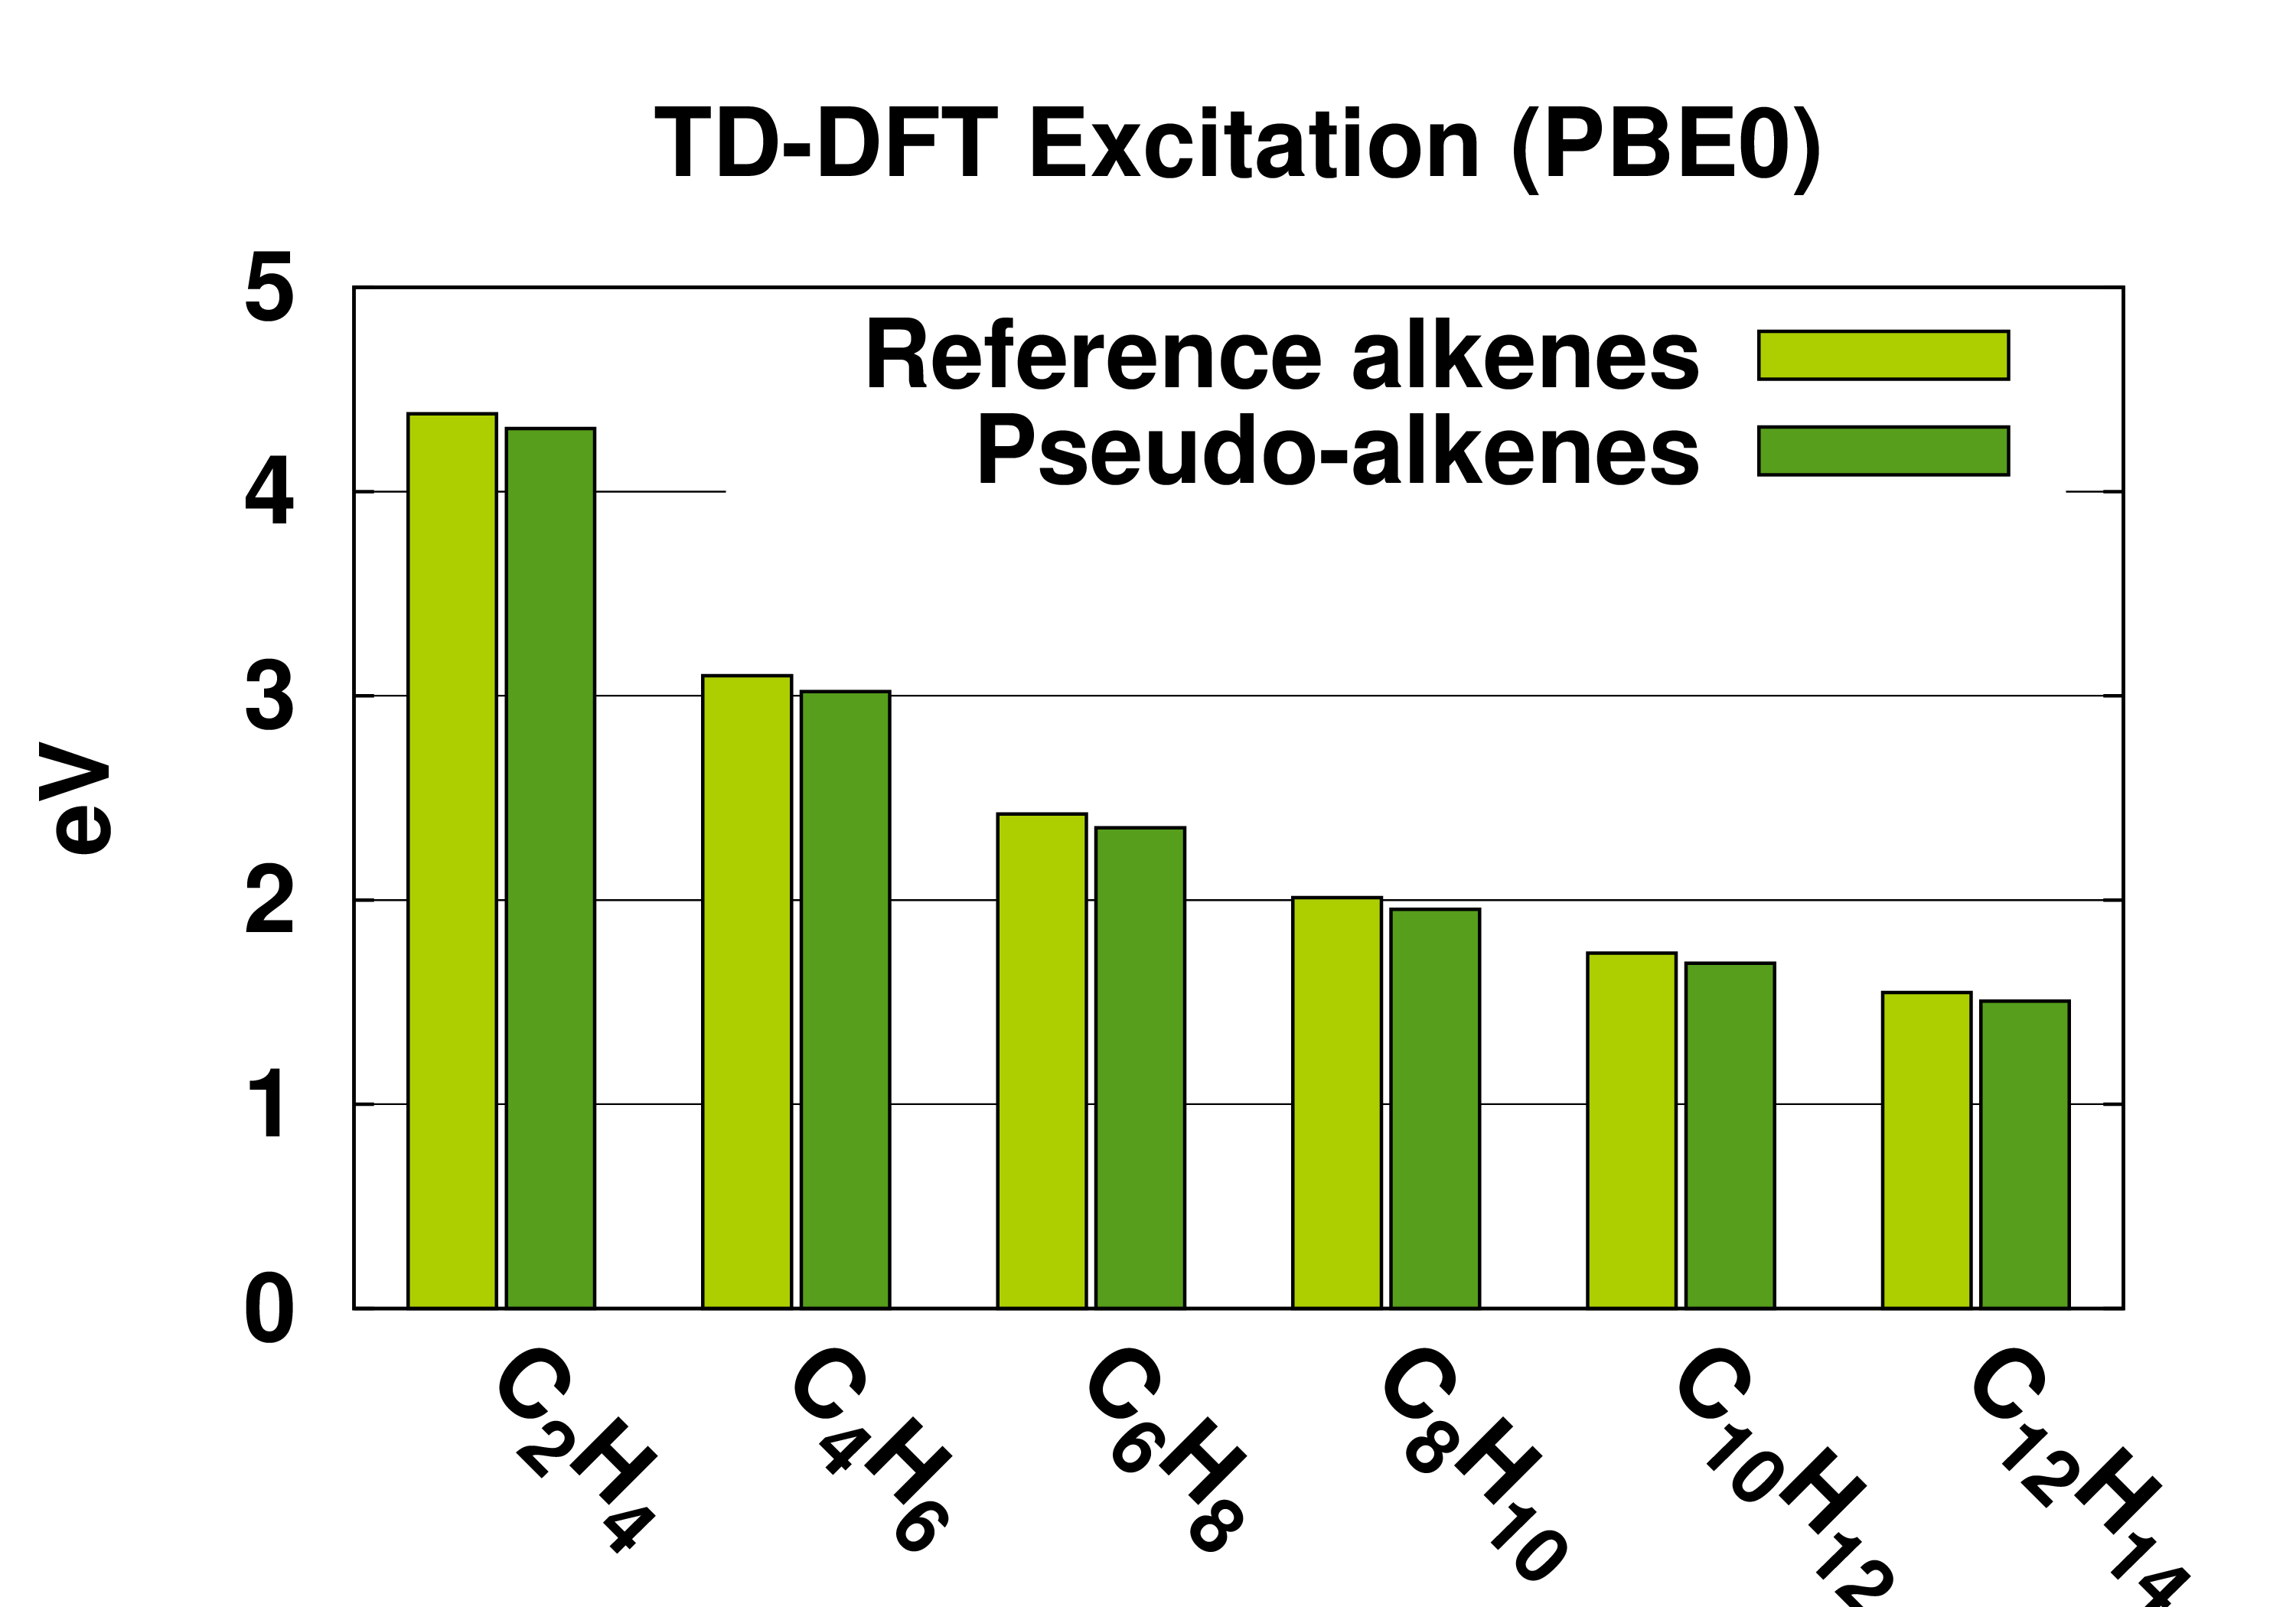
\includegraphics[width=8cm]{short_pbe0_tddft}
%\caption{Comparison of pseudo-alkenes with previous\cite{drujon_pseudopotentials_2013} and current potentials using TD-DFT excitation energies.}
%\label{fig:alkenes_tddft}
\end{center}
\vspace{0.25in}
\hspace*{3in}

\caption{Comparison of pseudo-alkenes with previous\cite{drujon_pseudopotentials_2013} and current potentials using TD-DFT excitation energies.}
\label{fig:alkenes_tddft}
\end{figure}

\begin{figure}
%\vspace*{0.1in}   %%% FIGURE 5
\begin{center}
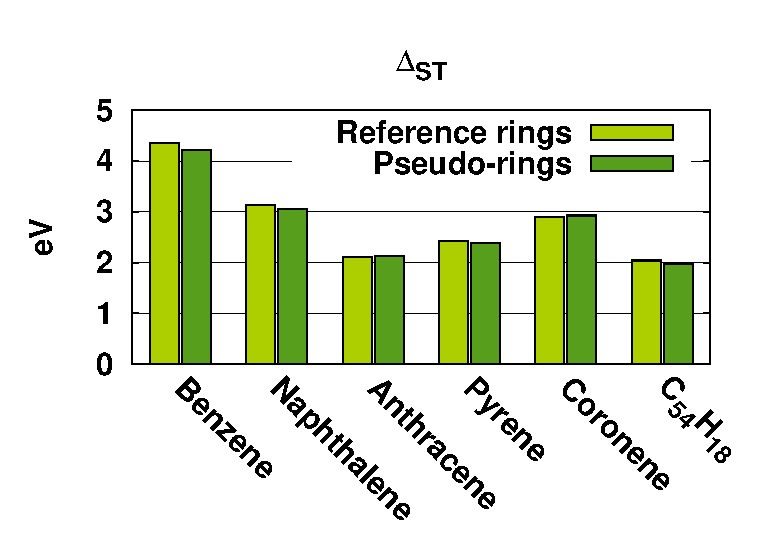
\includegraphics[width=8cm]{ring_pbe0_st}
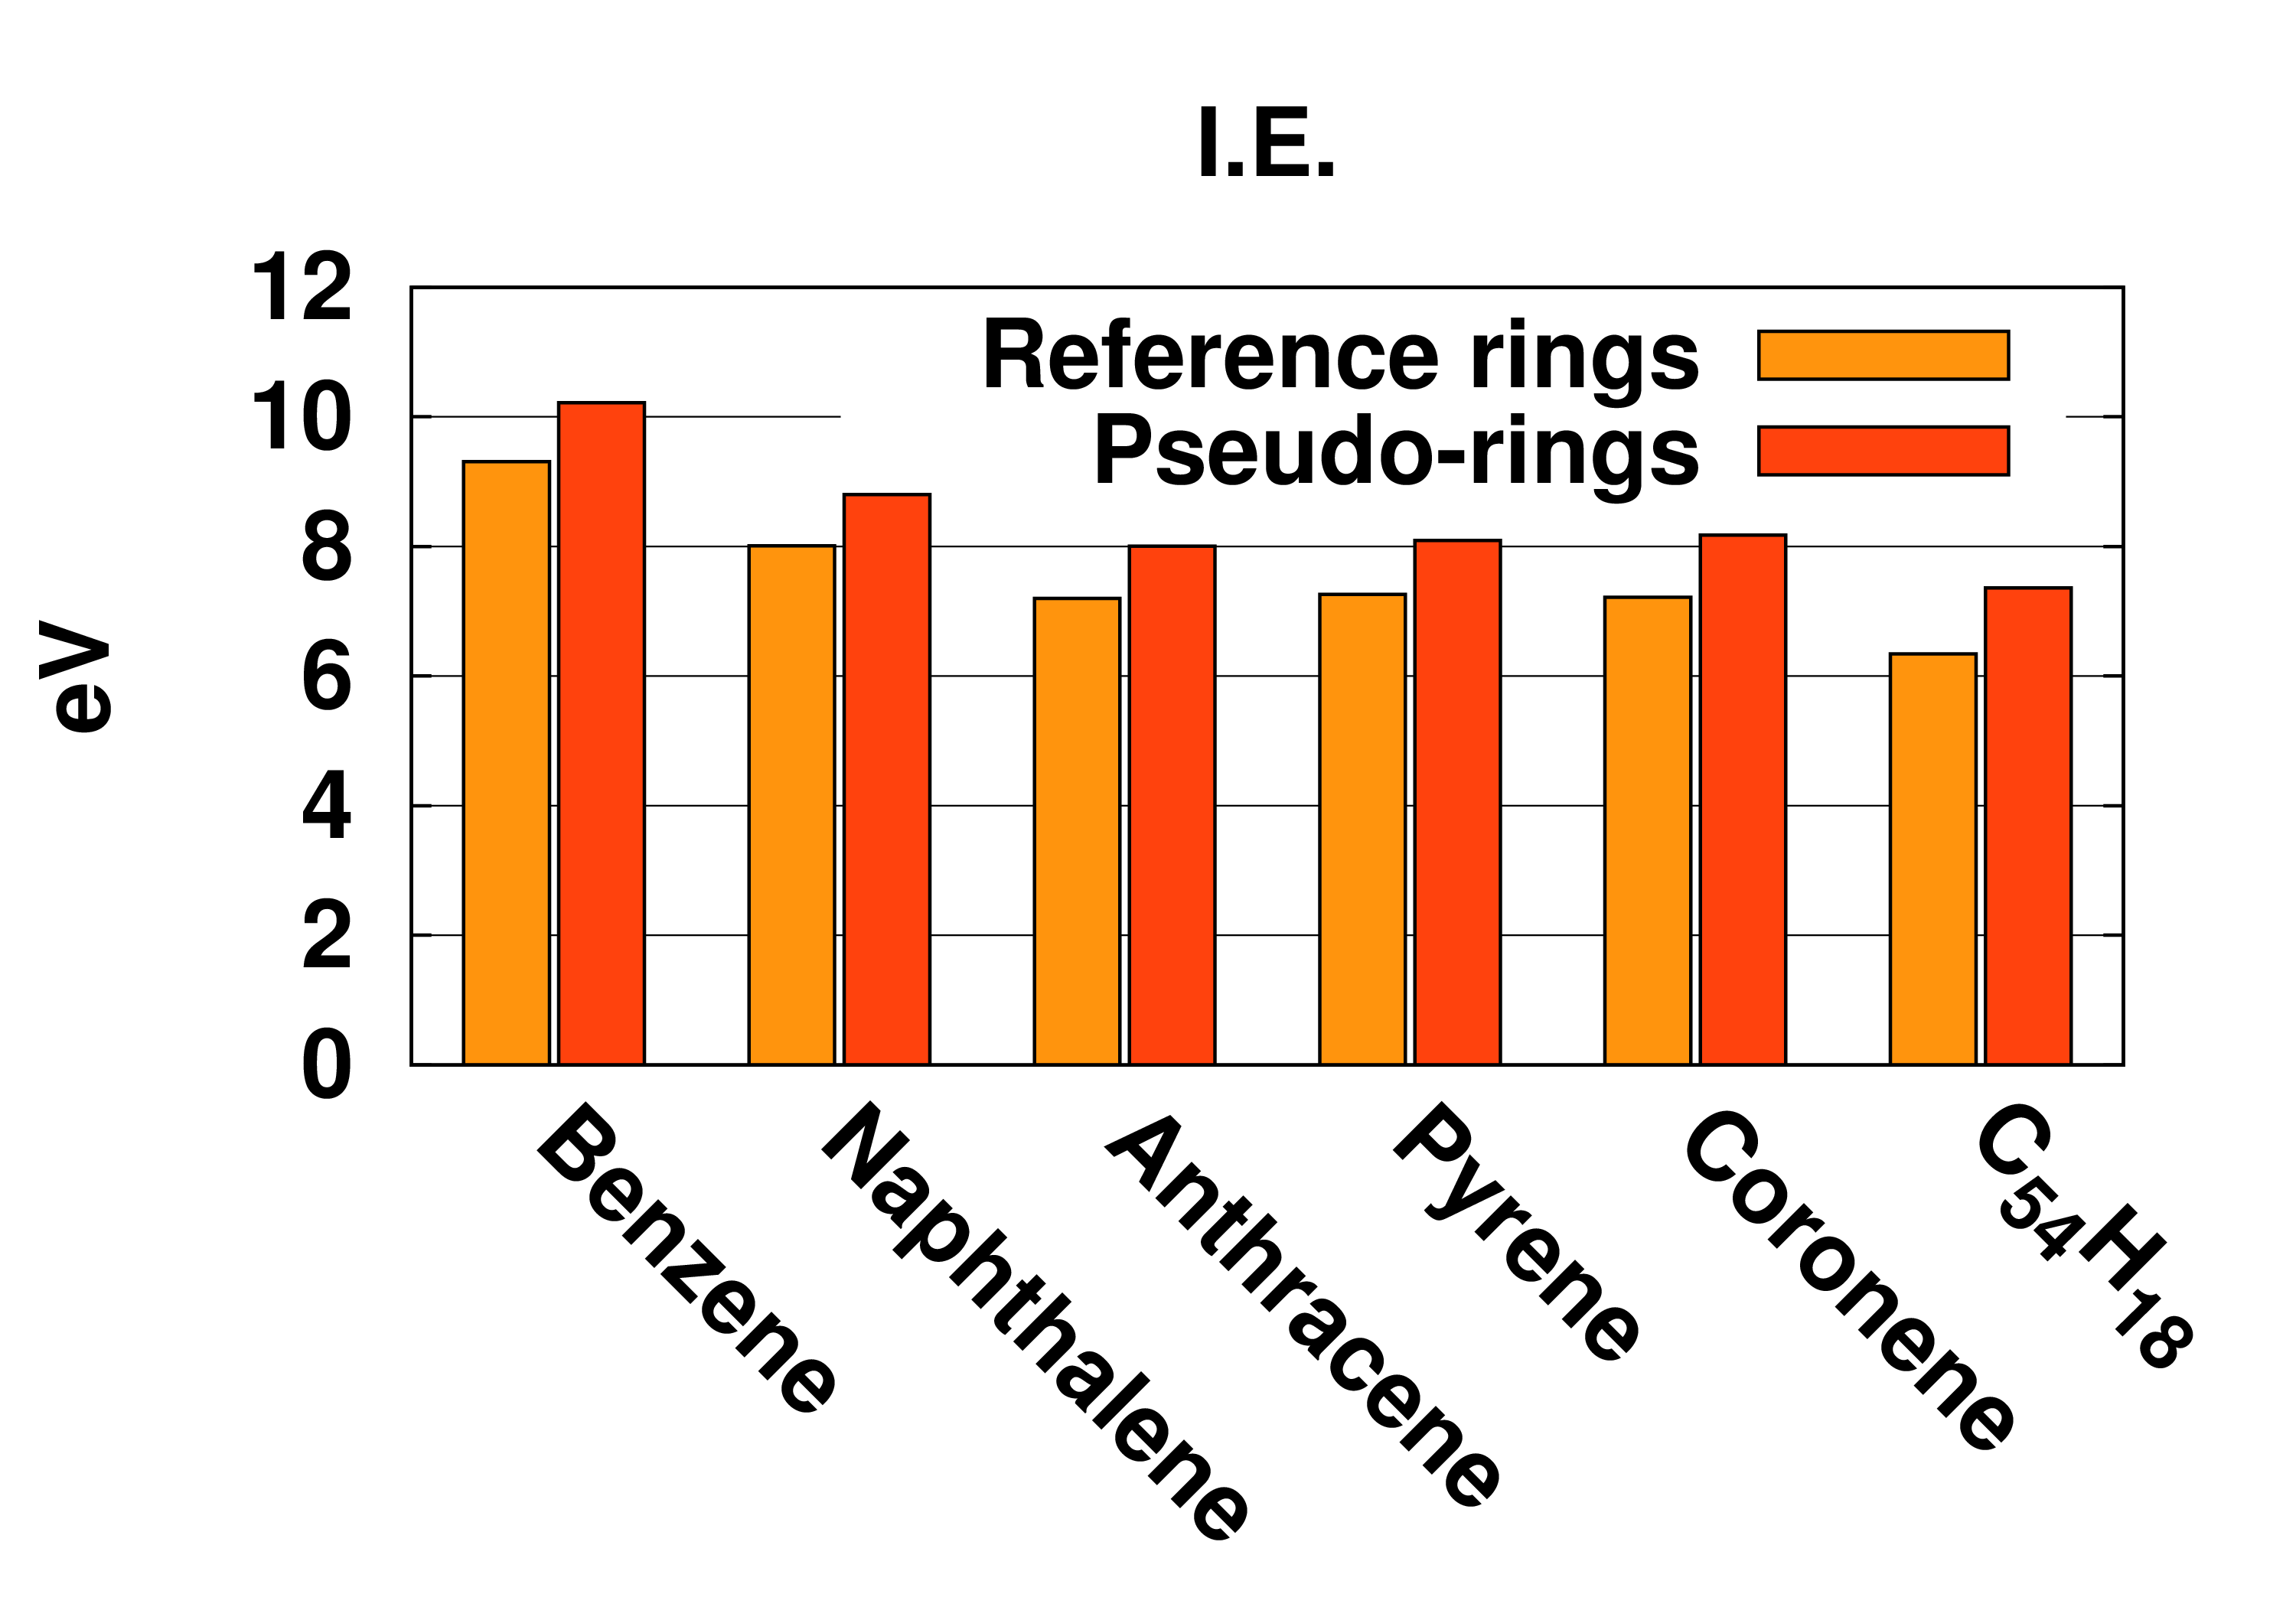
\includegraphics[width=8cm]{ring_pbe0_ie}
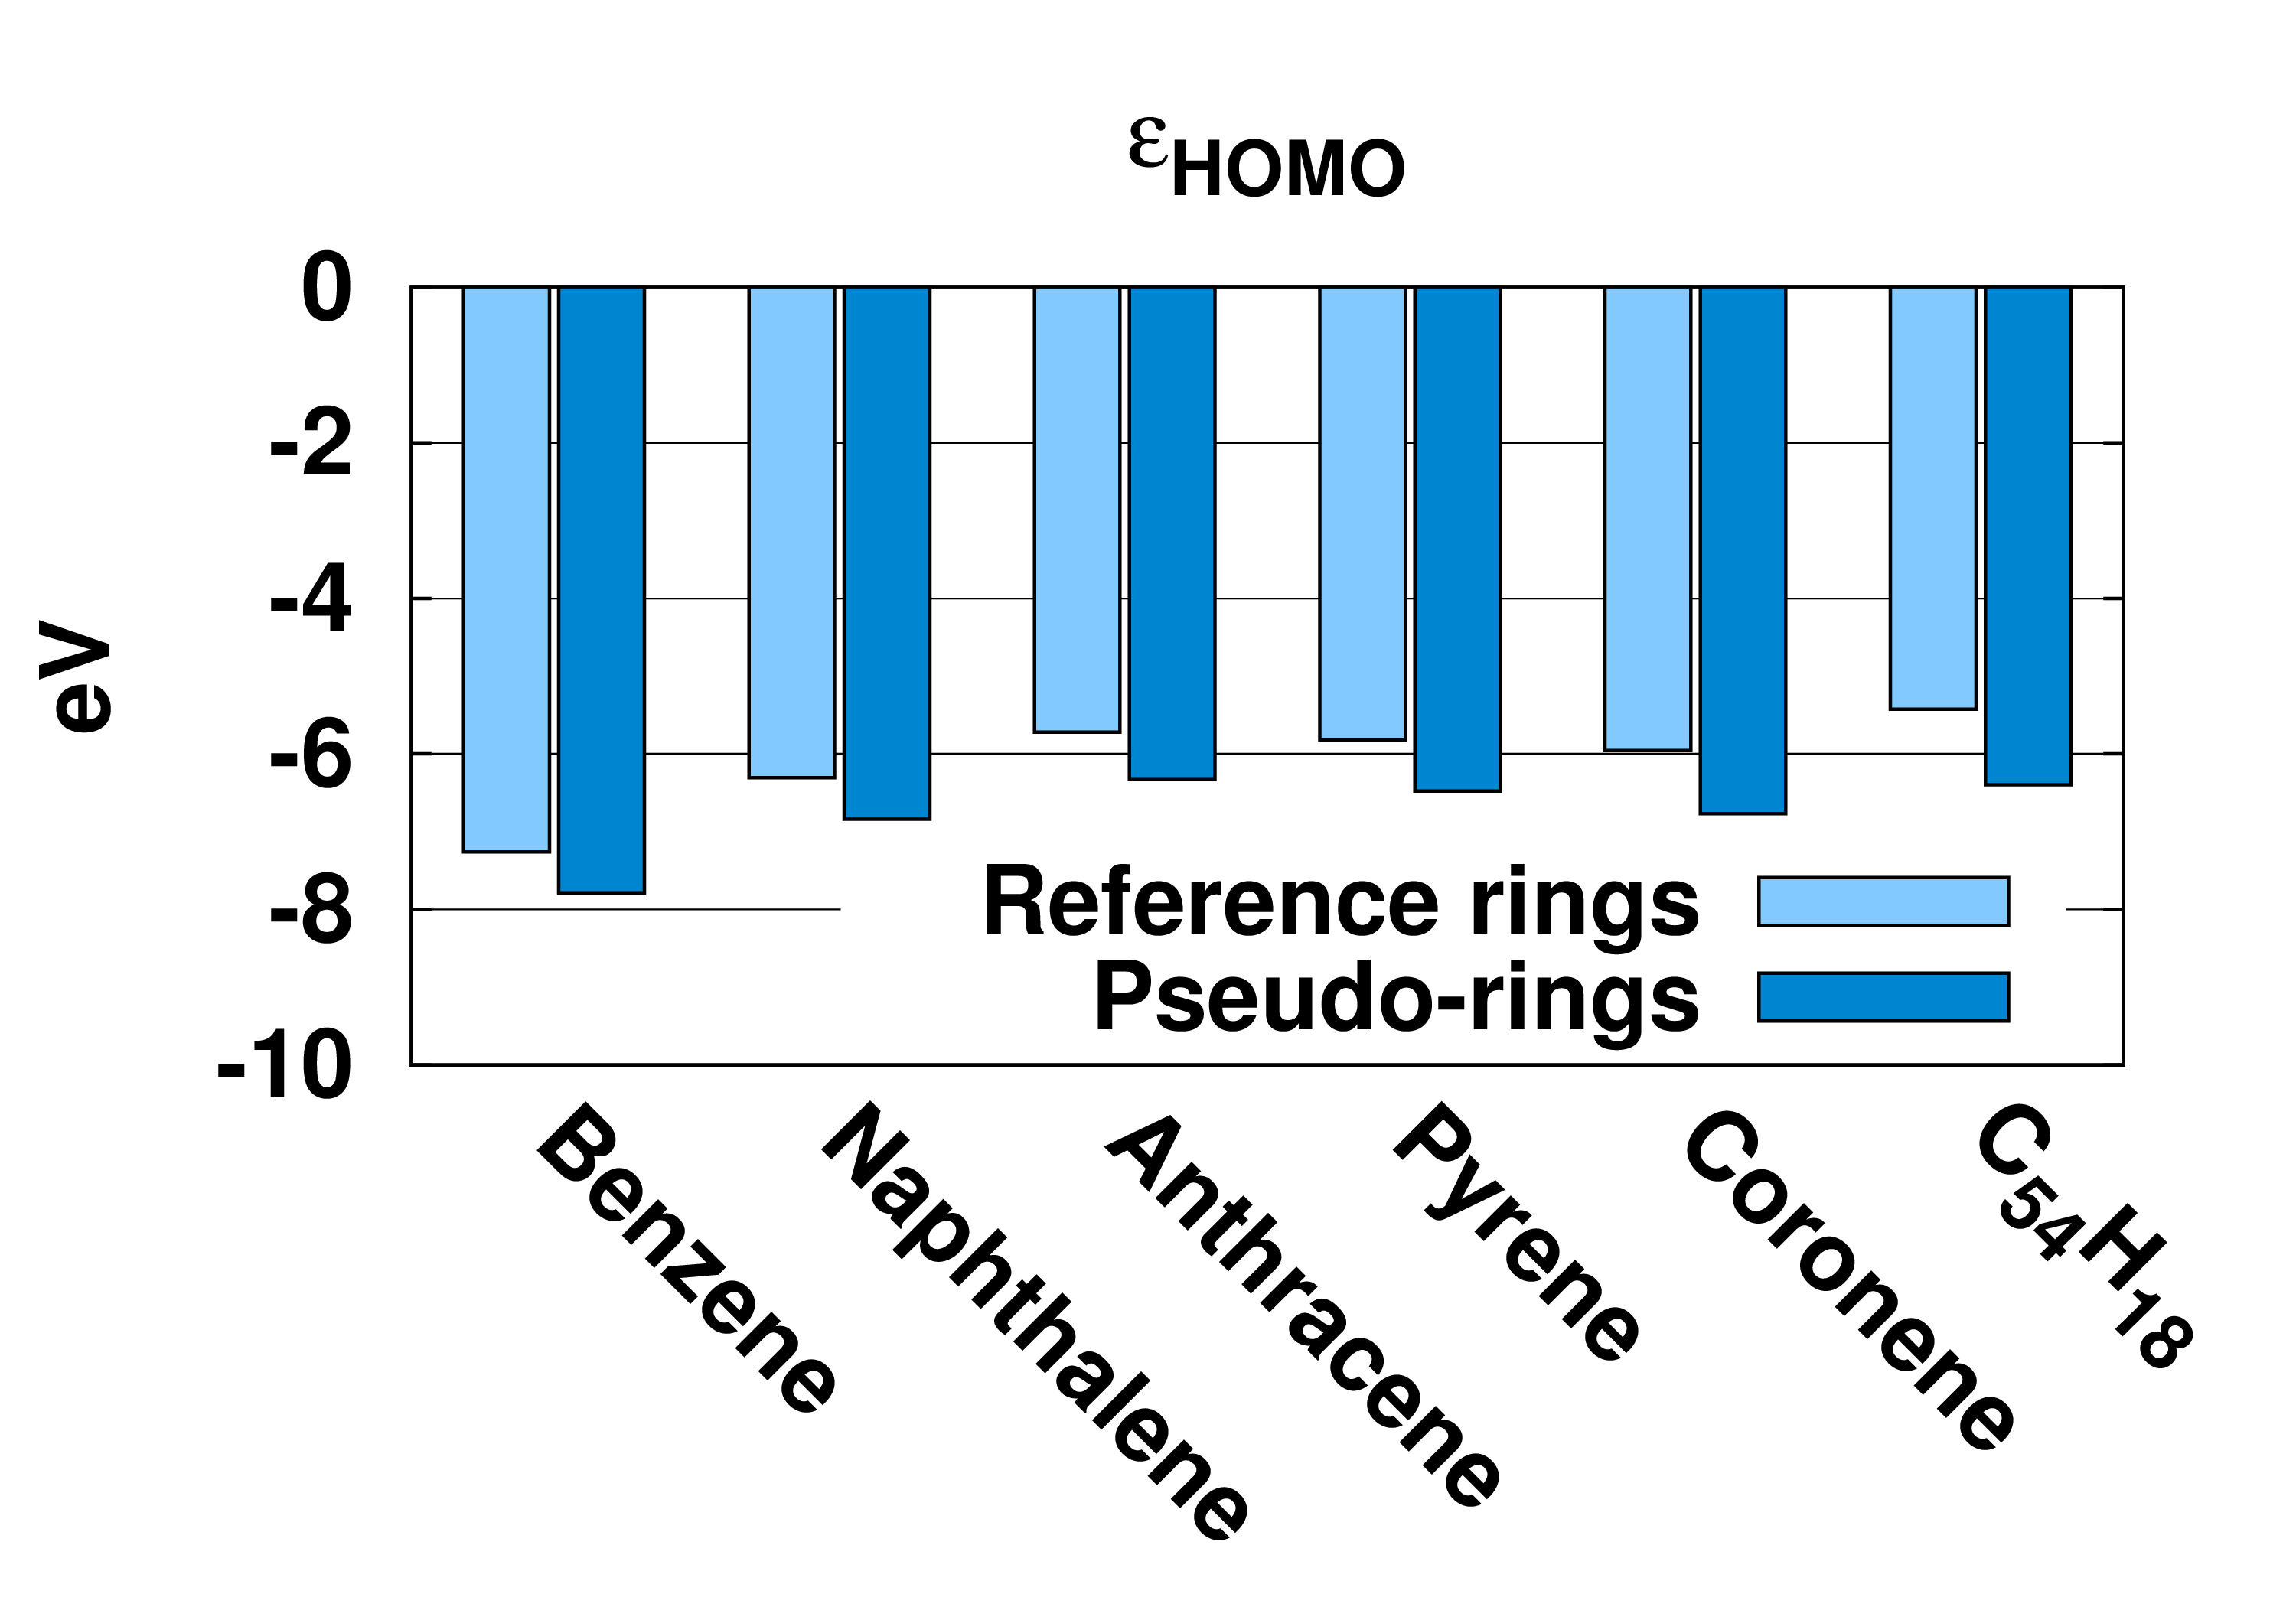
\includegraphics[width=8cm]{ring_pbe0_homo}
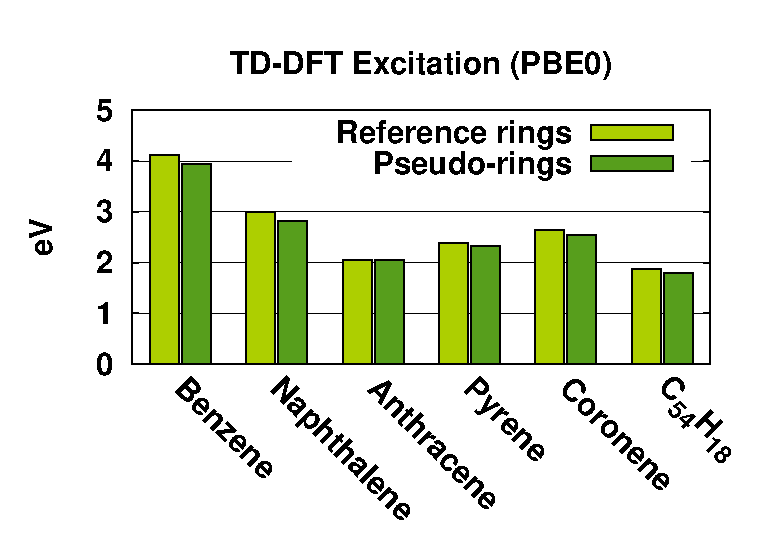
\includegraphics[width=8cm]{ring_pbe0_tddft}
%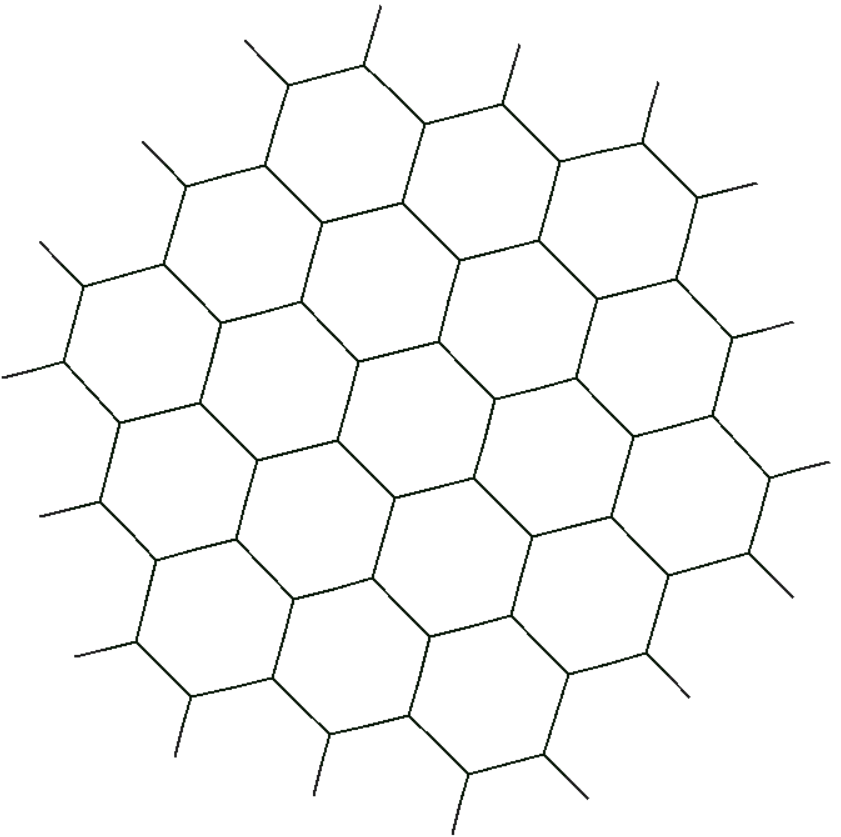
\includegraphics[width=5cm]{19_ring_diagram}
\fbox{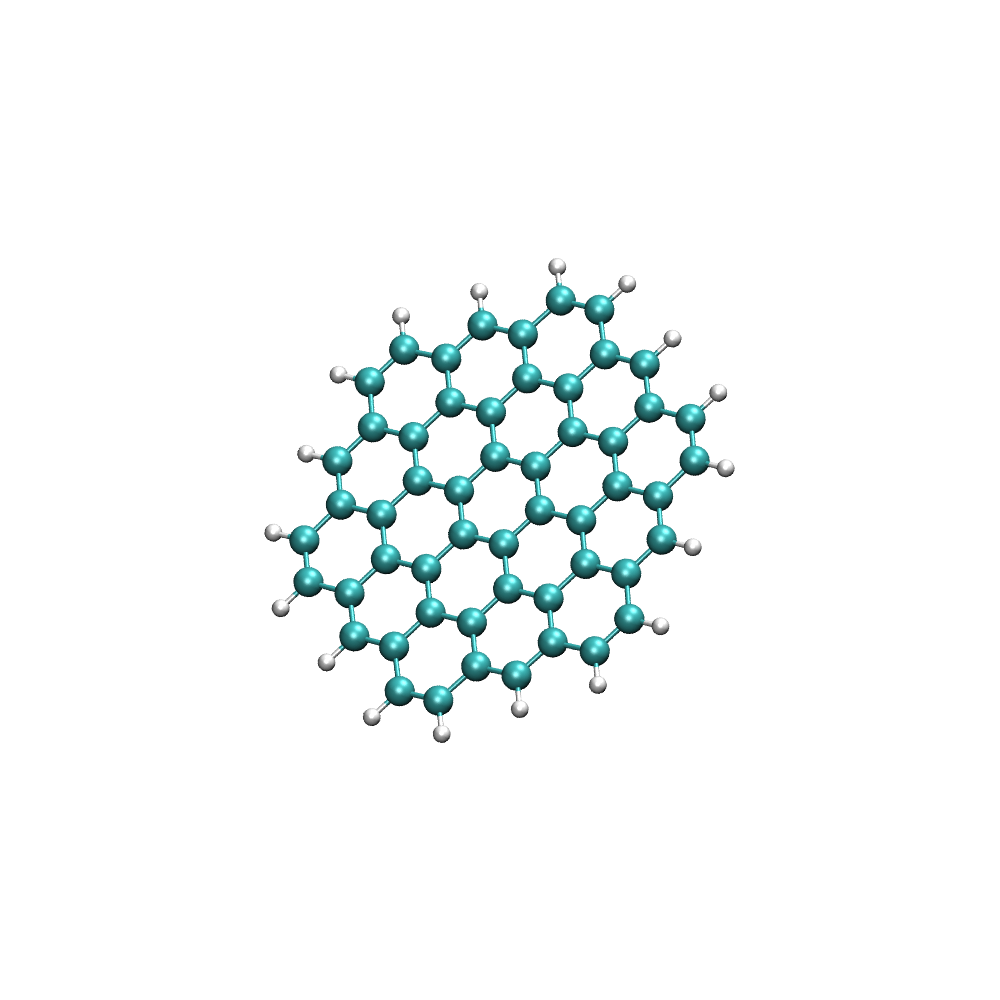
\includegraphics[width=5cm]{c54h18}}
%\caption{DFT and TD-DFT (PBE0) comparison of reference and pseudo-system energies across a range of ring molecules. 
%C\(_{54}\)H\(_{18}\) is shown in the bottom.}
%\label{fig:rings_graphs}
\end{center}
\vspace{0.25in}
\hspace*{3in}

\caption{DFT and TD-DFT (PBE0) comparison of reference and pseudo-system energies across a range of ring molecules. 
C\(_{54}\)H\(_{18}\) is shown in the bottom.}
\label{fig:rings_graphs}
\end{figure}

\begin{figure}
%\vspace*{0.1in}   %%% FIGURE 6
\begin{center}
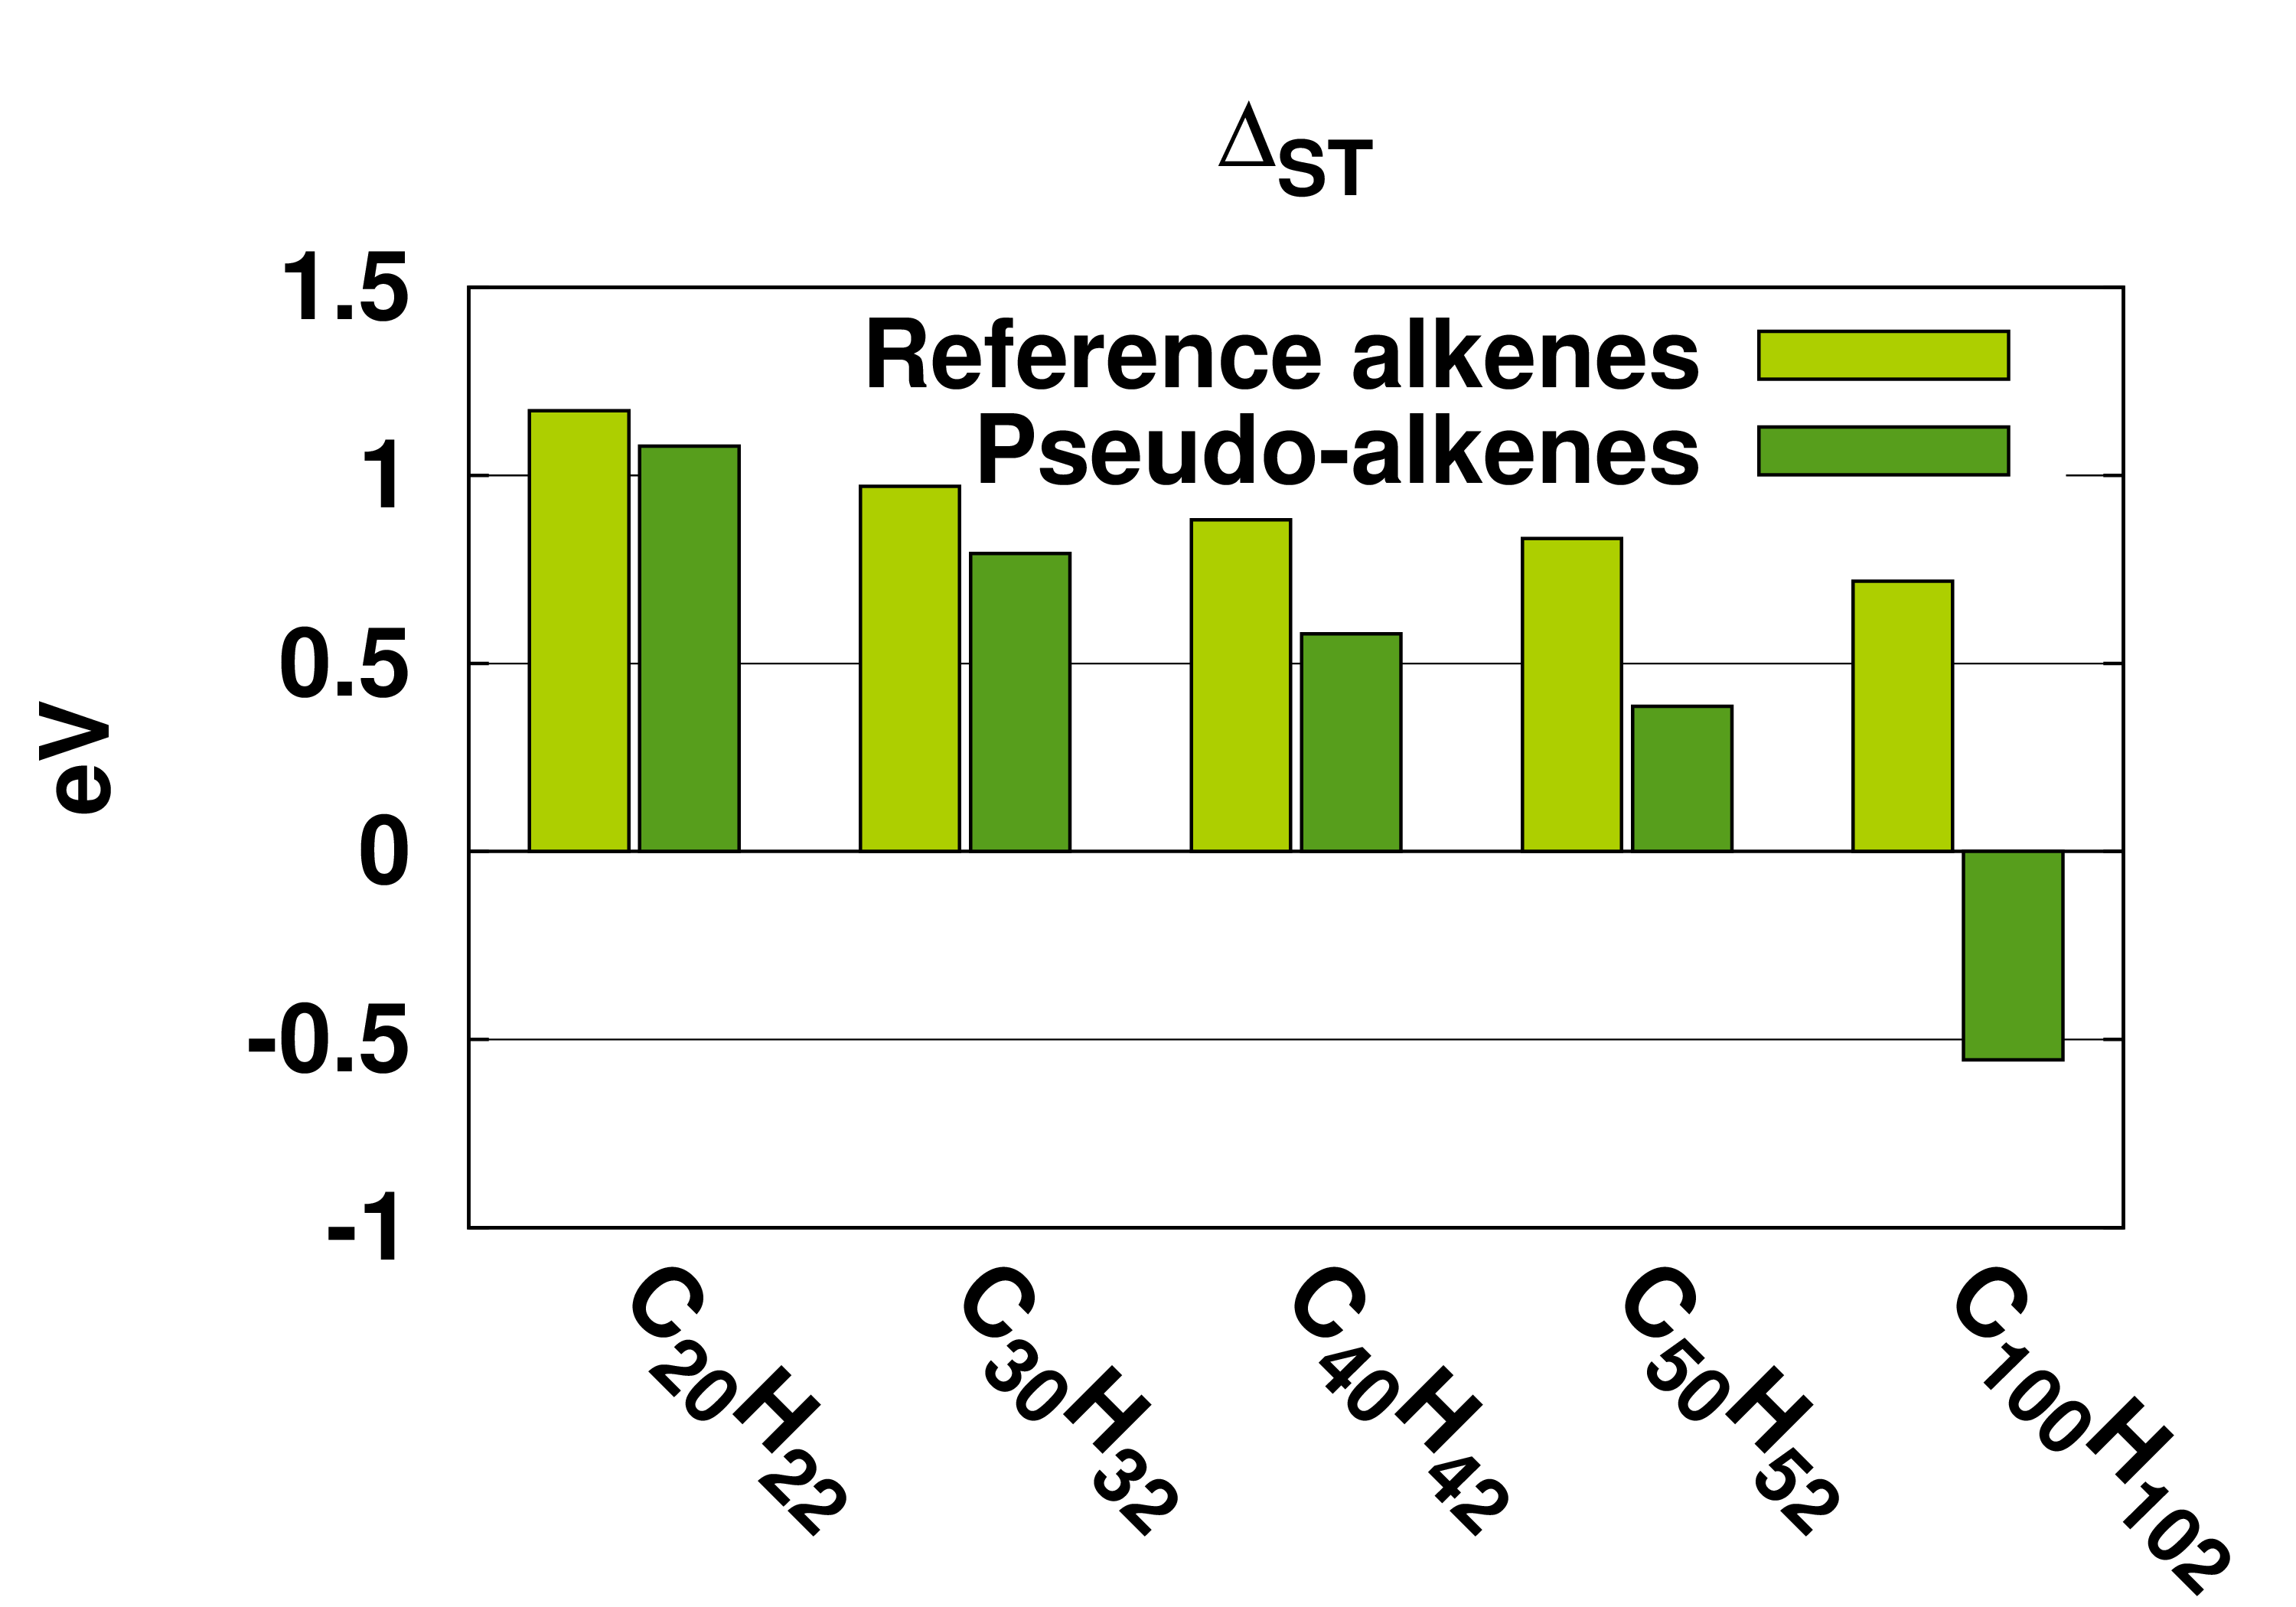
\includegraphics[width=8cm]{long_pbe0_st}
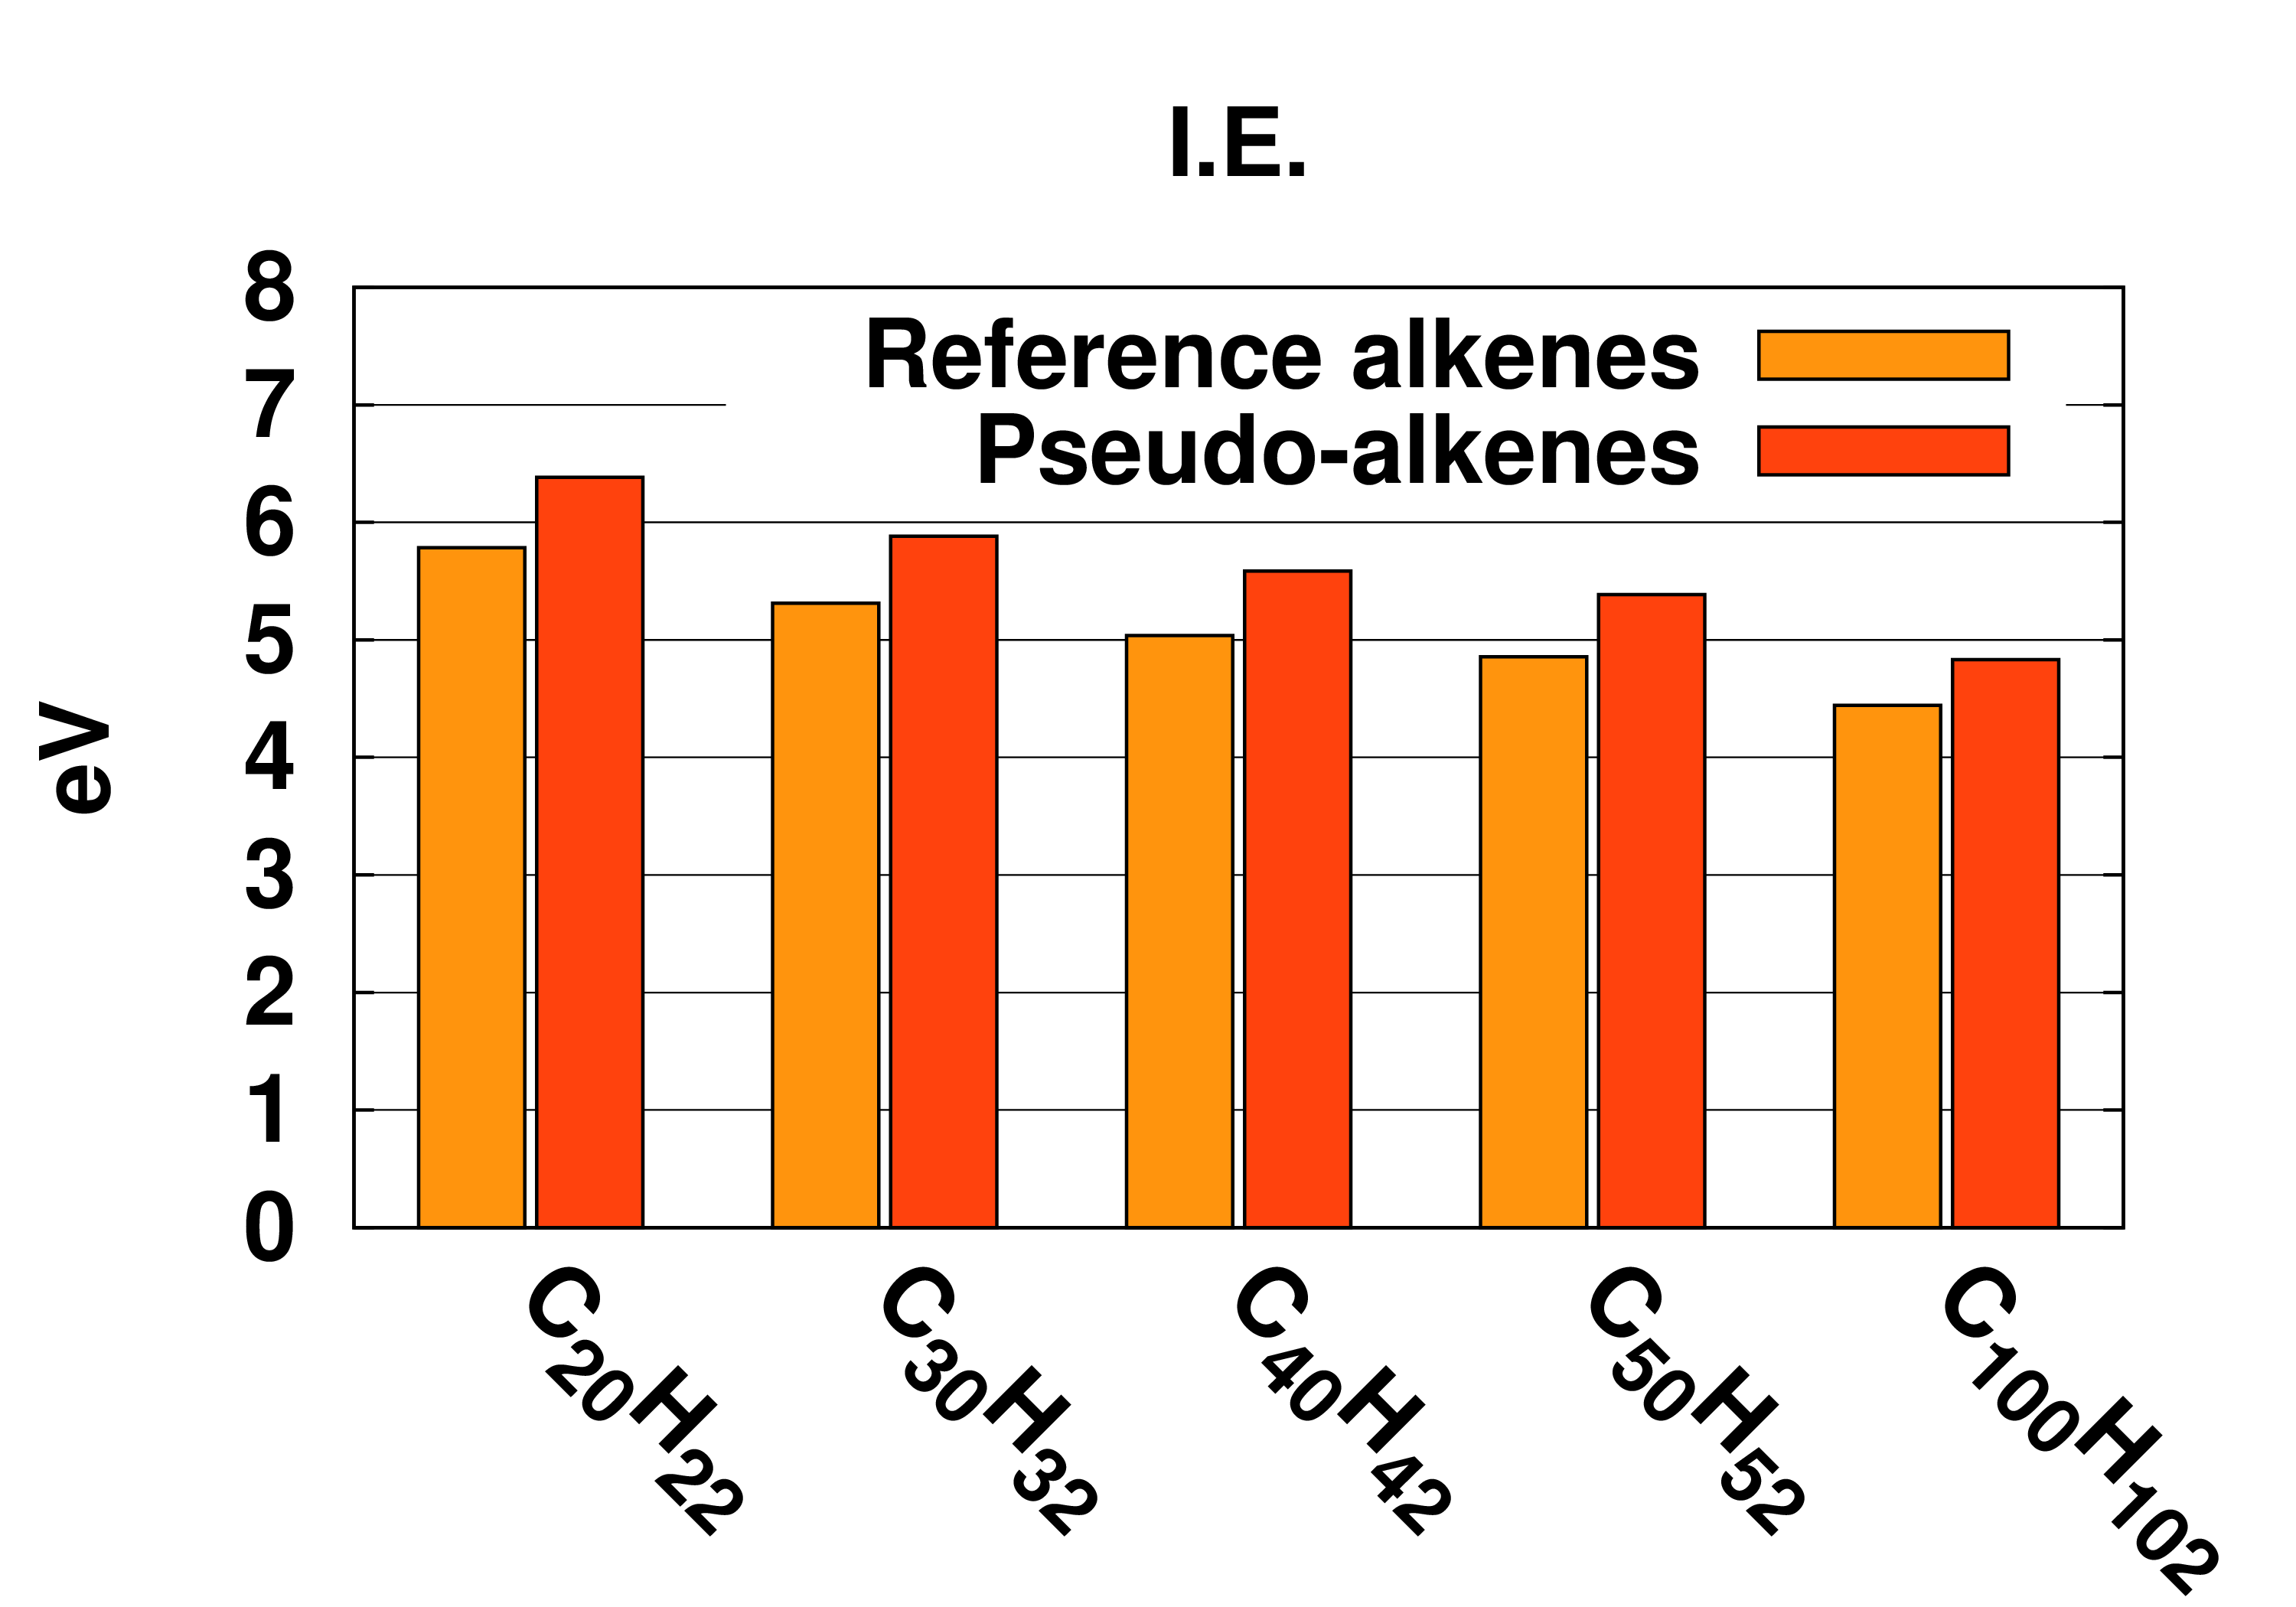
\includegraphics[width=8cm]{long_pbe0_ie}
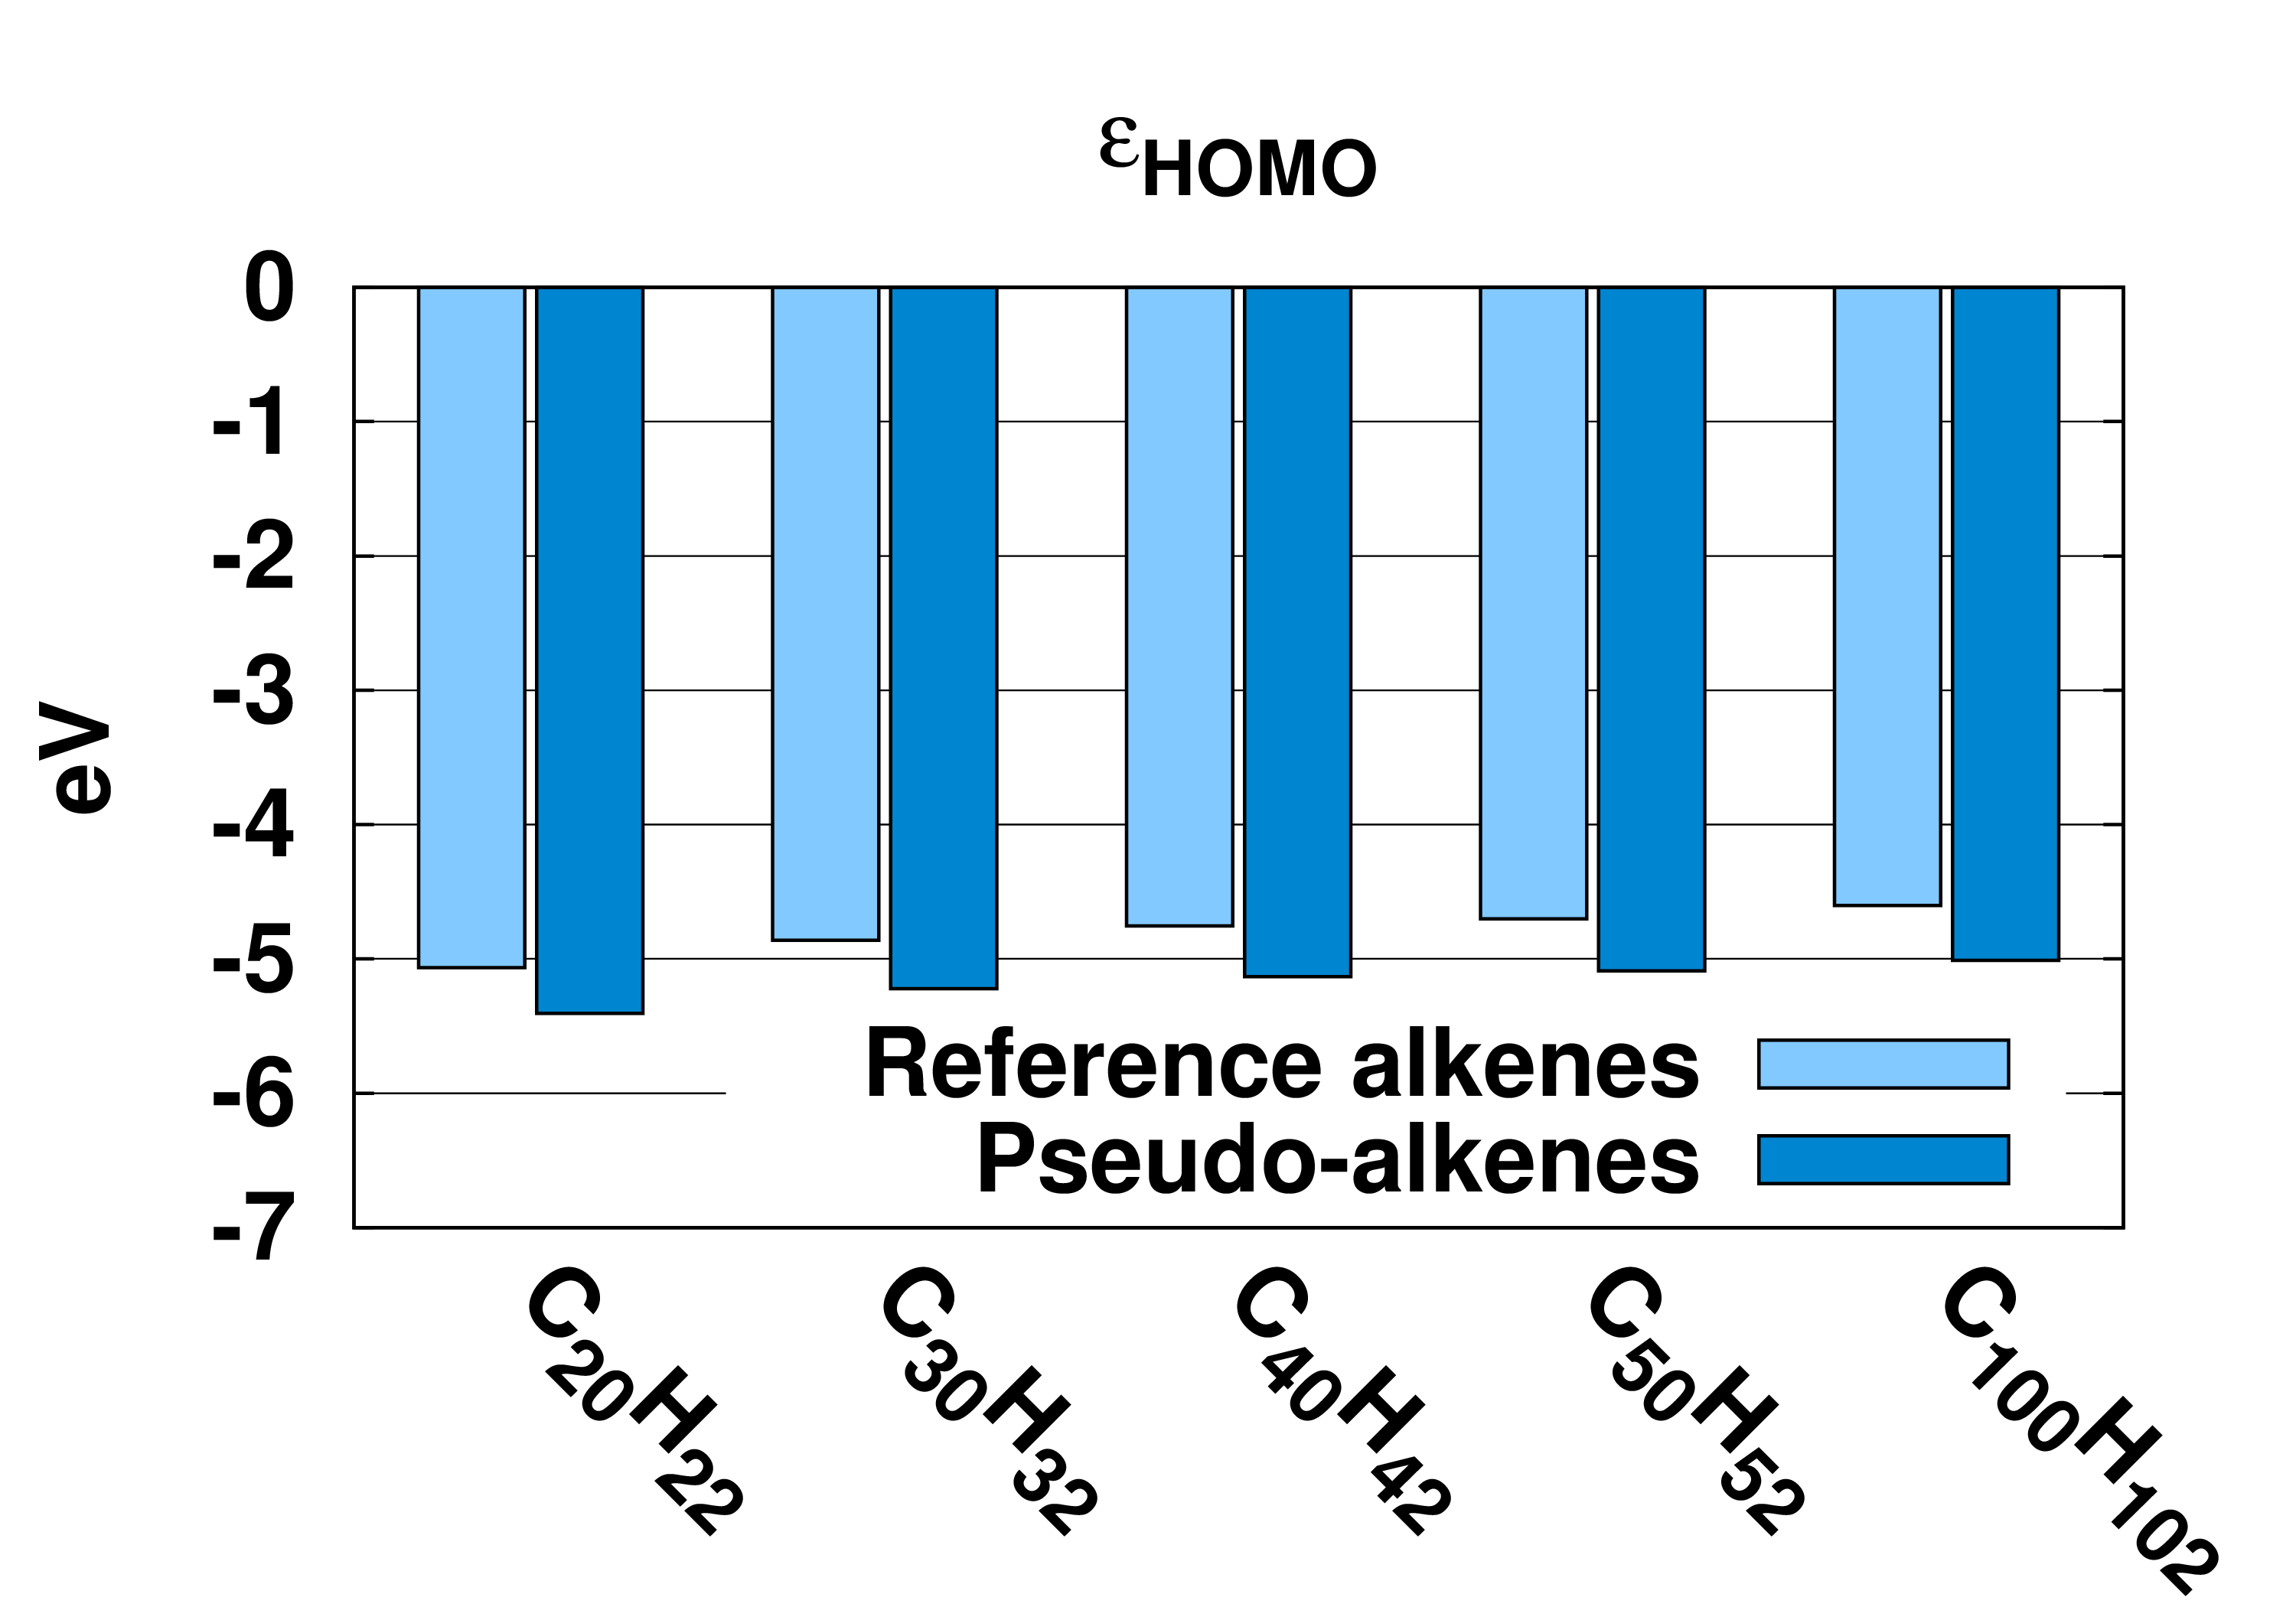
\includegraphics[width=8cm]{long_pbe0_homo}
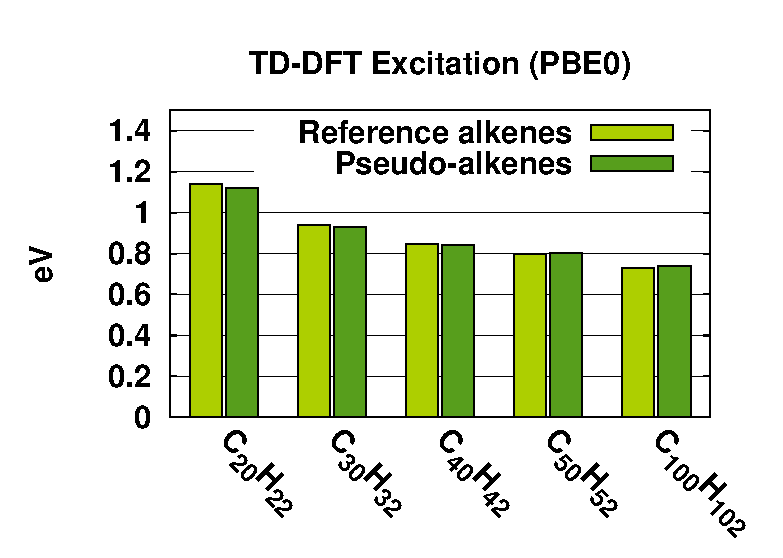
\includegraphics[width=8cm]{long_pbe0_tddft}
%\caption{DFT and TD-DFT (PBE0) comparison of reference and pseudo-system energies across a range of long chain alkenes (C\(_{20}\)-C\(_{100}\)).}
%\label{fig:long_chain_graphs}
\end{center}
\vspace{0.25in}
\hspace*{3in}

\caption{DFT and TD-DFT (PBE0) comparison of reference and pseudo-system energies across a range of long chain alkenes (C\(_{20}\)-C\(_{100}\)).}
\label{fig:long_chain_graphs}
\end{figure}

\begin{figure}
%\vspace*{0.1in}   %%% FIGURE 7
\begin{center}
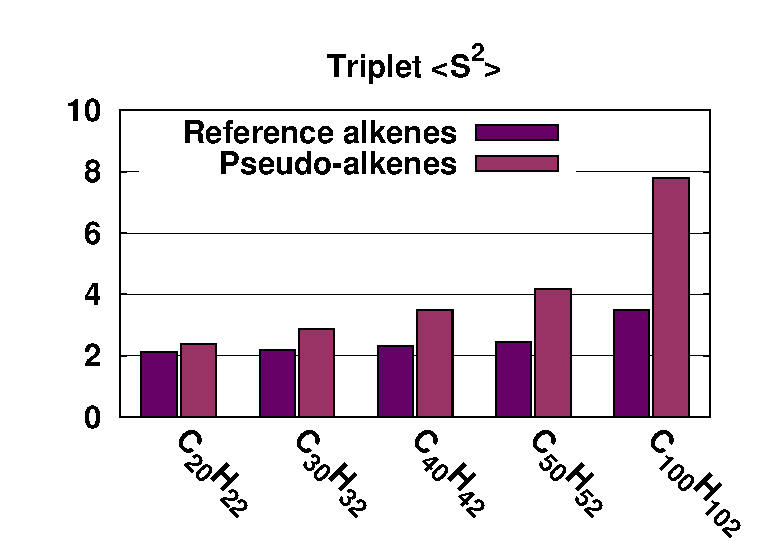
\includegraphics[width=8cm]{long_pbe0_s2}
%\caption{Comparison of $S^2$ expectation values obtained for the calculation
%of the first triplet configuration in a SCF formalism, for reference
%and pseudo-systems.}
%\label{fig:ssquare}
\end{center}
\vspace{0.25in}
\hspace*{3in}
\caption{Comparison of $S^2$ expectation values obtained for the calculation
of the first triplet configuration in a SCF formalism, for reference
and pseudo-systems.}
\label{fig:ssquare}
\end{figure}

%\begin{figure}
%%\vspace*{0.1in}   %%% FIGURE 8
%\begin{center}
%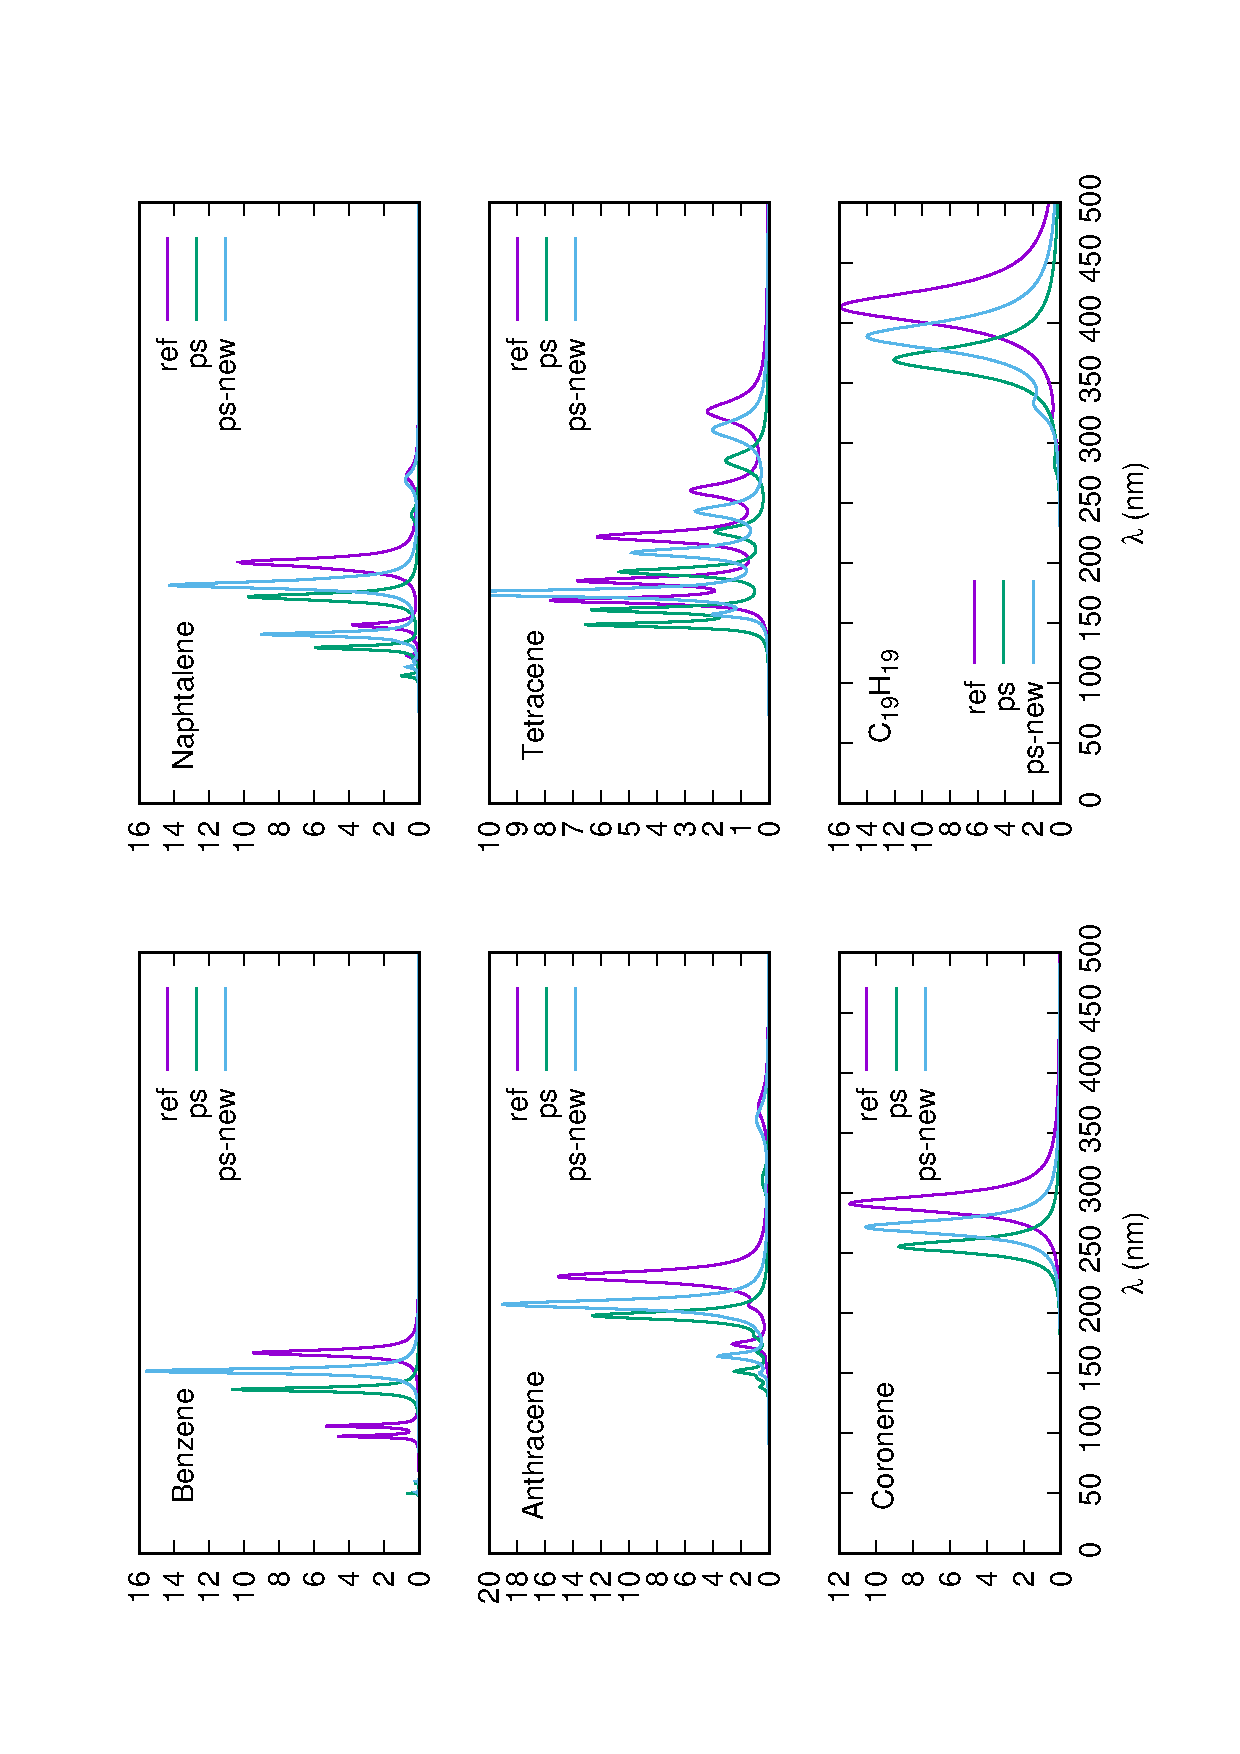
\includegraphics[width=\textwidth]{cnhn_uv}
%\end{center}
%\vspace{0.25in}
%\hspace*{3in}
%\caption{Comparison of the UV spectra obtained with pseudo potentials from the previous section (green), the current section (blue) and reference calculations def2-TZVP/TD-PBE0 (red).}
%\label{fig:cnhn_uv}
%\end{figure}
%%%%%%%%%%%%%%%%%%%%%%%%%%%%

% FIGURES %%%%%%%%%%%%%%%%%%%%%%%%%%%%%%%%%%%%%%%%%%%%%%%%%%%%%%%%%%%%%%%%%%%%%%%%%%%%%%%%%
% FIGURES % FIGURE FILES
% FIGURES 
% FIGURES \clearpage
% FIGURES 
% FIGURES %\vspace*{0.1in}   %%% FIGURE 1
% FIGURES \begin{center}
% FIGURES %\includegraphics[width=0.2\columnwidth,keepaspectratio=true]{cc.eps}
% FIGURES 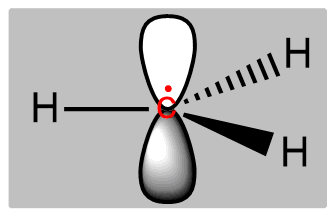
\includegraphics[width=8cm]{ch3.png}
% FIGURES 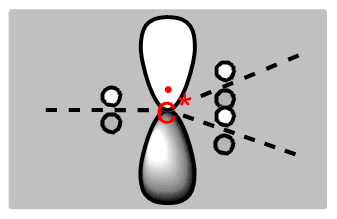
\includegraphics[width=8cm]{pseudoch3.png}
% FIGURES 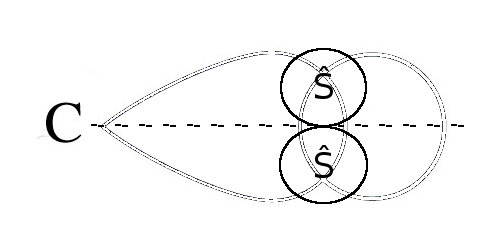
\includegraphics[width=8cm]{tm_sp2_potentials.png}
% FIGURES %\caption{Diagrams of CH\(^{\bullet}_{3}\) (left) and pseudo-CH\(^{\bullet}_{3}\) (right, below) molecules. The pseudo-CH\(^{\bullet}_{3}\) diagrams display the \(s\) and \(p\)-potential positions, and the distances \(d\) and \(c\).}
% FIGURES %\label{figure:ref_pseudo_diagram}
% FIGURES \end{center}
% FIGURES \vspace{0.25in}
% FIGURES \hspace*{3in}
% FIGURES {\Large
% FIGURES \begin{minipage}[t]{3in}
% FIGURES \baselineskip = .5\baselineskip
% FIGURES Figure 1 \\
% FIGURES Alexander Punter, Paola Nava, Yannick Carissan \\
% FIGURES J.\ Comput.\ Chem.
% FIGURES \end{minipage}
% FIGURES }
% FIGURES 
% FIGURES \clearpage
% FIGURES 
% FIGURES %\vspace*{0.1in}   %%% FIGURE 2
% FIGURES \begin{center}
% FIGURES %\includegraphics[width=0.2\columnwidth,keepaspectratio=true]{cc.eps}
% FIGURES \fbox{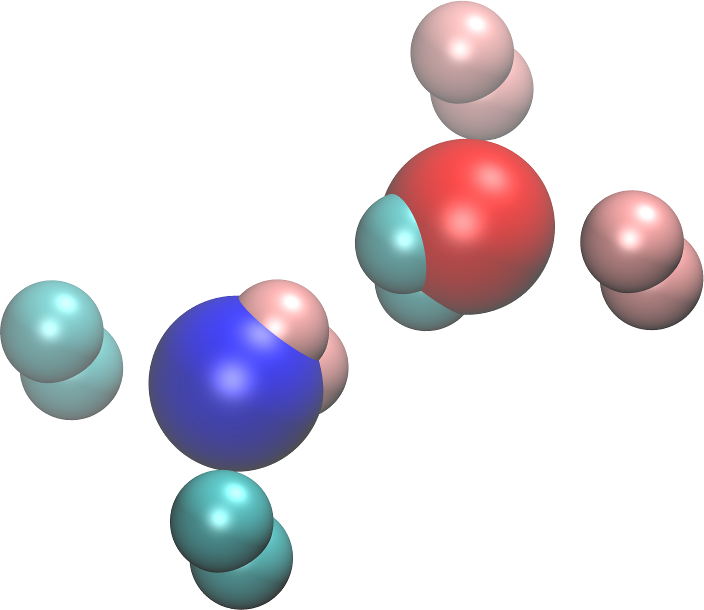
\includegraphics[width=0.45\textwidth]{hires_long_r_crop.png}}%
% FIGURES \fbox{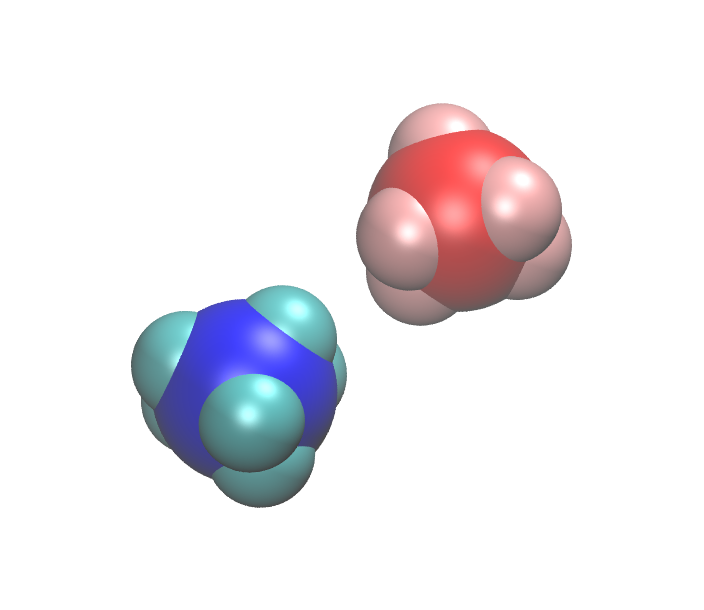
\includegraphics[width=0.45\textwidth]{hires_short_r_crop.png}}
% FIGURES %\caption{Diagrams of pseudo-ethene with \(d =\) 2.0 a.u. (left), and \(d = 0.5\) a.u. (right). The first pseudo-carbon is displayed in blue, with its \(s\) pseudo-potentials in cyan, and the second pseudo-carbon is in red, with its potentials in pink.}
% FIGURES %\label{fig:long_r_ethene}
% FIGURES \end{center}
% FIGURES \vspace{0.25in}
% FIGURES \hspace*{3in}
% FIGURES {\Large
% FIGURES \begin{minipage}[t]{3in}
% FIGURES \baselineskip = .5\baselineskip
% FIGURES Figure 2 \\
% FIGURES Alexander Punter, Paola Nava, Yannick Carissan \\
% FIGURES J.\ Comput.\ Chem.
% FIGURES \end{minipage}
% FIGURES }
% FIGURES 
% FIGURES \clearpage
% FIGURES 
% FIGURES %\vspace*{0.1in}   %%% FIGURE 3
% FIGURES \begin{center}
% FIGURES 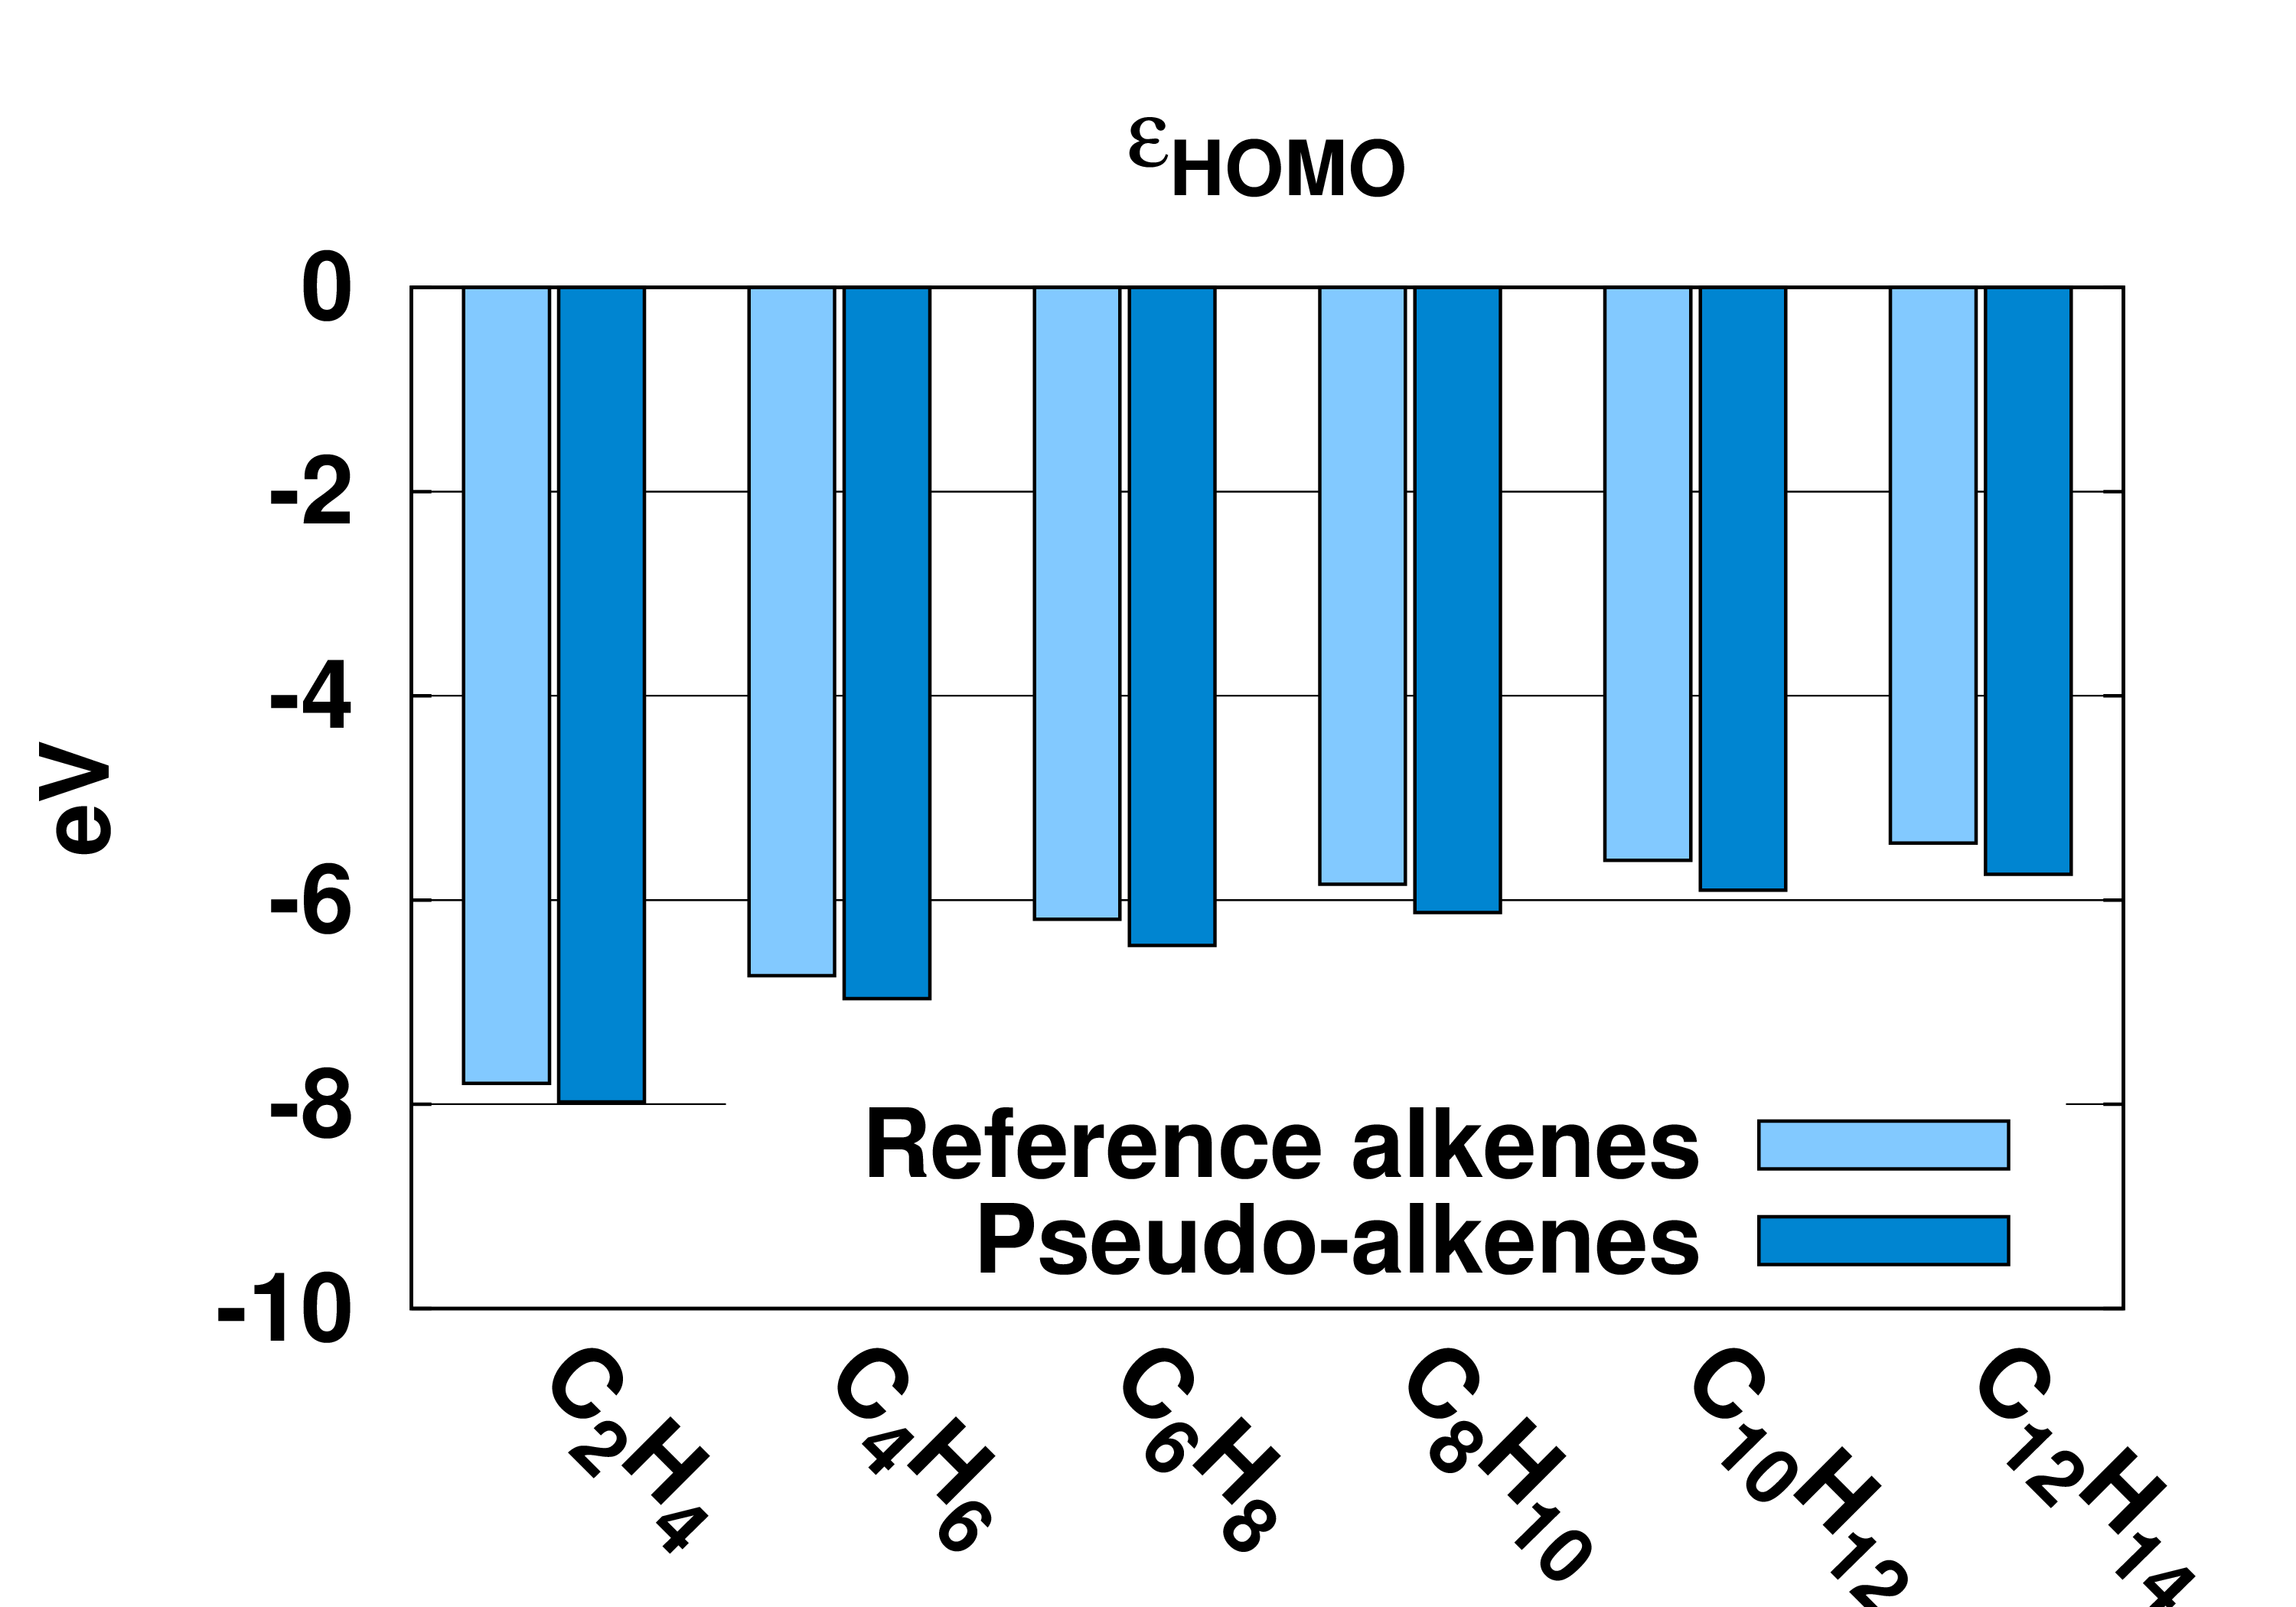
\includegraphics[width=8cm]{short_pbe0_homo}
% FIGURES 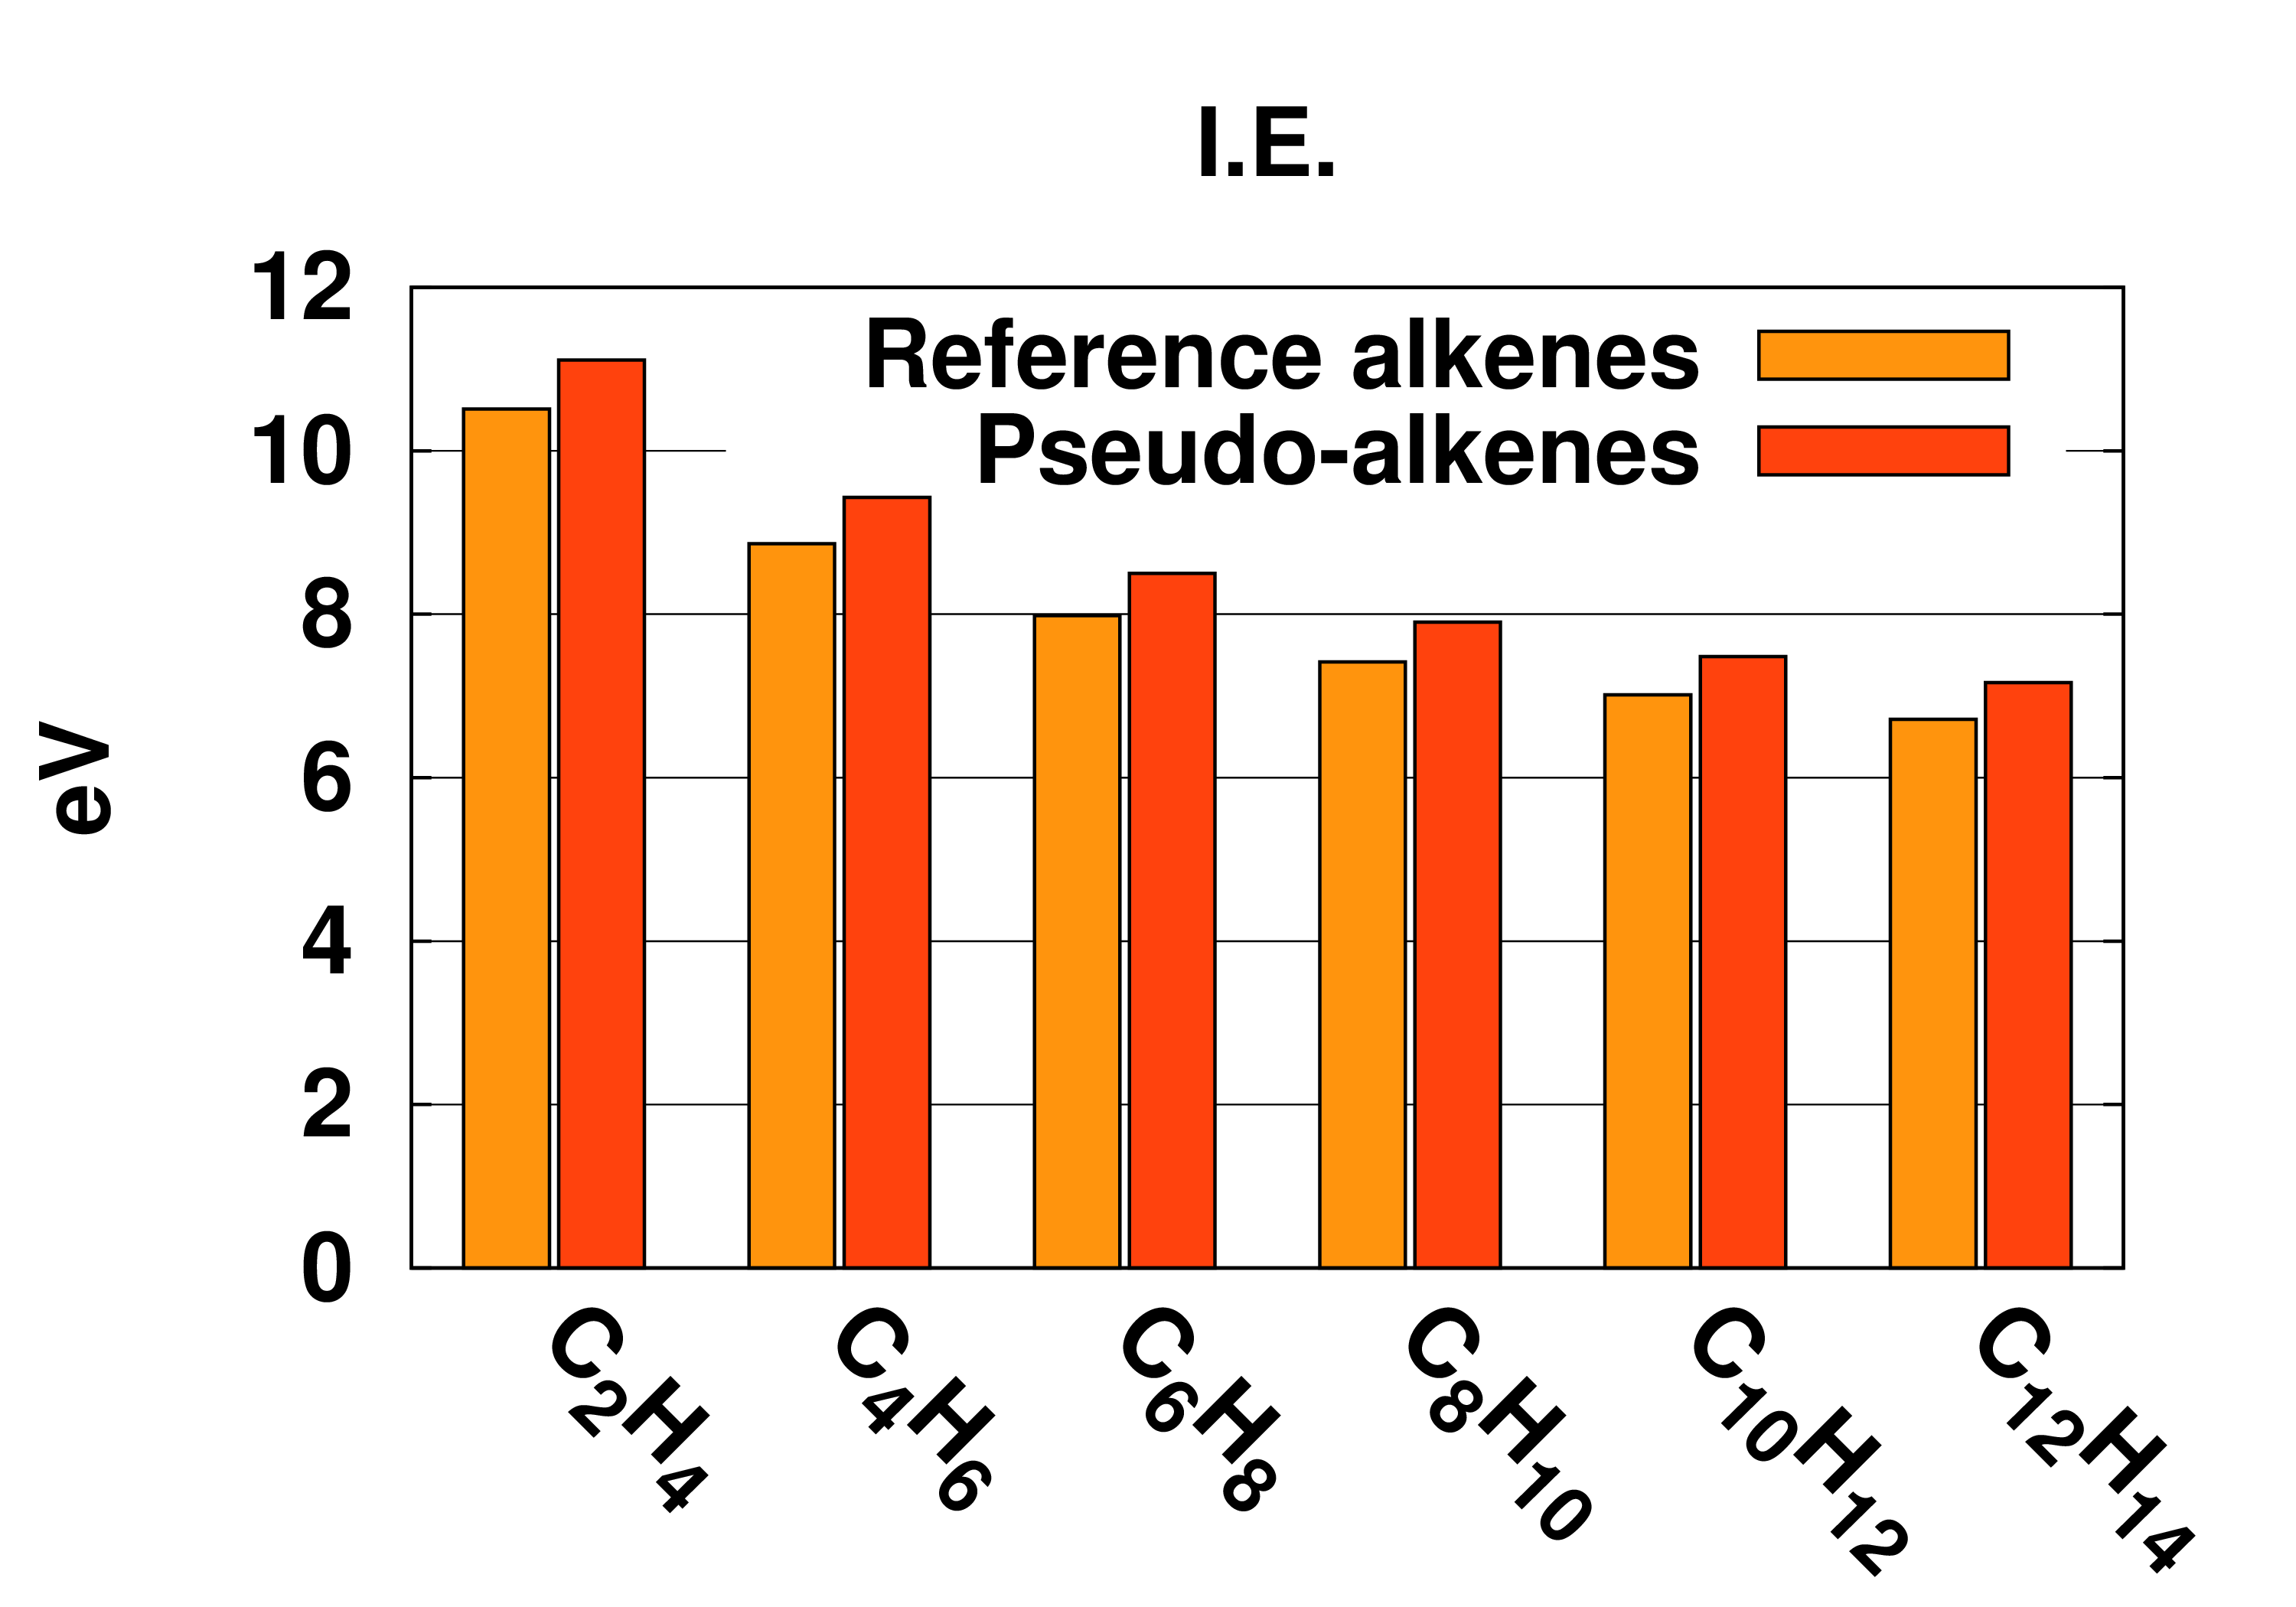
\includegraphics[width=8cm]{short_pbe0_ie}
% FIGURES 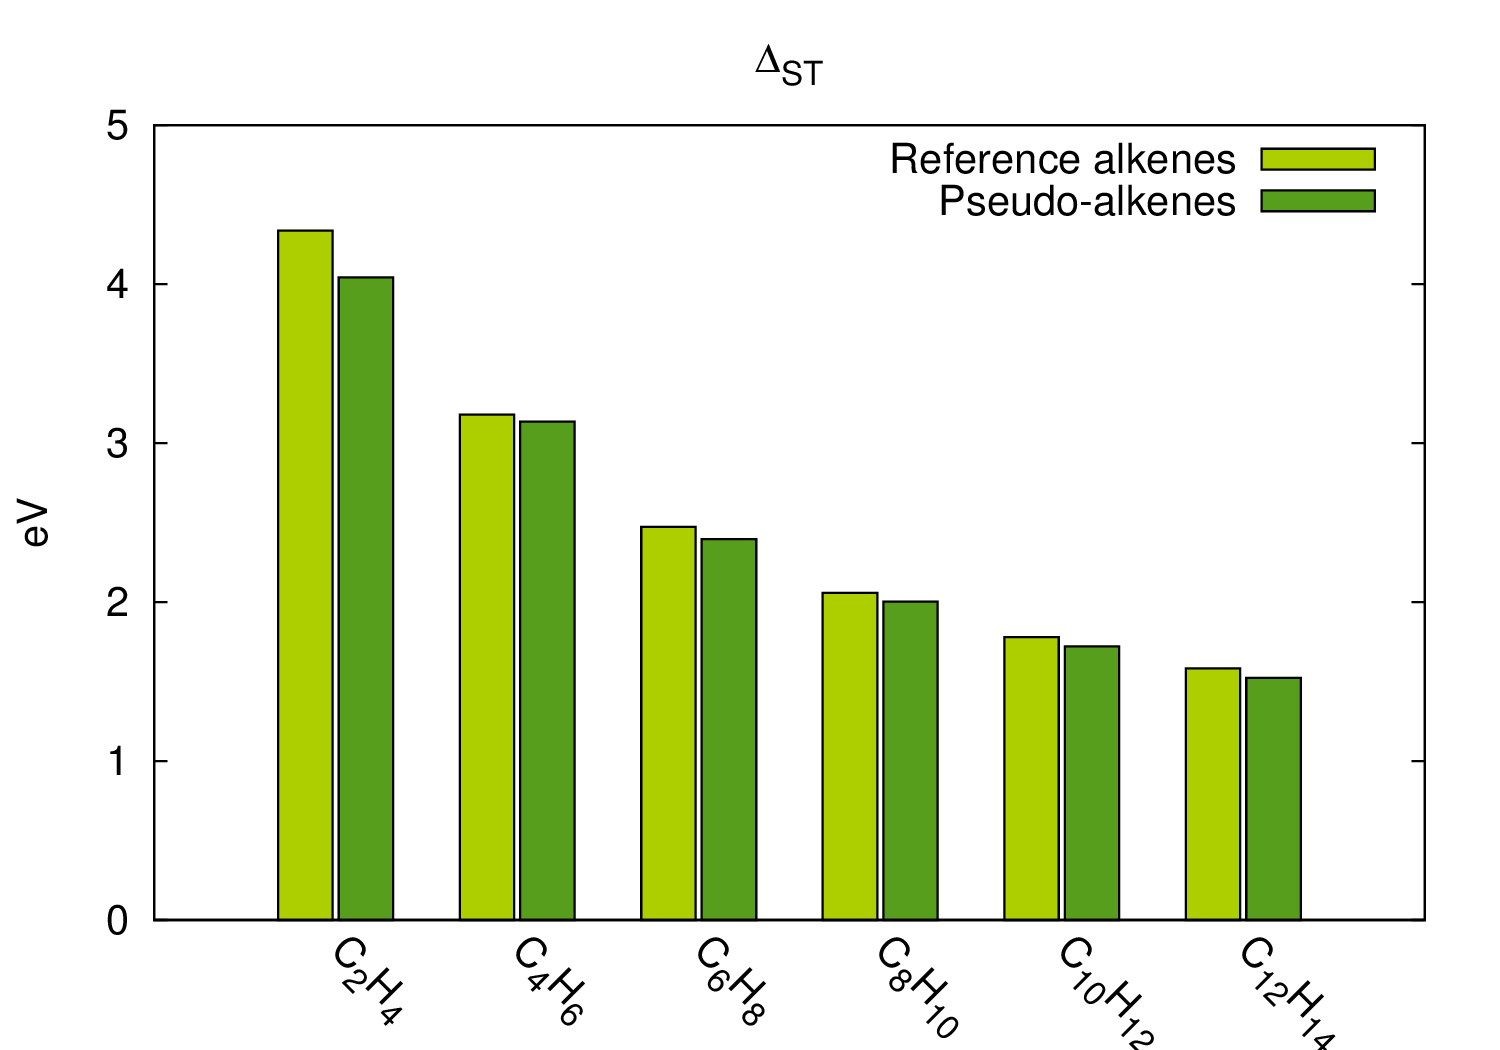
\includegraphics[width=8cm]{short_pbe0_st}
% FIGURES %\caption{DFT (PBE0) comparison of reference and pseudo-system energies across a range of chain alkenes.}
% FIGURES %\label{fig:alkenes_hf_dft}
% FIGURES \end{center}
% FIGURES \vspace{0.25in}
% FIGURES \hspace*{3in}
% FIGURES {\Large
% FIGURES \begin{minipage}[t]{3in}
% FIGURES \baselineskip = .5\baselineskip
% FIGURES Figure 3 \\
% FIGURES Alexander Punter, Paola Nava, Yannick Carissan \\
% FIGURES J.\ Comput.\ Chem.
% FIGURES \end{minipage}
% FIGURES }
% FIGURES 
% FIGURES \clearpage
% FIGURES 
% FIGURES %\vspace*{0.1in}   %%% FIGURE 4
% FIGURES \begin{center}
% FIGURES 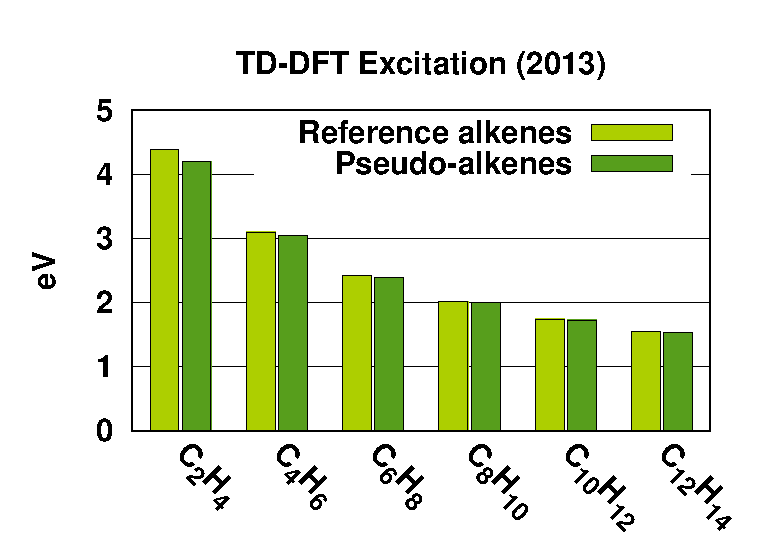
\includegraphics[width=8cm]{short_pbe0_tddft_2013}
% FIGURES 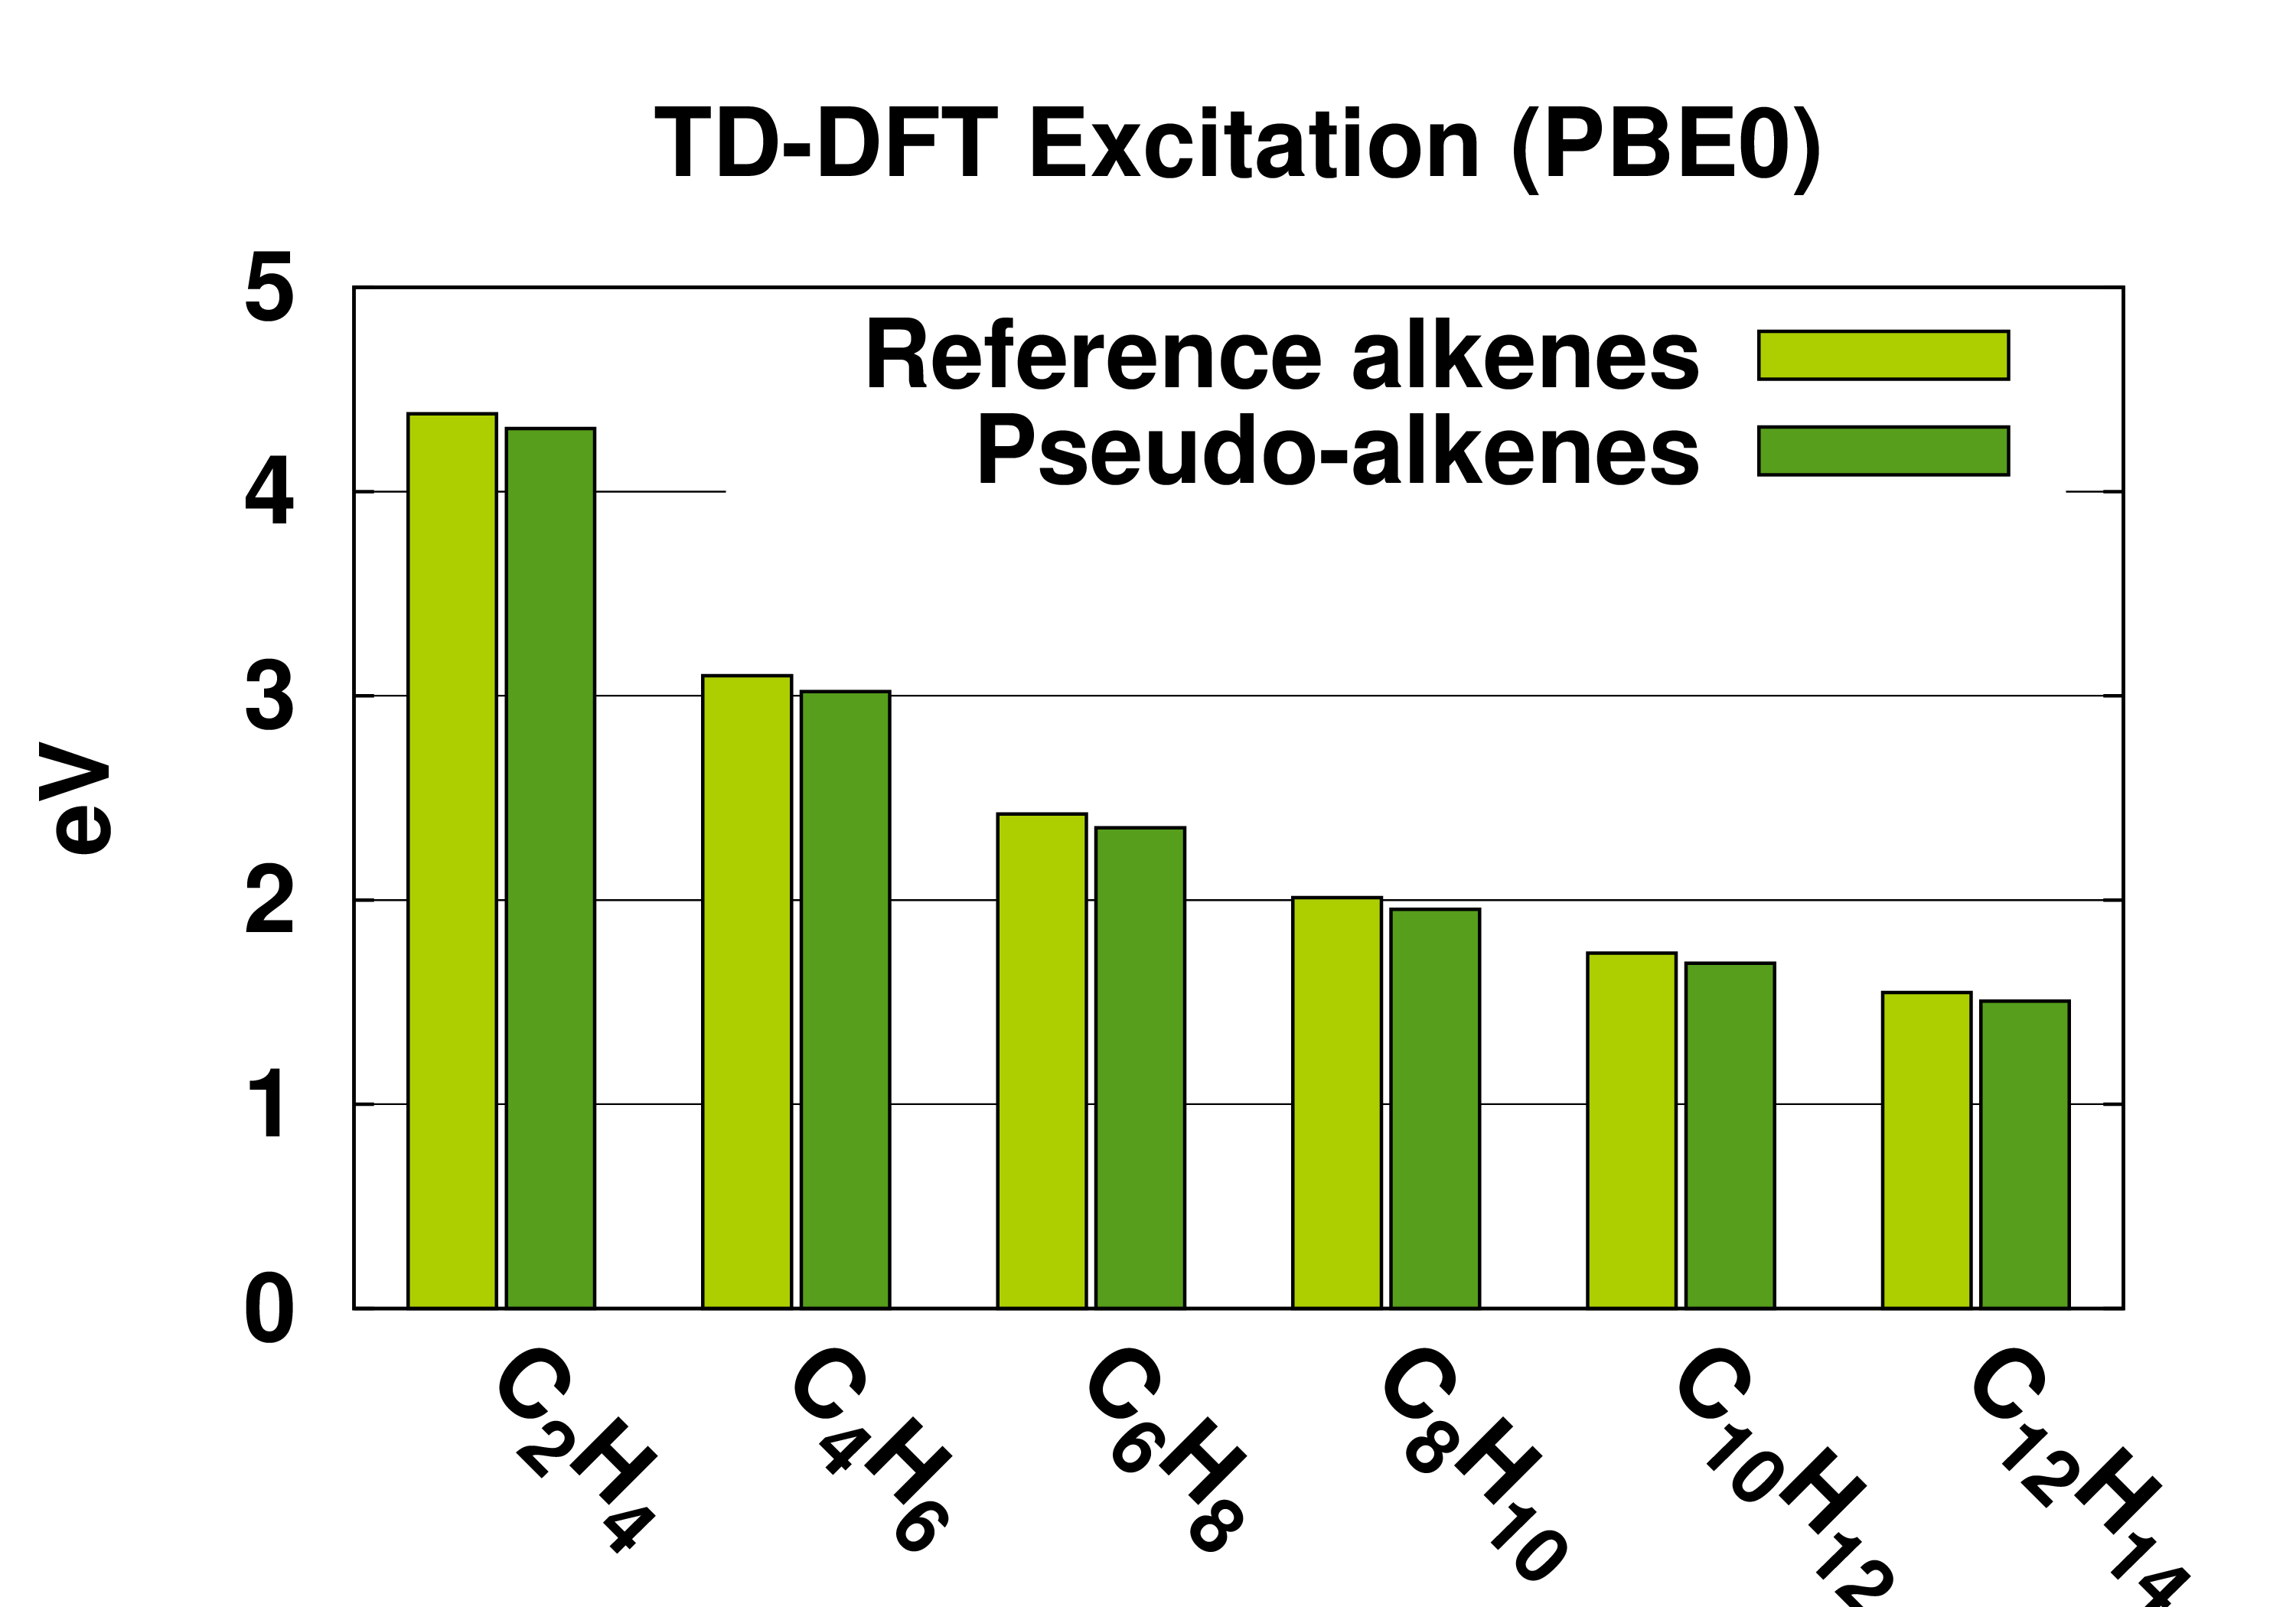
\includegraphics[width=8cm]{short_pbe0_tddft}
% FIGURES %\caption{Comparison of pseudo-alkenes with previous\cite{drujon_pseudopotentials_2013} and current potentials using TD-DFT excitation energies.}
% FIGURES %\label{fig:alkenes_tddft}
% FIGURES \end{center}
% FIGURES \vspace{0.25in}
% FIGURES \hspace*{3in}
% FIGURES {\Large
% FIGURES \begin{minipage}[t]{3in}
% FIGURES \baselineskip = .5\baselineskip
% FIGURES Figure 4 \\
% FIGURES Alexander Punter, Paola Nava, Yannick Carissan \\
% FIGURES J.\ Comput.\ Chem.
% FIGURES \end{minipage}
% FIGURES }
% FIGURES 
% FIGURES \clearpage
% FIGURES 
% FIGURES %\vspace*{0.1in}   %%% FIGURE 5
% FIGURES \begin{center}
% FIGURES 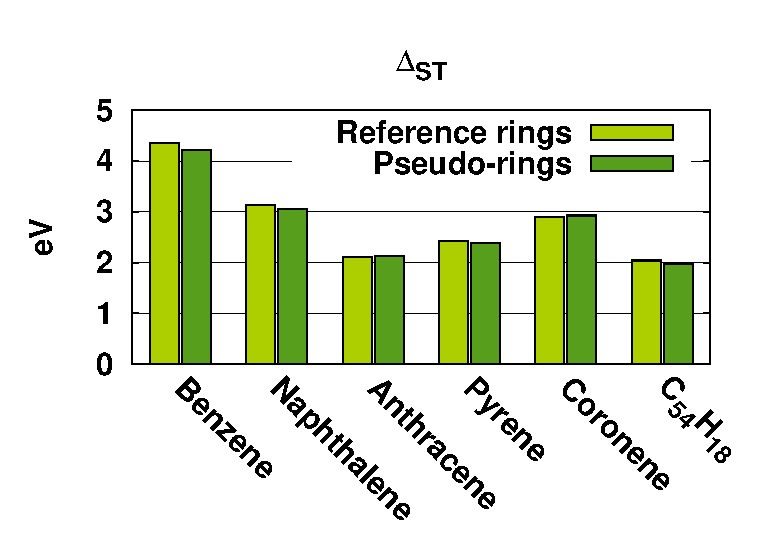
\includegraphics[width=8cm]{ring_pbe0_st}
% FIGURES 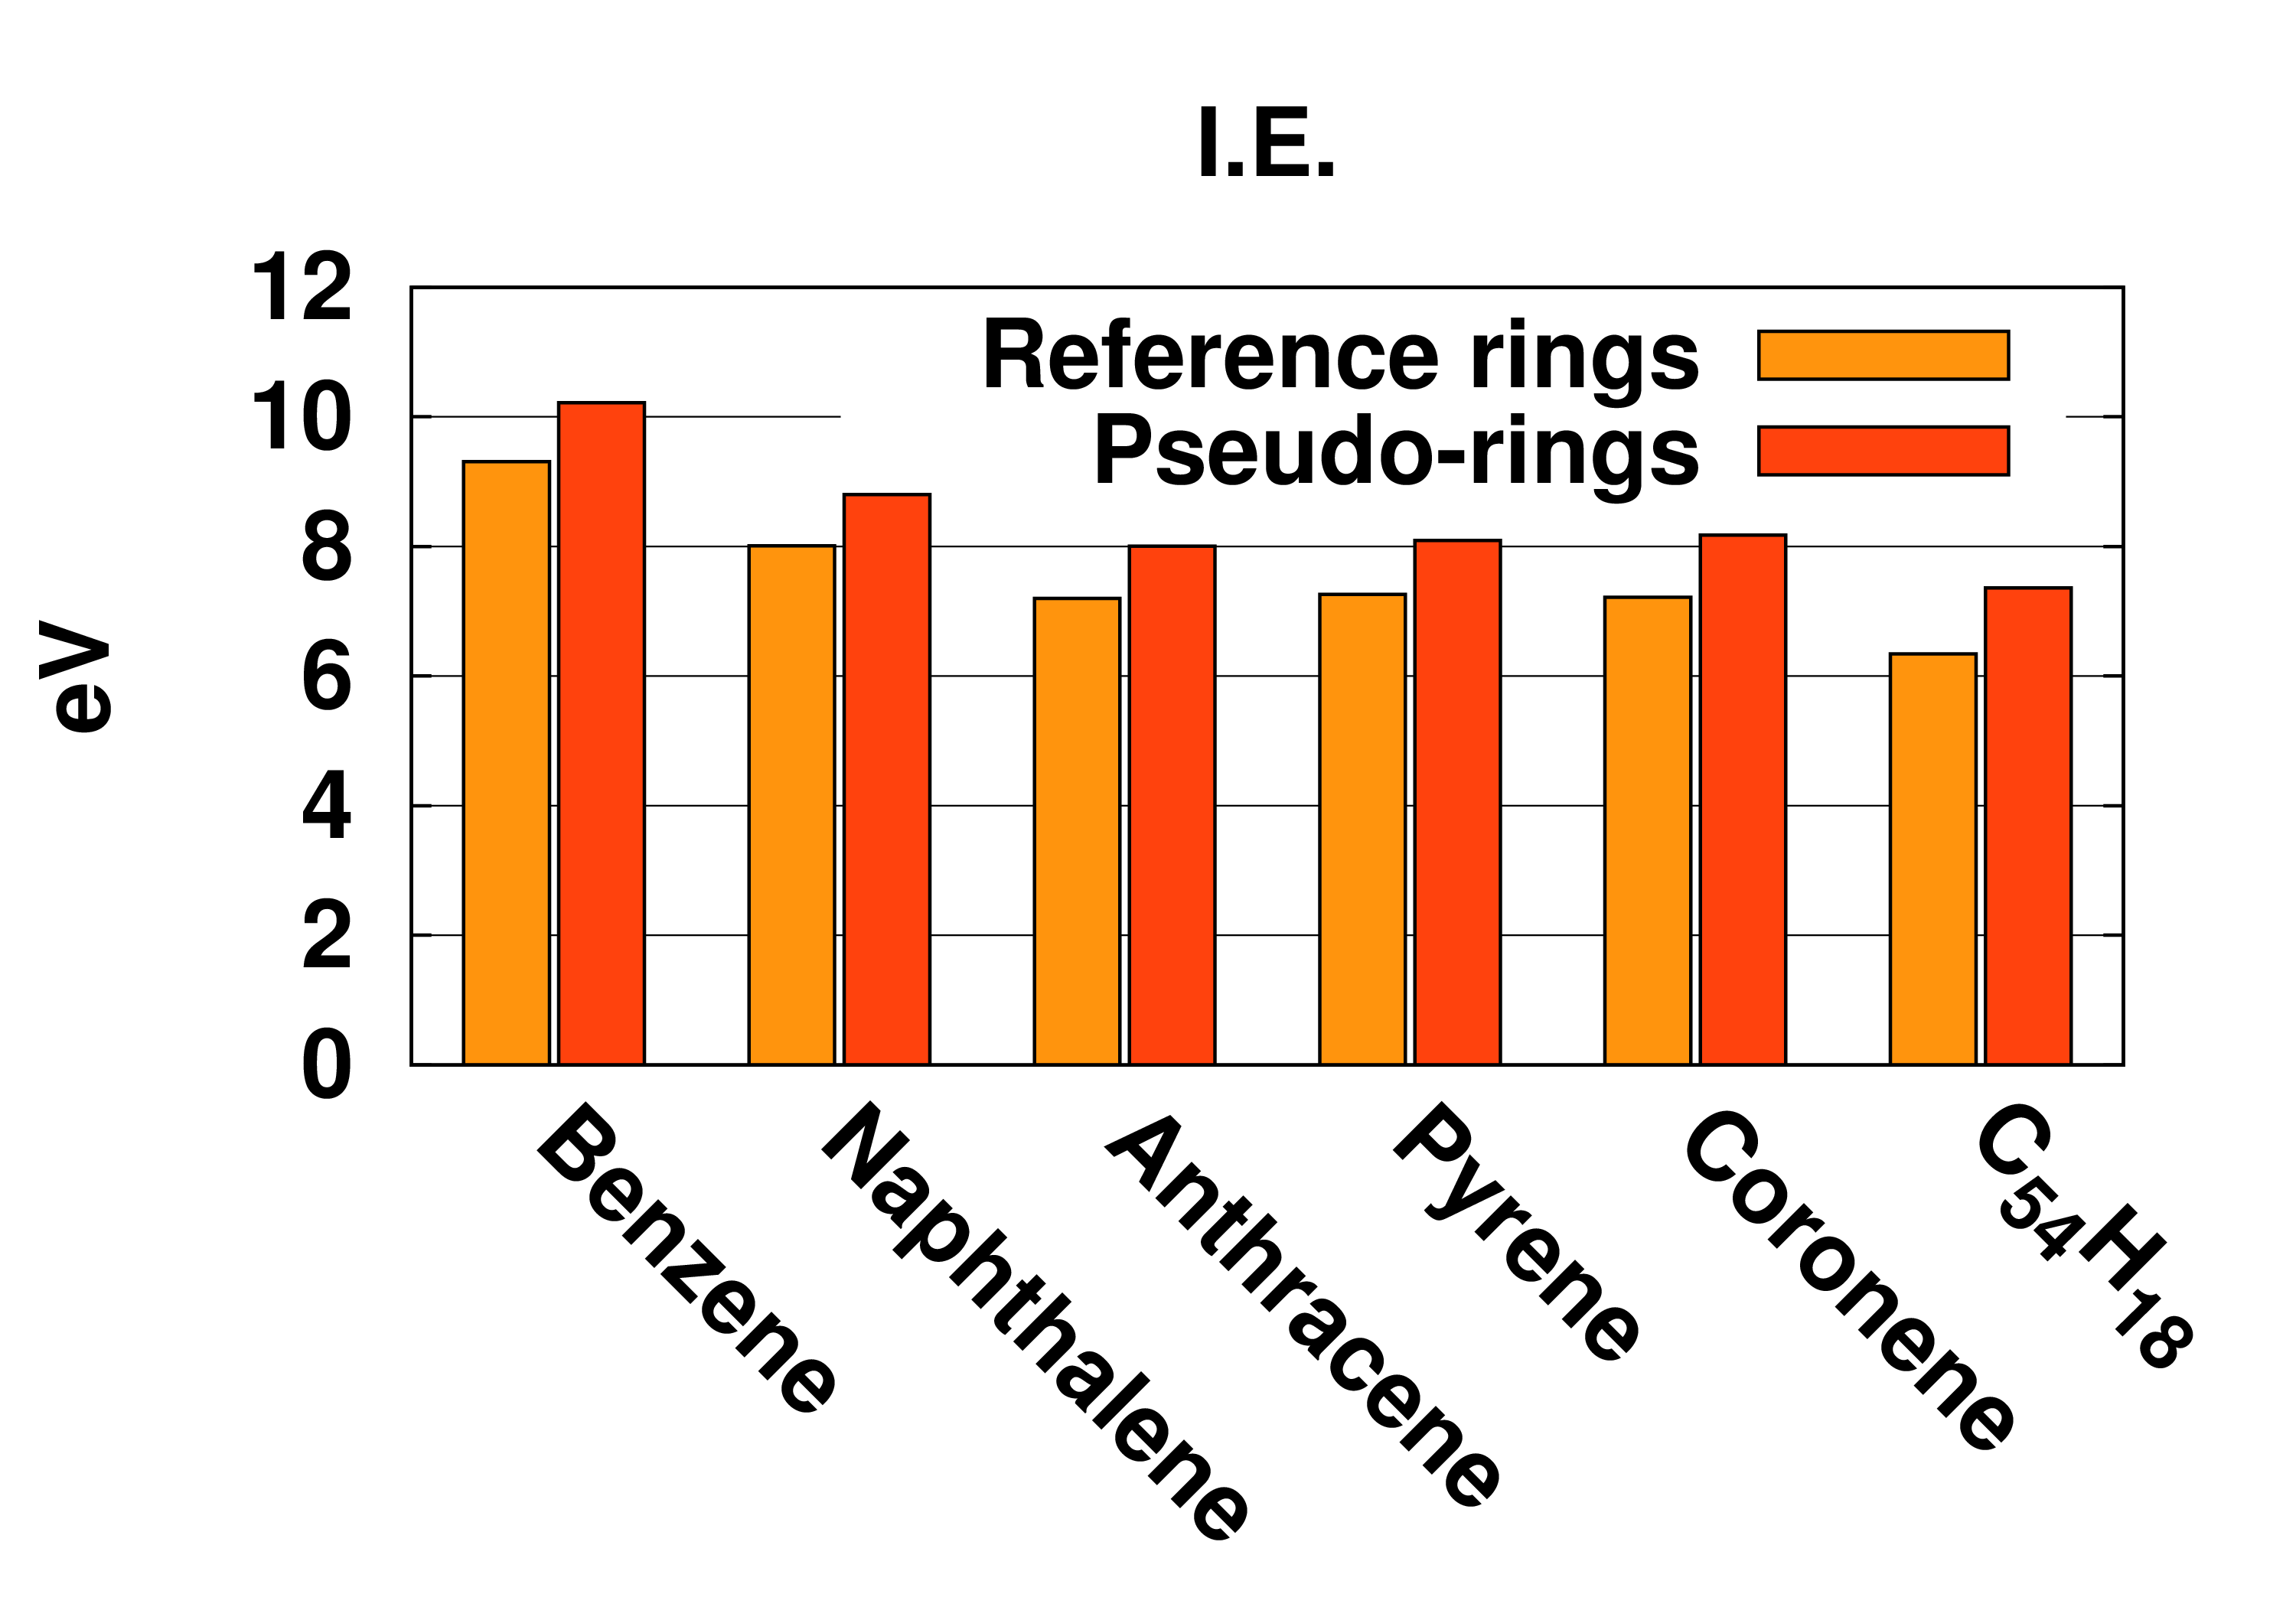
\includegraphics[width=8cm]{ring_pbe0_ie}
% FIGURES 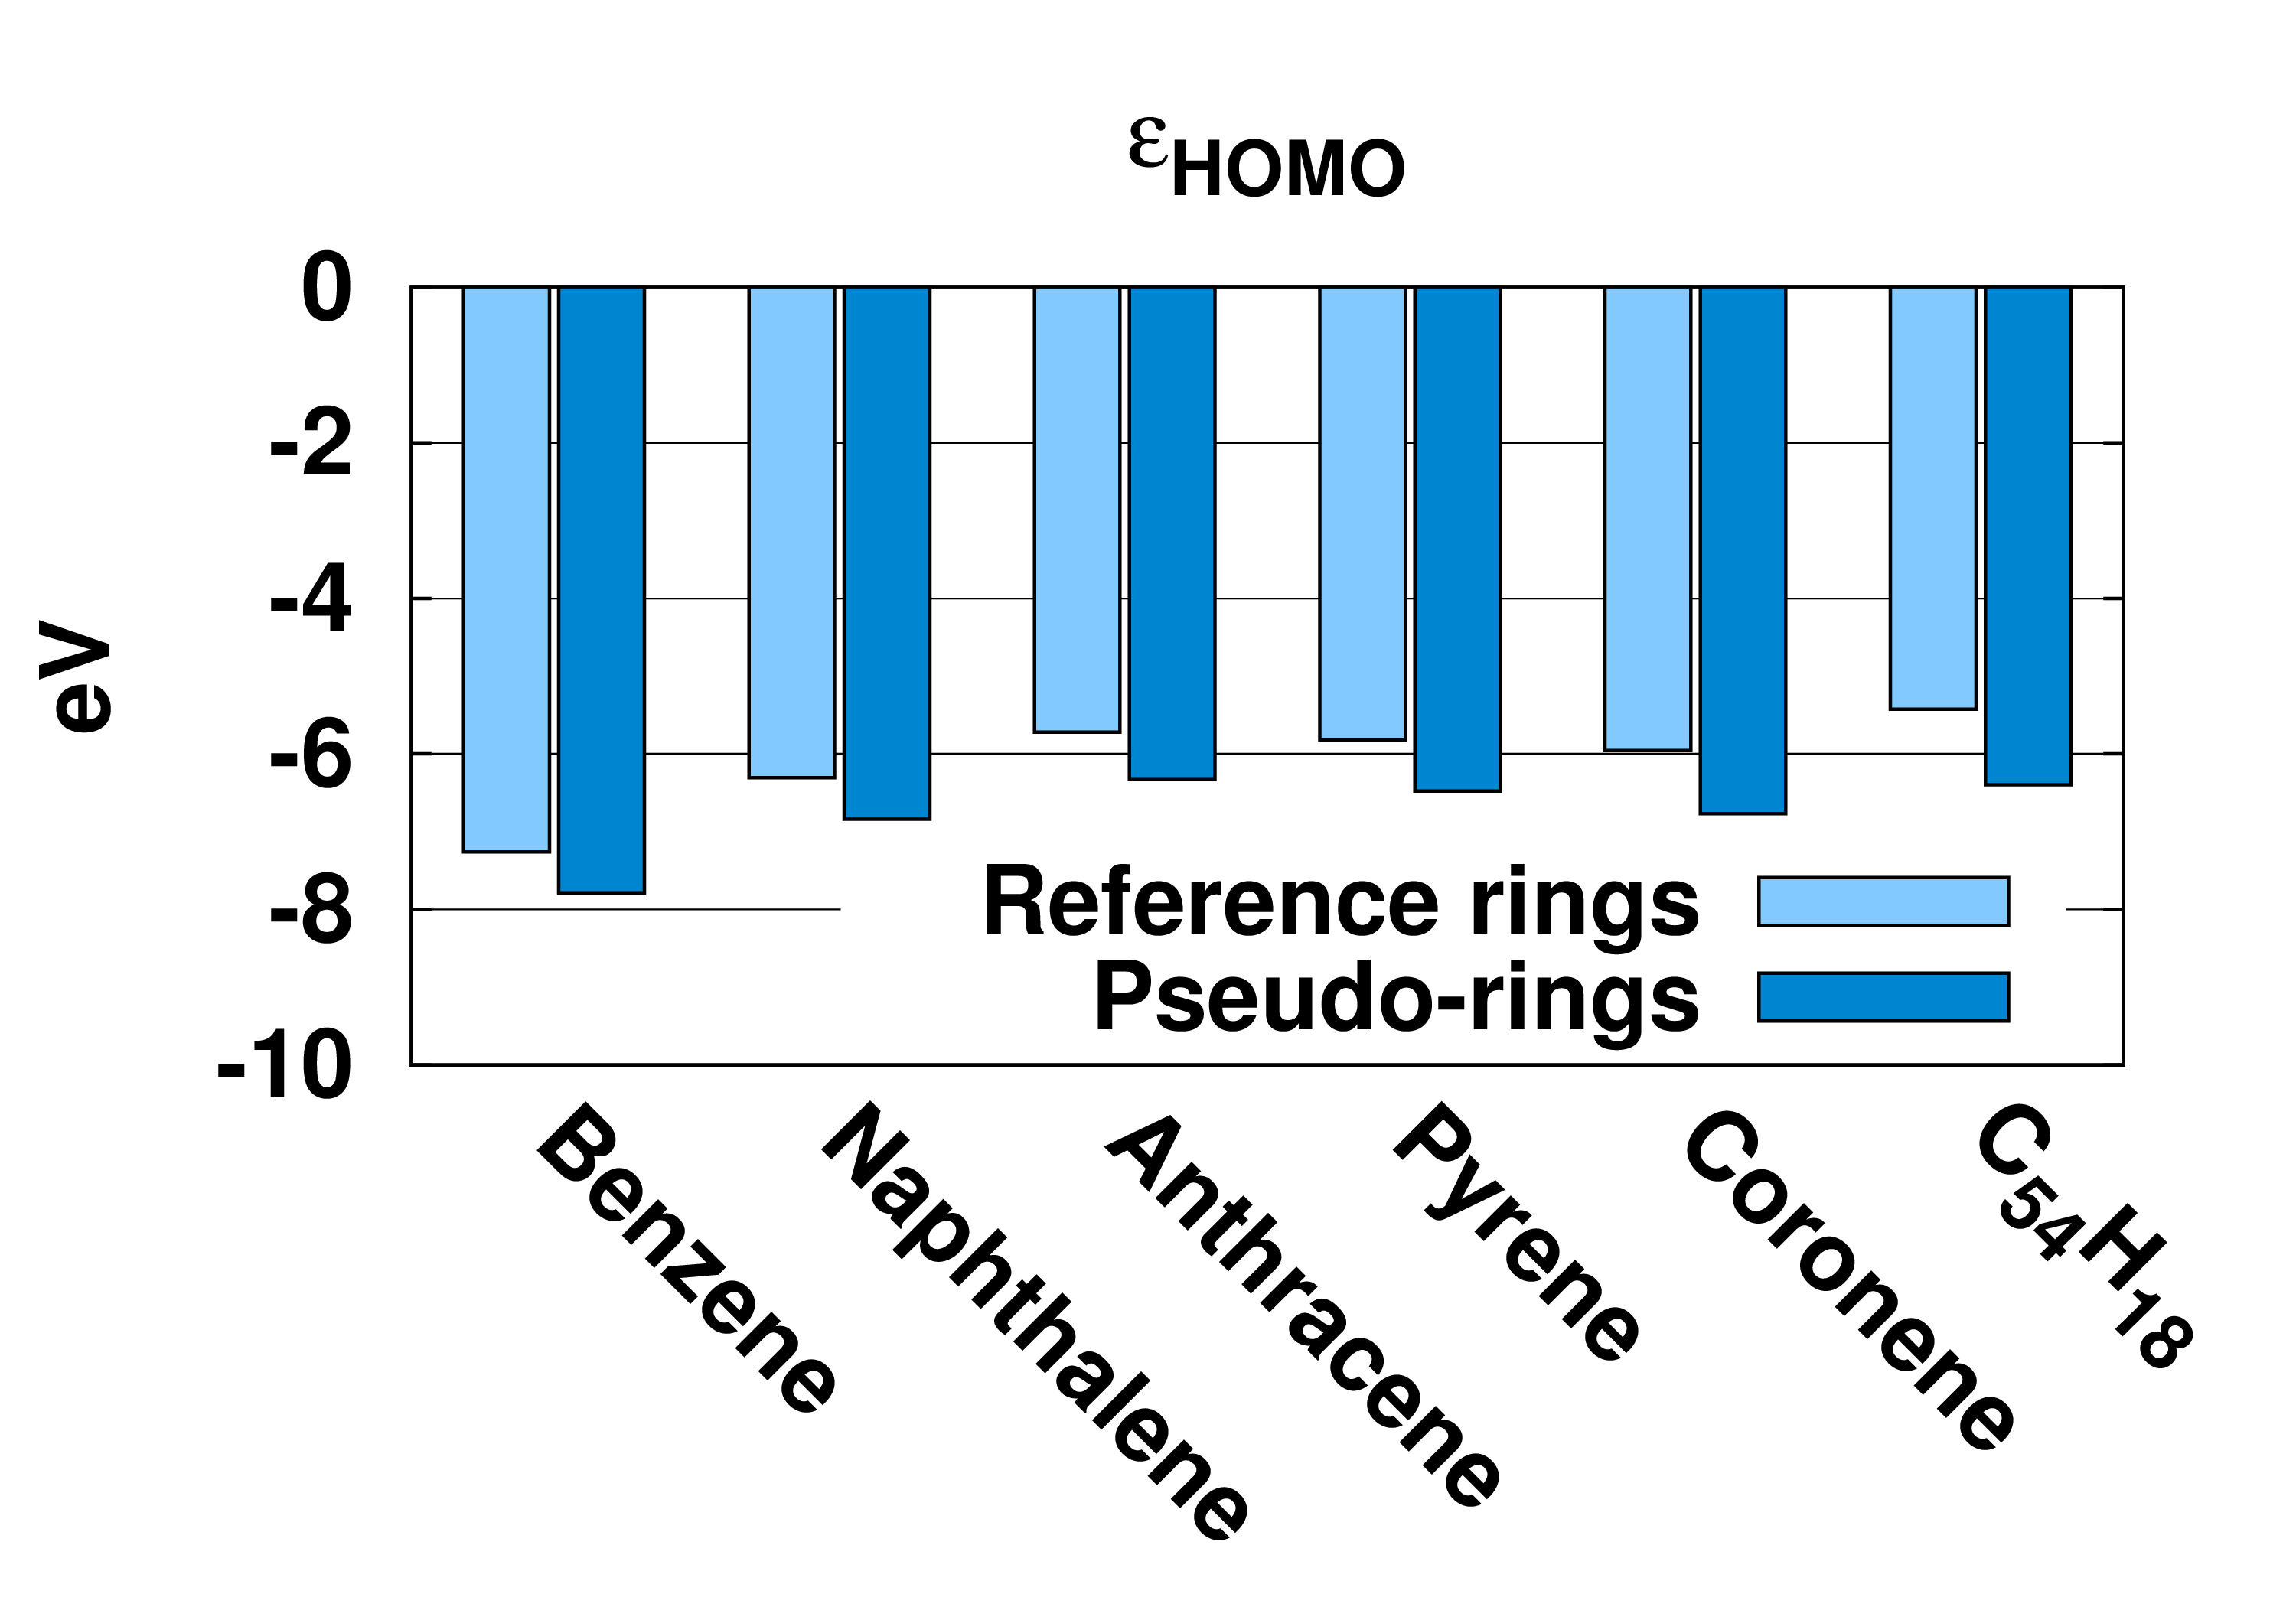
\includegraphics[width=8cm]{ring_pbe0_homo}
% FIGURES 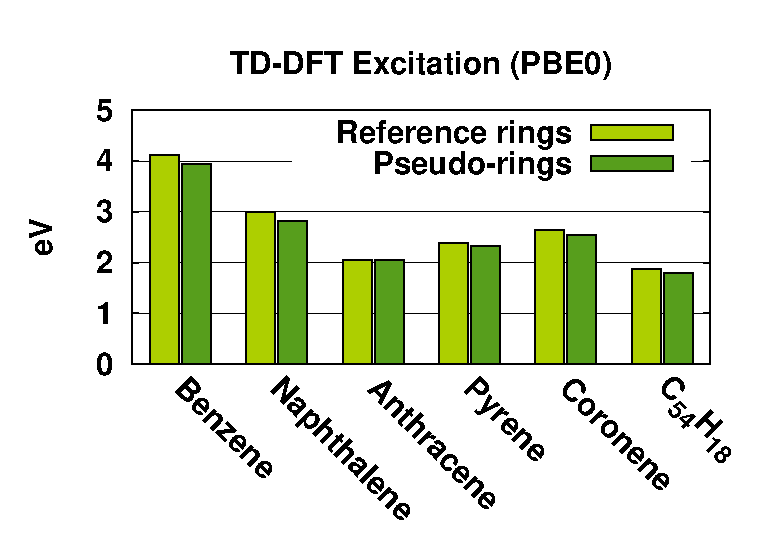
\includegraphics[width=8cm]{ring_pbe0_tddft}
% FIGURES %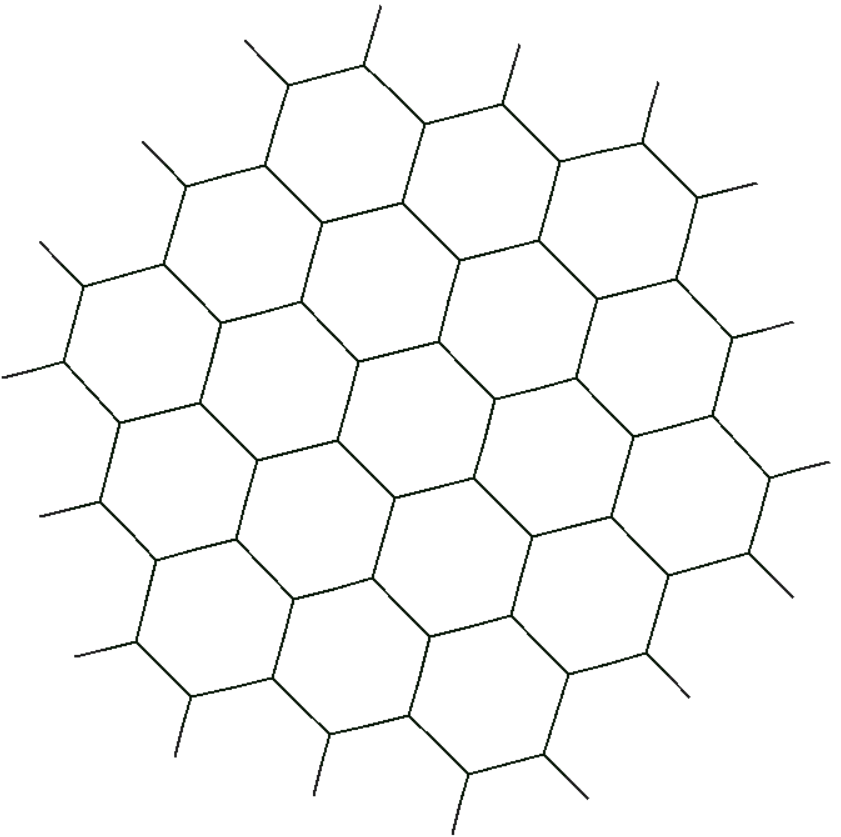
\includegraphics[width=5cm]{19_ring_diagram}
% FIGURES \fbox{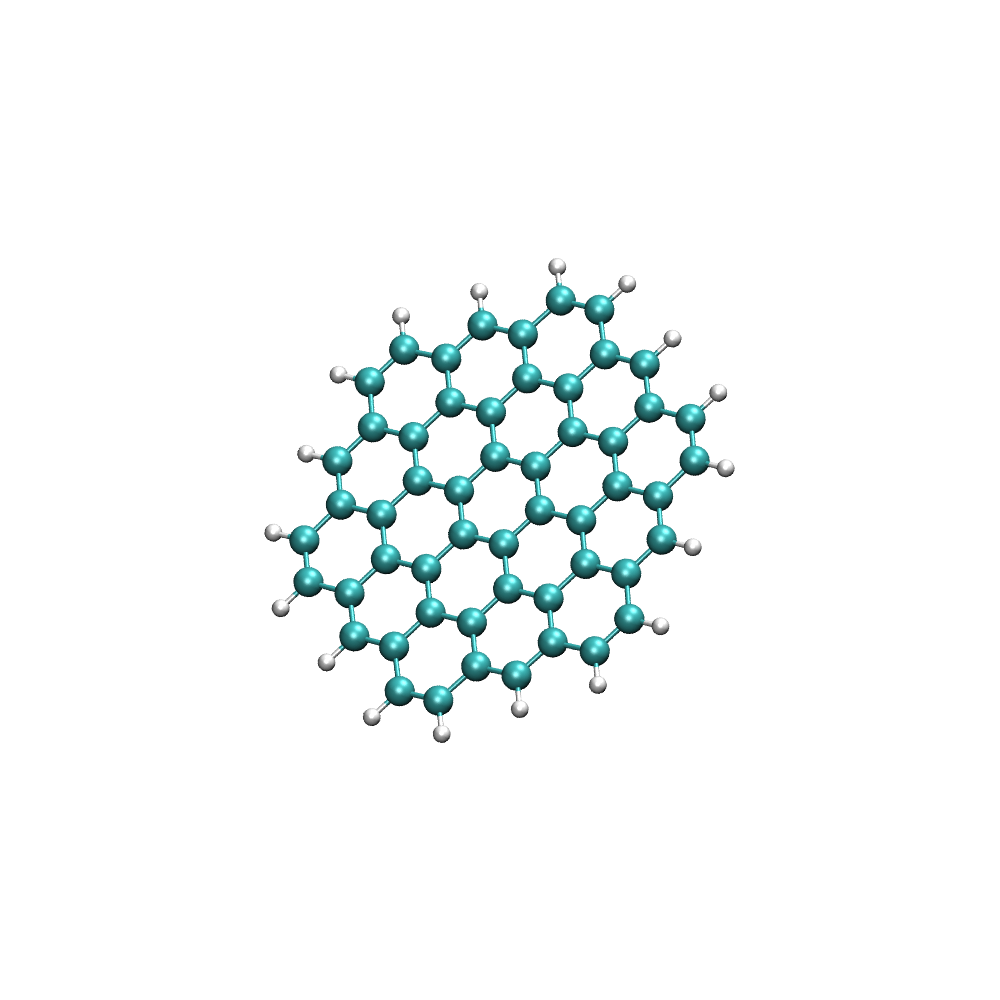
\includegraphics[width=5cm]{c54h18}}
% FIGURES %\caption{DFT and TD-DFT (PBE0) comparison of reference and pseudo-system energies across a range of ring molecules. 
% FIGURES %C\(_{54}\)H\(_{18}\) is shown in the bottom.}
% FIGURES %\label{fig:rings_graphs}
% FIGURES \end{center}
% FIGURES \vspace{0.25in}
% FIGURES \hspace*{3in}
% FIGURES {\Large
% FIGURES \begin{minipage}[t]{3in}
% FIGURES \baselineskip = .5\baselineskip
% FIGURES Figure 5 \\
% FIGURES Alexander Punter, Paola Nava, Yannick Carissan \\
% FIGURES J.\ Comput.\ Chem.
% FIGURES \end{minipage}
% FIGURES }
% FIGURES 
% FIGURES \clearpage
% FIGURES 
% FIGURES %\vspace*{0.1in}   %%% FIGURE 6
% FIGURES \begin{center}
% FIGURES 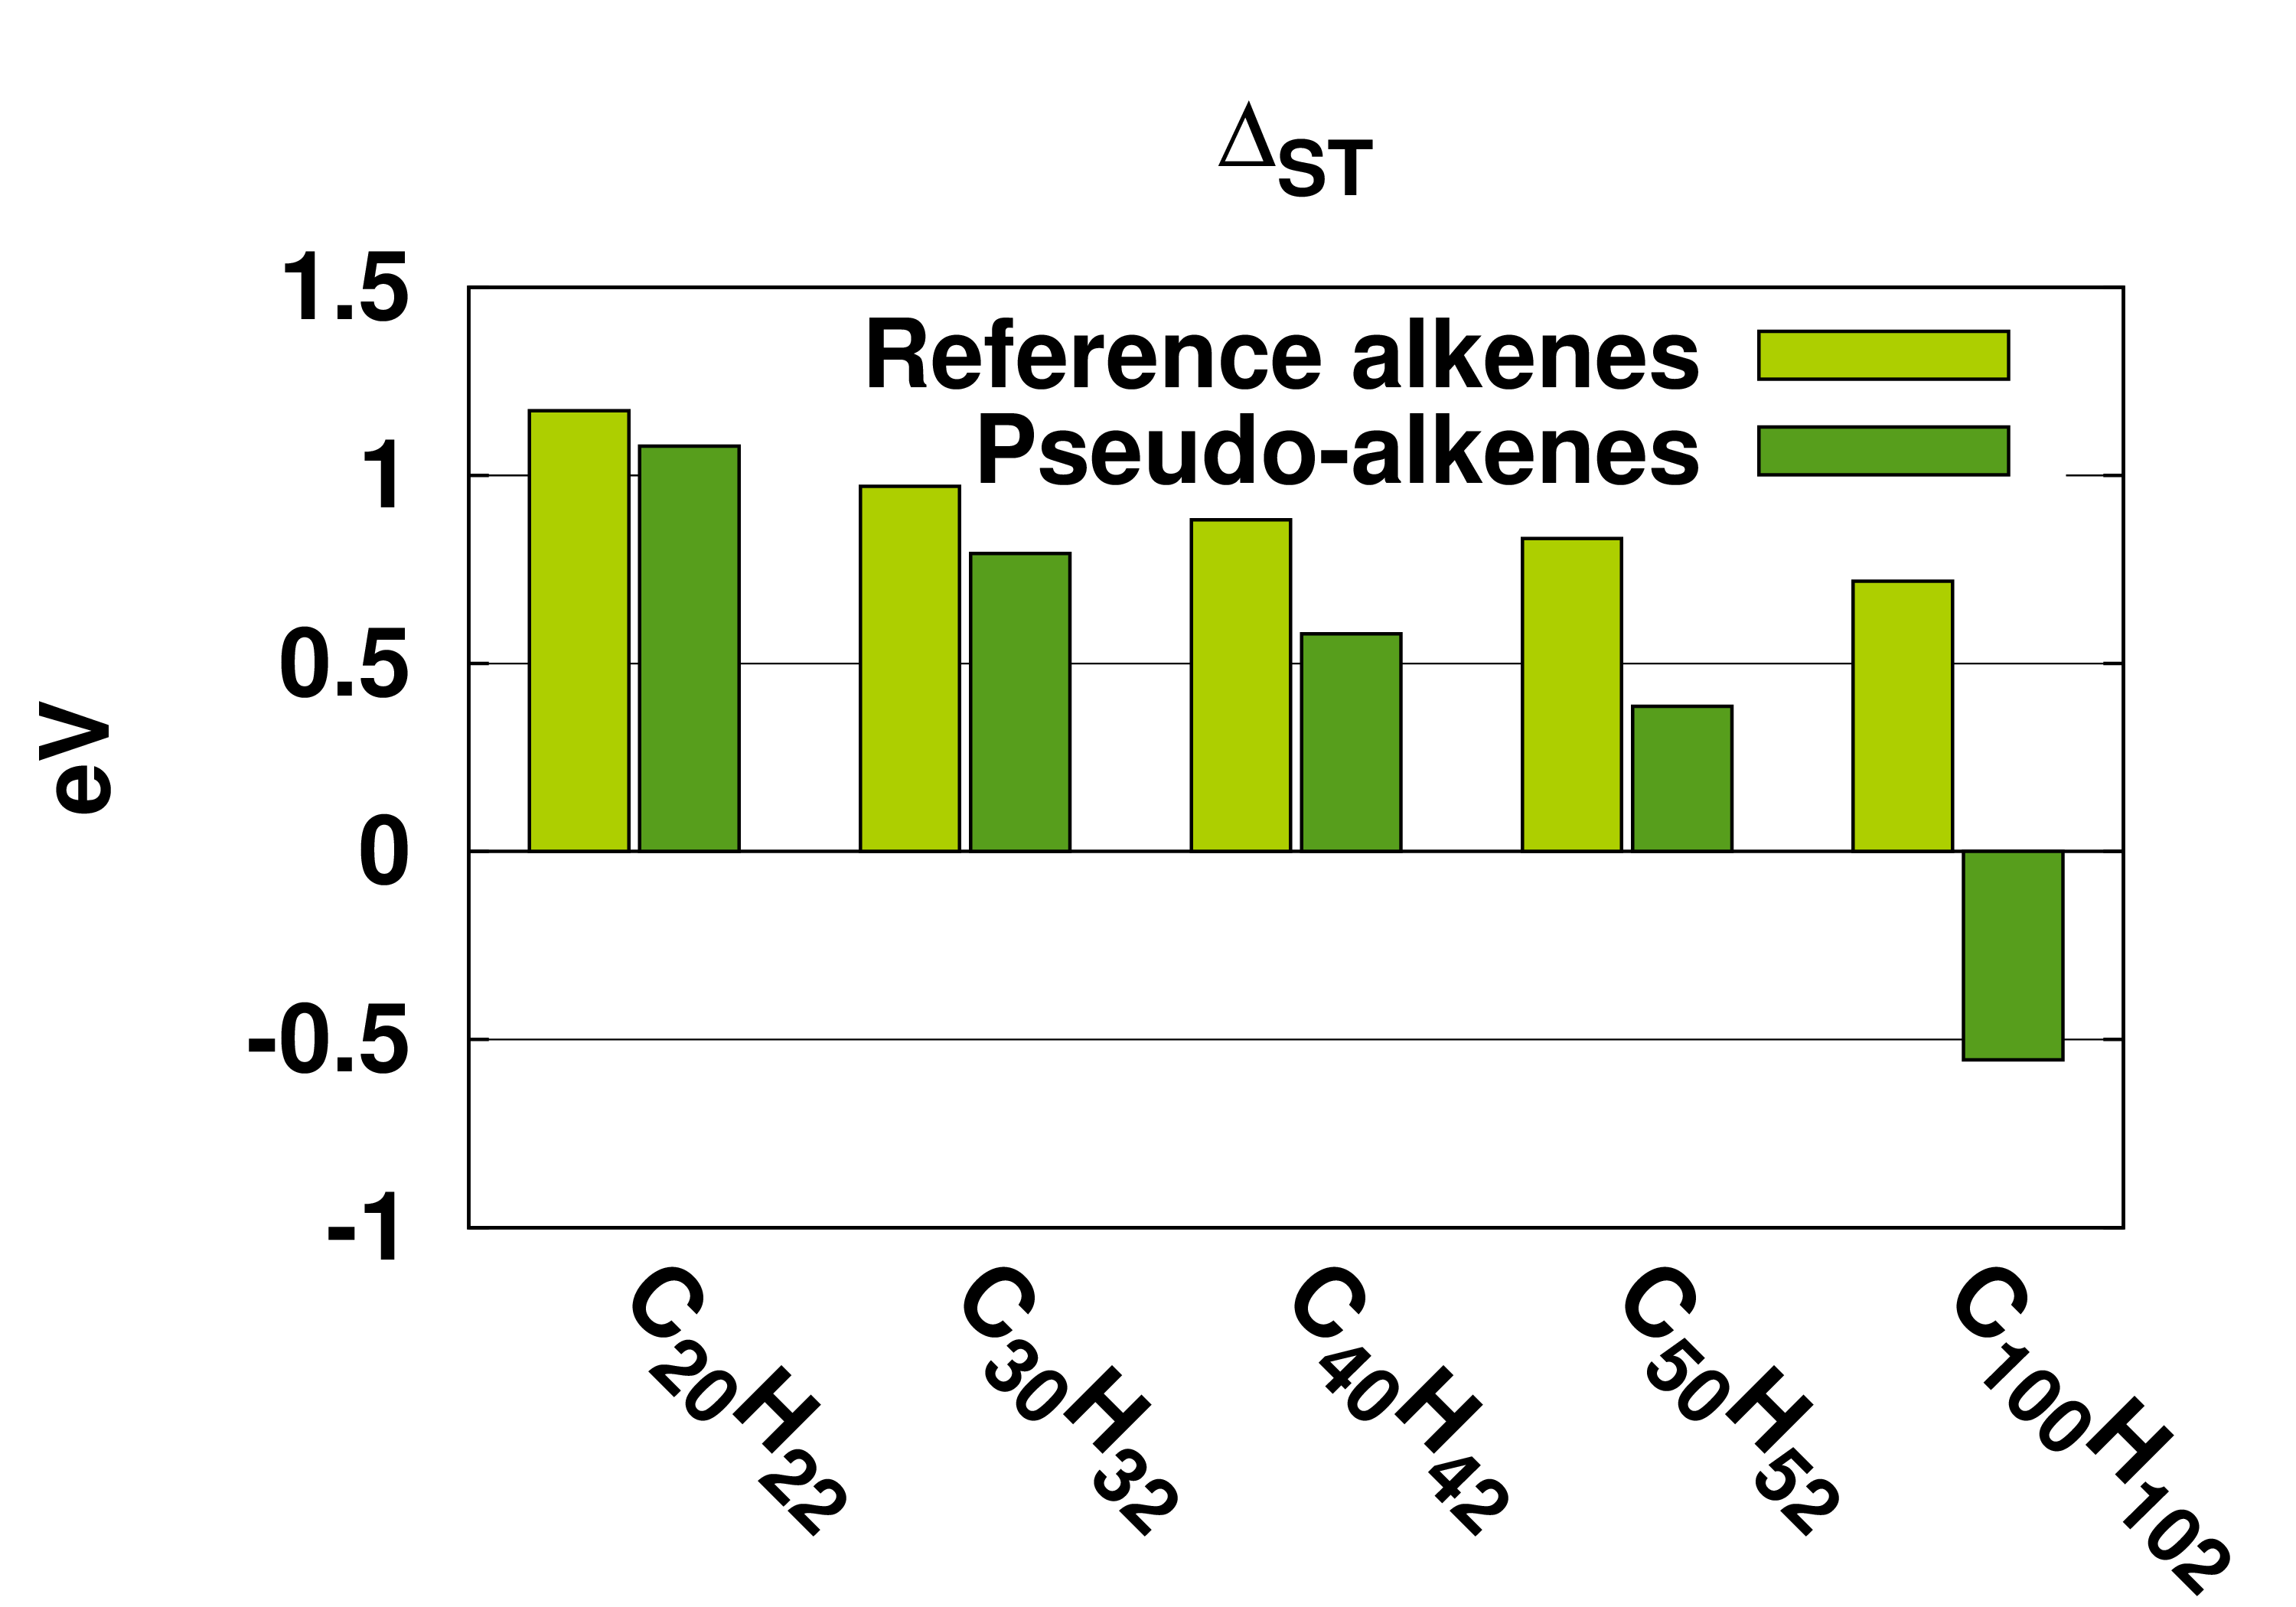
\includegraphics[width=8cm]{long_pbe0_st}
% FIGURES 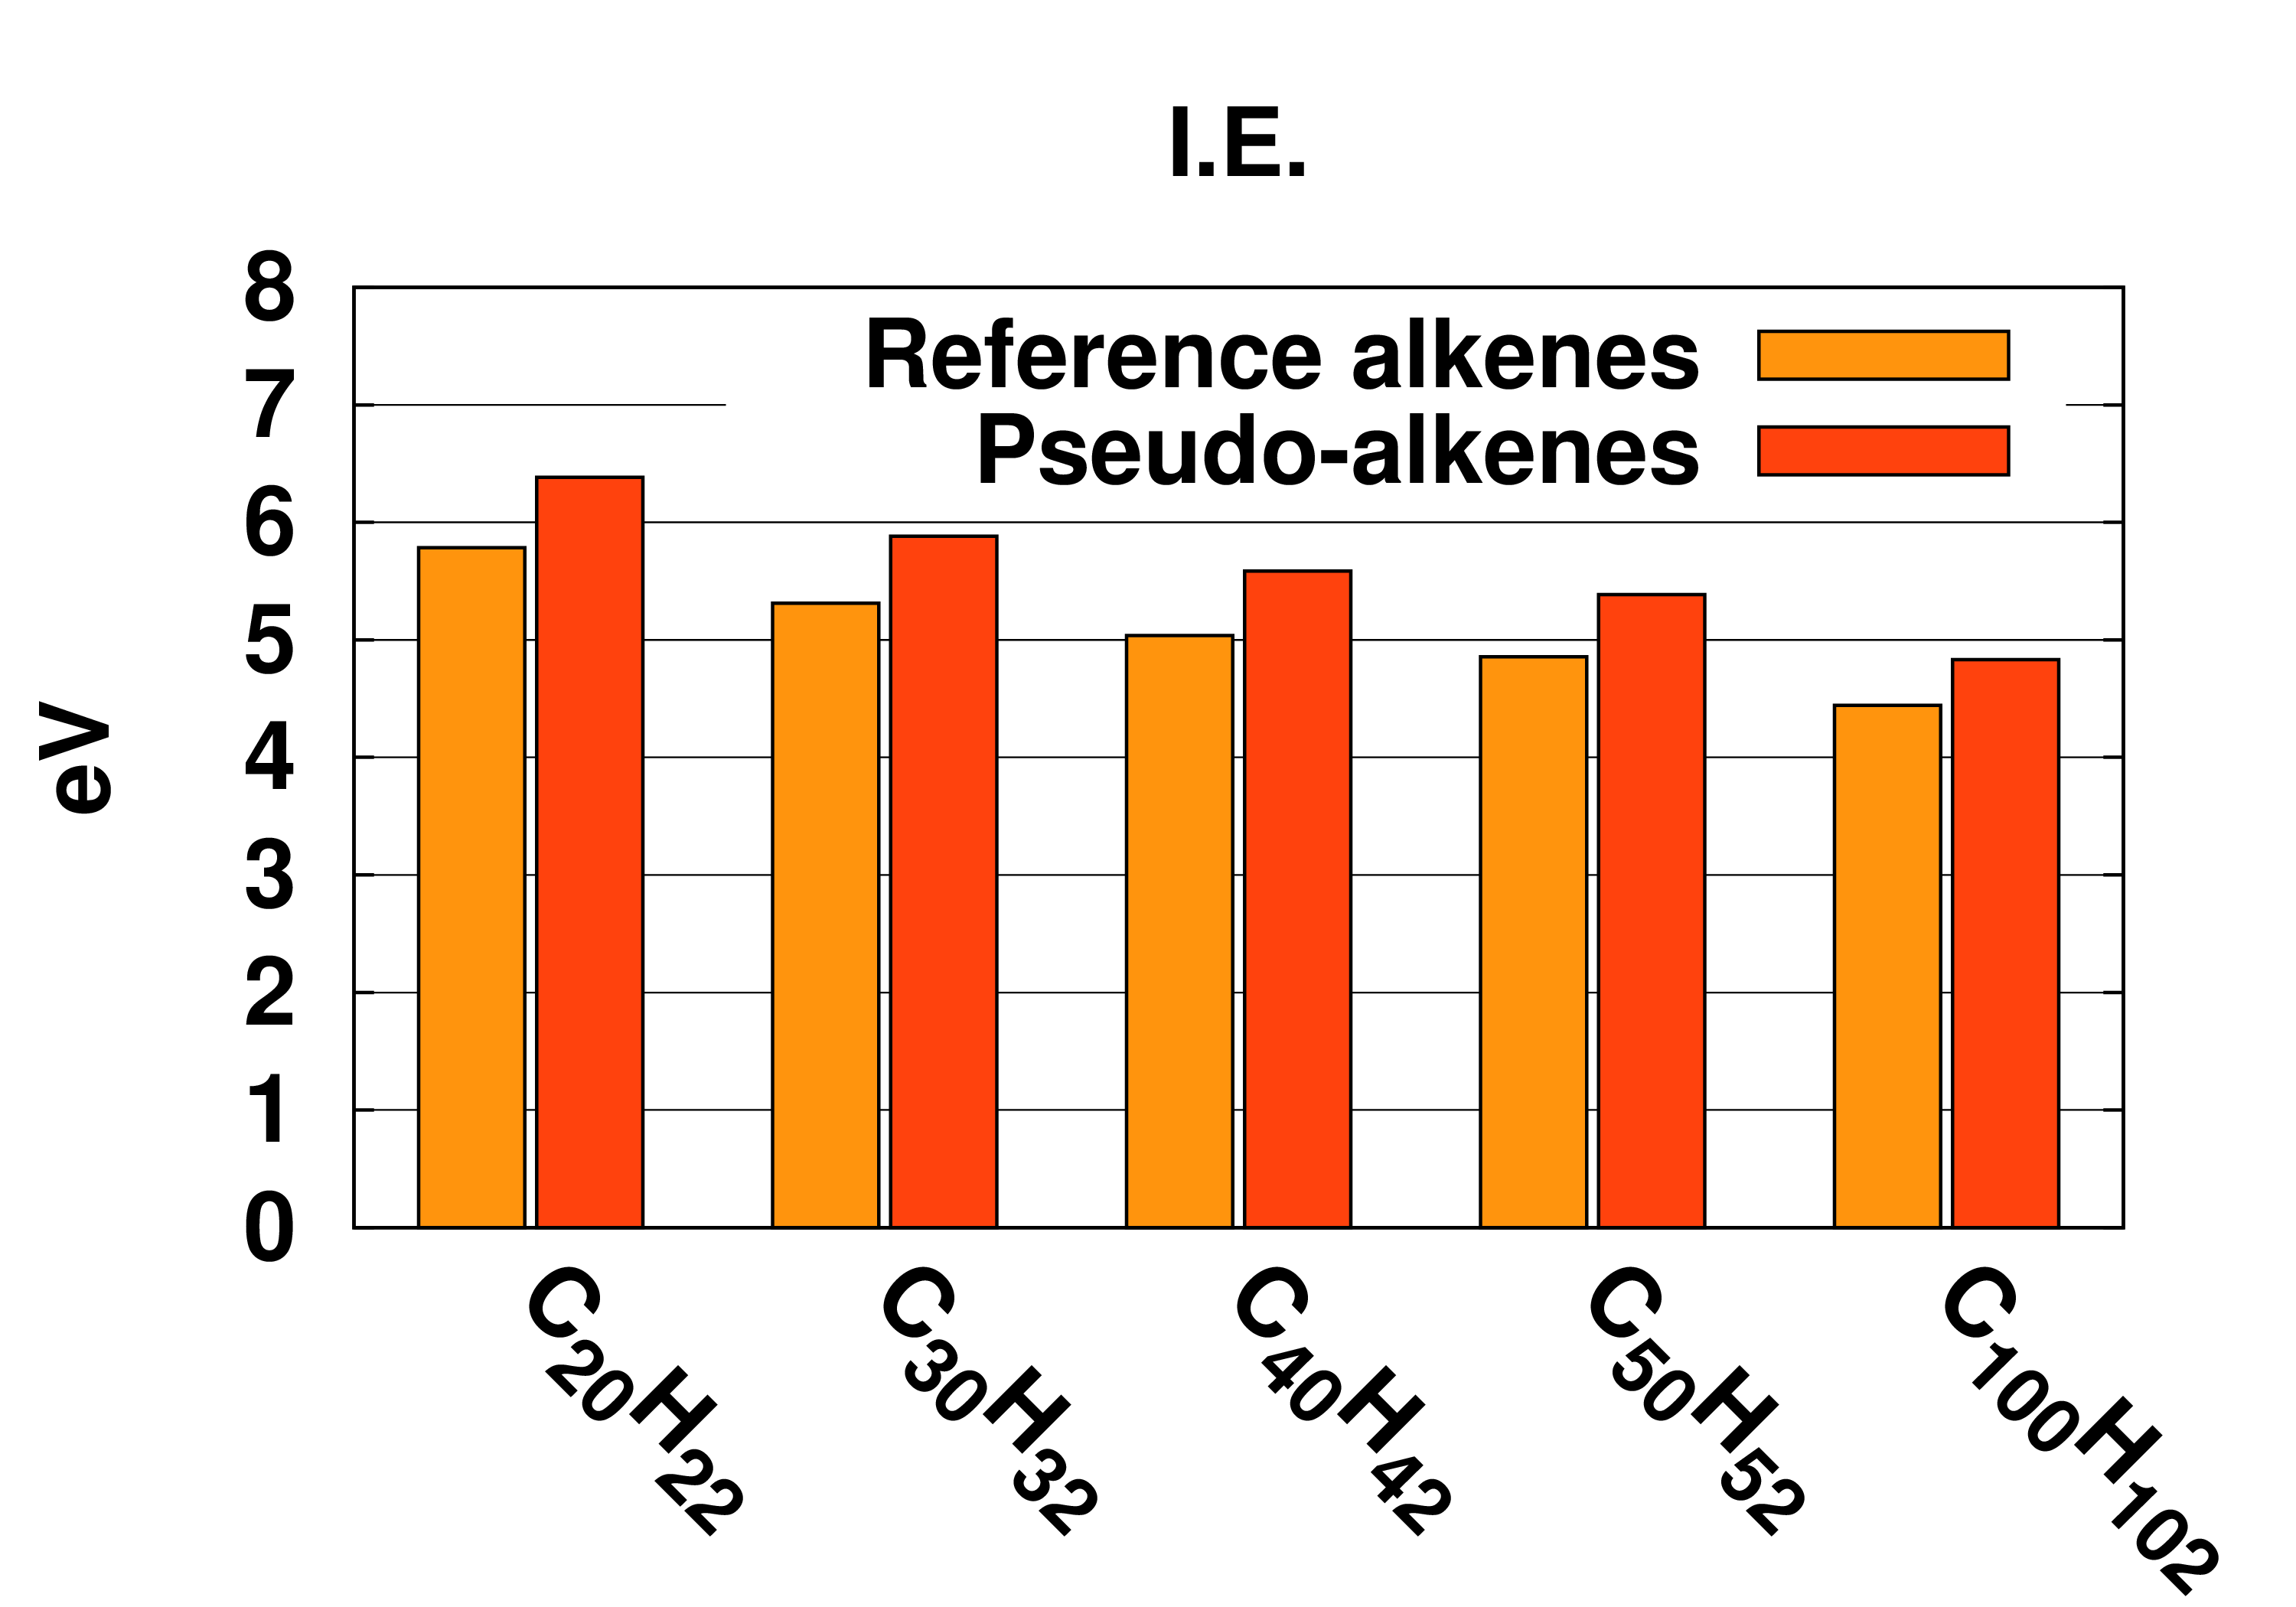
\includegraphics[width=8cm]{long_pbe0_ie}
% FIGURES 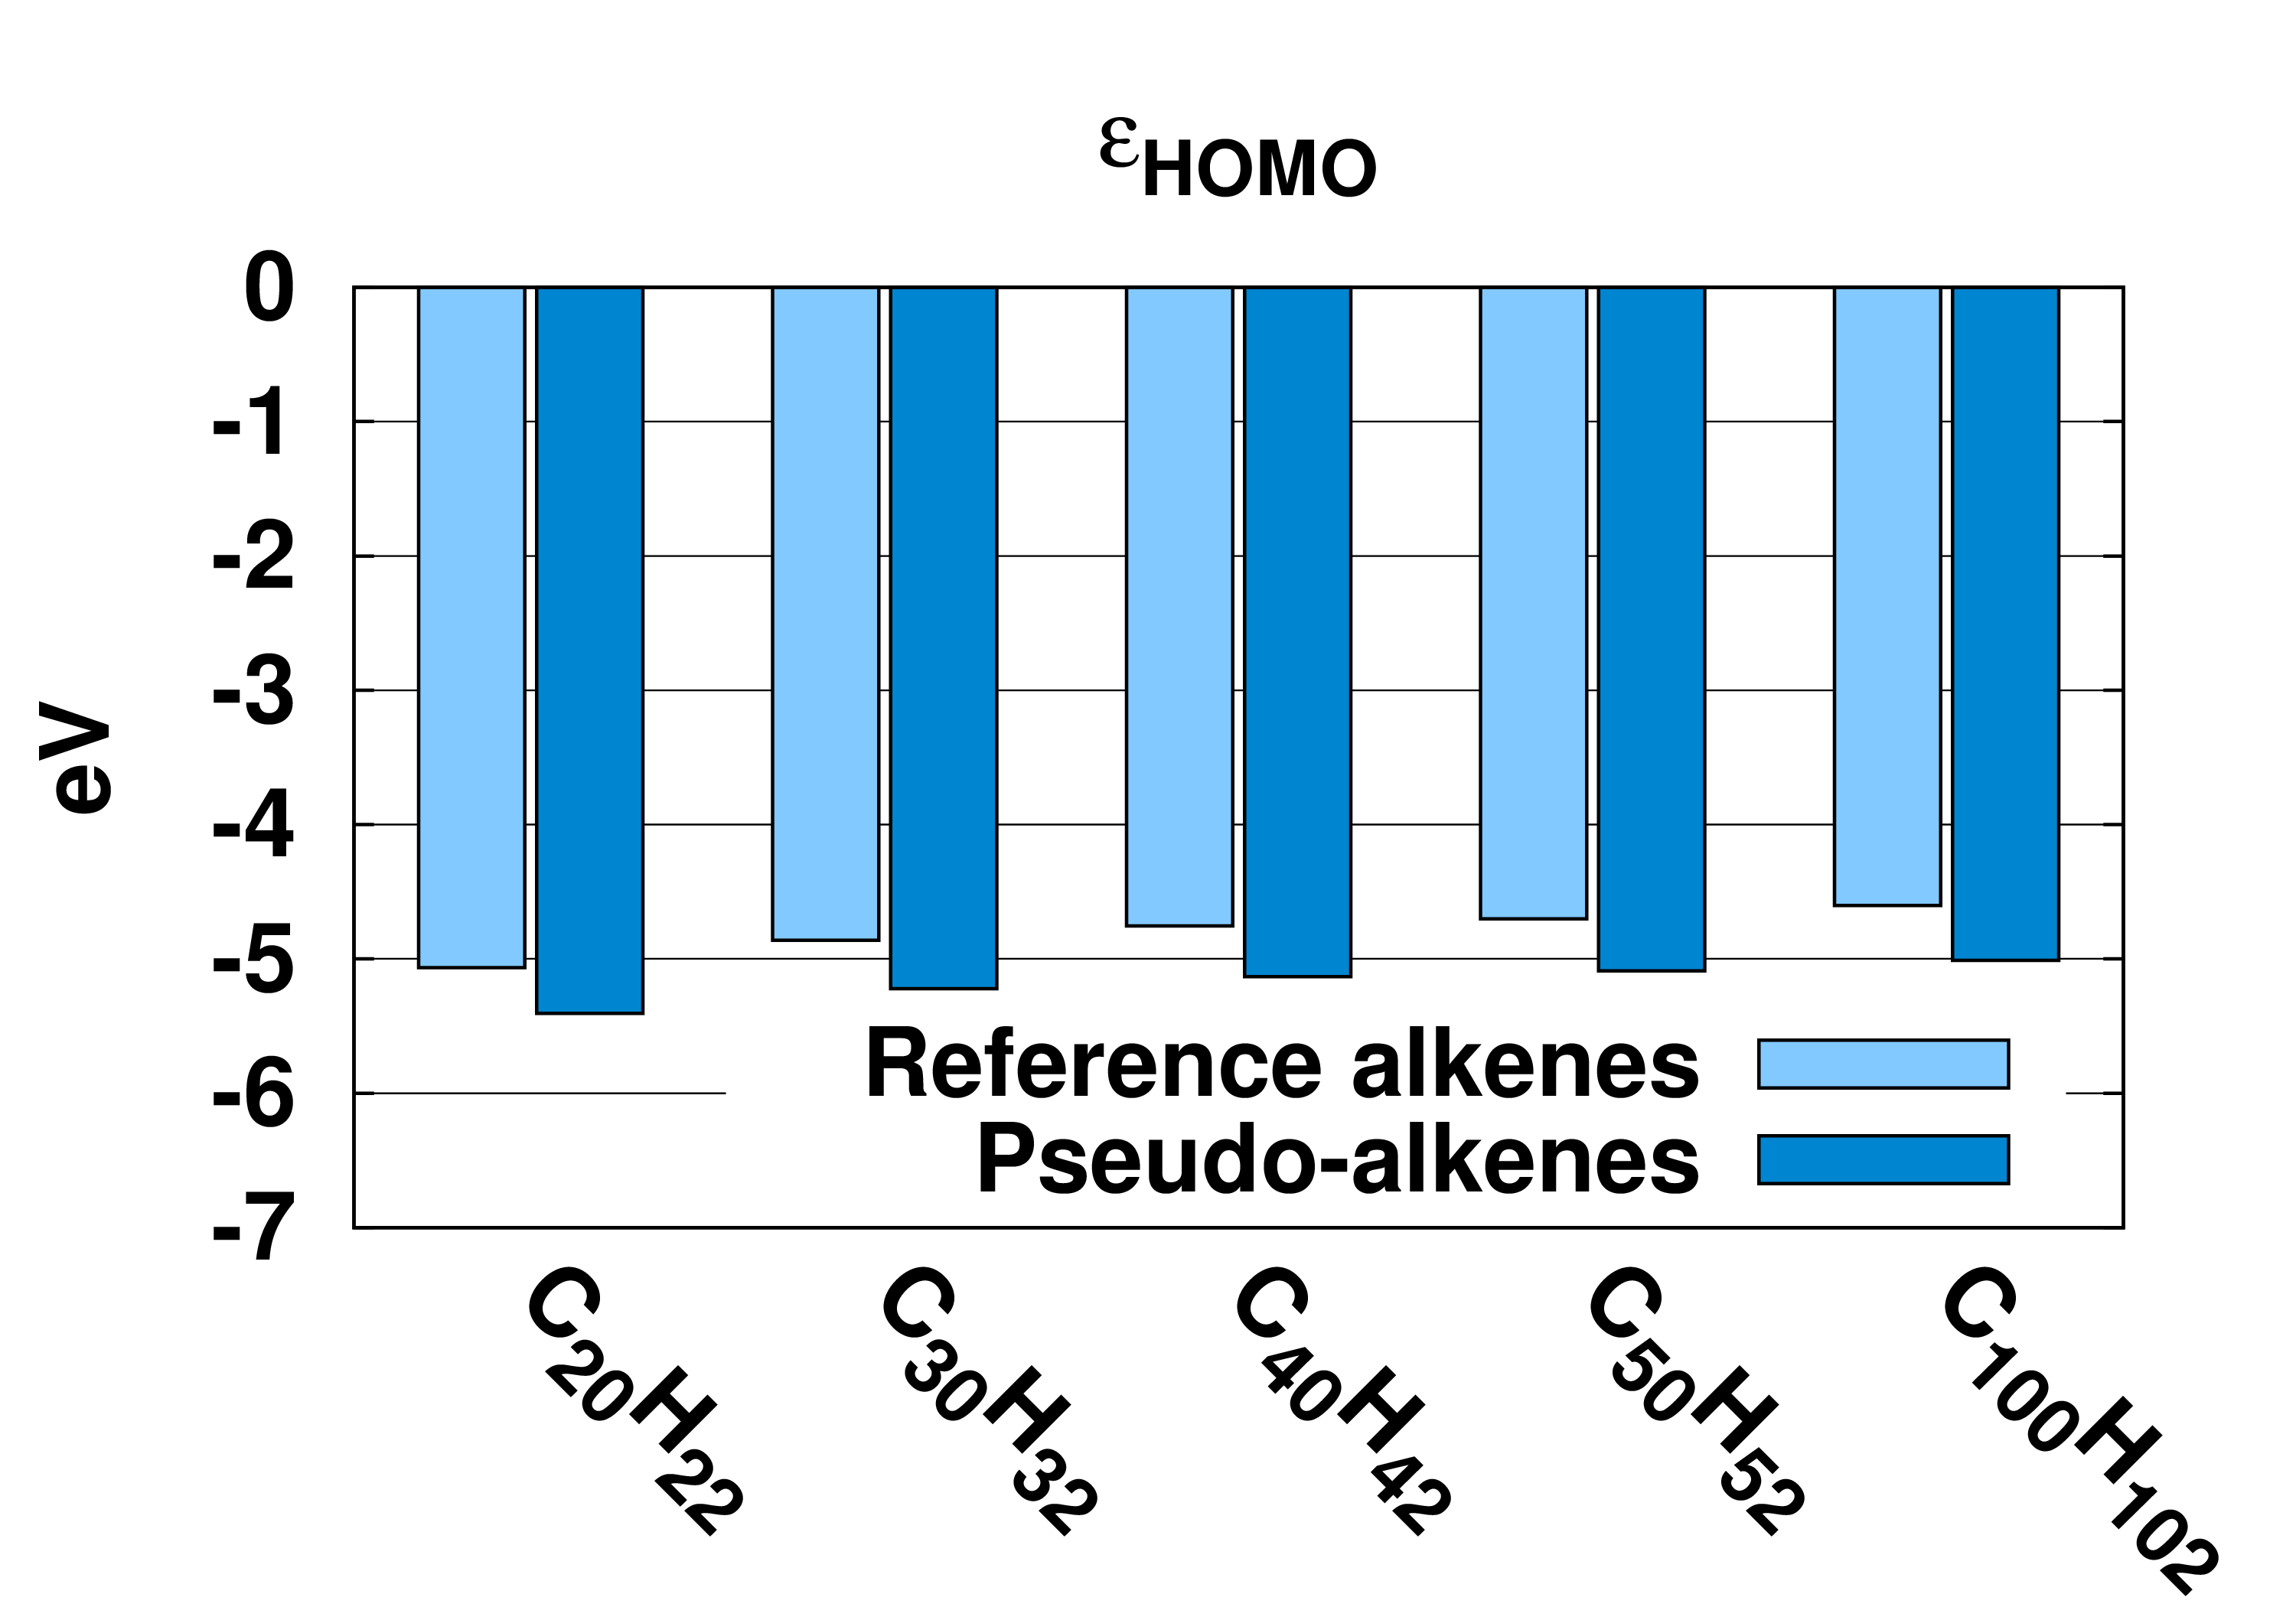
\includegraphics[width=8cm]{long_pbe0_homo}
% FIGURES 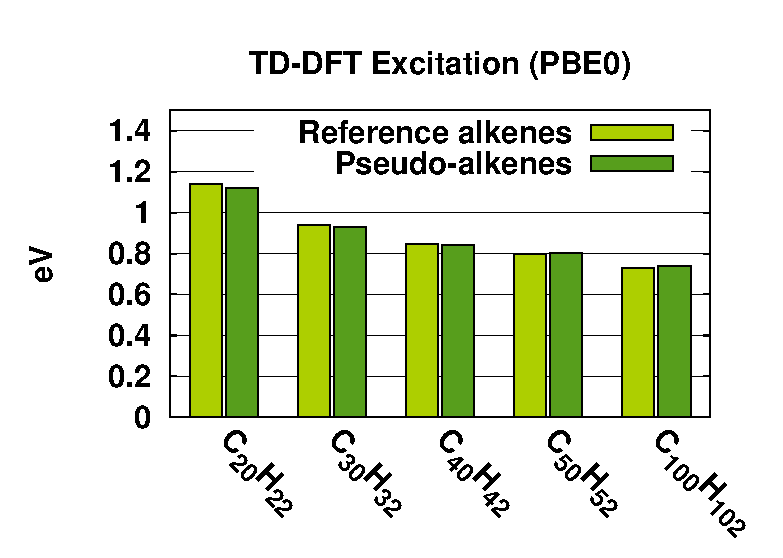
\includegraphics[width=8cm]{long_pbe0_tddft}
% FIGURES %\caption{DFT and TD-DFT (PBE0) comparison of reference and pseudo-system energies across a range of long chain alkenes (C\(_{20}\)-C\(_{100}\)).}
% FIGURES %\label{fig:long_chain_graphs}
% FIGURES \end{center}
% FIGURES \vspace{0.25in}
% FIGURES \hspace*{3in}
% FIGURES {\Large
% FIGURES \begin{minipage}[t]{3in}
% FIGURES \baselineskip = .5\baselineskip
% FIGURES Figure 6 \\
% FIGURES Alexander Punter, Paola Nava, Yannick Carissan \\
% FIGURES J.\ Comput.\ Chem.
% FIGURES \end{minipage}
% FIGURES }
% FIGURES 
% FIGURES \clearpage
% FIGURES 
% FIGURES %\vspace*{0.1in}   %%% FIGURE 7
% FIGURES \begin{center}
% FIGURES 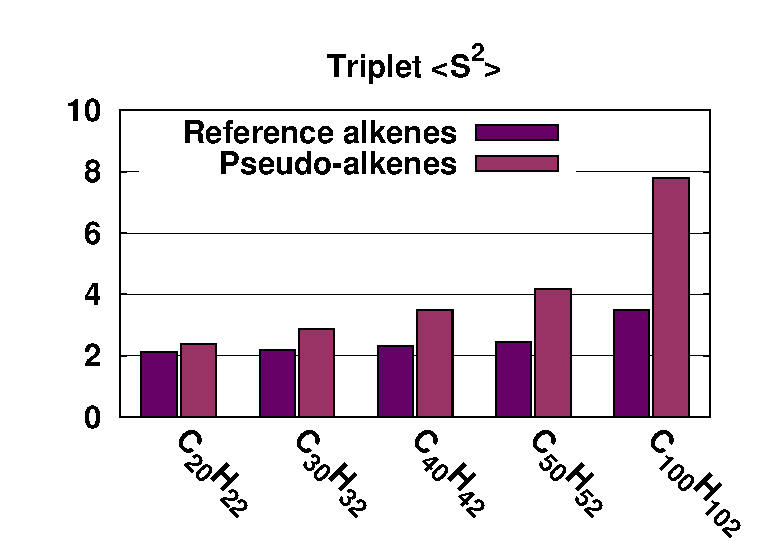
\includegraphics[width=8cm]{long_pbe0_s2}
% FIGURES %\caption{Comparison of $S^2$ expectation values obtained for the calculation
% FIGURES %of the first triplet configuration in a SCF formalism, for reference
% FIGURES %and pseudo-systems.}
% FIGURES %\label{fig:ssquare}
% FIGURES \end{center}
% FIGURES \vspace{0.25in}
% FIGURES \hspace*{3in}
% FIGURES {\Large
% FIGURES \begin{minipage}[t]{3in}
% FIGURES \baselineskip = .5\baselineskip
% FIGURES Figure 7 \\
% FIGURES Alexander Punter, Paola Nava, Yannick Carissan \\
% FIGURES J.\ Comput.\ Chem.
% FIGURES \end{minipage}
% FIGURES }
% FIGURES 
\clearpage
%ENDFIG
%BEGTAB

%\begin{table}
%\begin{tabular}{|c|c|c|c|}\hline
%\textbf{Quantity} & \textbf{Calculated} & \textbf{Observed} & \textbf{Error} \\ \hline
%  Density & 5.3 & 6.3 & Within limits \\ \hline
%  Optical magnification & 8.3 & 90.9 & Utterly unacceptable\! \\ \hline
%\end{tabular}
%\caption{\label{tbl1} Place table caption here.}
%\end{table}

\begin{table}[ht]
\begin{tabular}{c c c}
\hline
 & Coefficient & Exponent \\ 
\hline
HF & -2.594 & 1.0 \\
 & -4.788 & 5.0 \\
 & -7.524 & 10.0 \\
\hline
PBE0 & -2.605 & 1.0 \\
 & -4.873 & 5.0 \\
 & -7.678 & 10.0 \\
\hline
\end{tabular}
\caption{Coefficients and exponents for \(s\)-only pseudo-potentials for CH\(^{\bullet}_{3}\), optimised to give 
the all-electron HOMO reference energy of  -10.537~eV (HF) and -6.726~eV (PBE0). 
\(d = 0.5\) a.u., as defined in Figure~\ref{figure:ref_pseudo_diagram}.}
\label{table:ch3_s_potentials}
\end{table}

\newpage

\begin{table}[ht]
\begin{tabular}{c c c c}
\hline
& $d$ & \(s\) coefficient & \( \pi \)  \\
\hline
HF$^a$   &     &        & -10.363 \\
PBE0$^a$ &     &        & -6.632 \\
HF       & 2.0 & -7.521 & -9597.0 \\
HF       & 0.5 & -7.521  & -7.905 \\
PBE0     & 0.5 &-7.678  & -8.447 \\
\hline
\multicolumn{4}{l}{$^a$ All-electron reference values.}\\
\end{tabular}
\caption{HOMO energies ($\pi$, eV) for ethene and pseudo-ethene. The pseudo-potentials used in the pseudo-ethene are taken from optimised values for 
pseudo-CH\(^{\bullet}_{3}\) with only \(s\)-potentials and an exponent of 10.0. $d$ (a.u.) as defined 
in Figure~\ref{figure:ref_pseudo_diagram}.}
\label{table:ethene_s_pseudo}
\end{table}

\newpage

\begin{table}[ht]
\begin{tabular}{c c c c}
\hline
& \(p\) coefficient & \(p\) exponent \\
\hline
\(p_{z}\) potential & -3.267 & 0.295 \\
\hline
Calculation Type & \(s\) coefficient & \(s\) exponent & \(\pi\) \\
\hline
HF & 2.772 & 1.0 & -13.654 \\
 & 6.173 & 5.0 & -14.011 \\
 & 10.381 & 10.0 & -14.061 \\
\hline
PBE0 & 3.483 & 1.0 & -10.325 \\
 & 9.801 & 5.0 & -10.409 \\
 & 18.351 & 10.0 & -12.543 \\
\hline
\end{tabular}
\caption{\(\pi\) orbital energy values (eV) for pseudo-ethene, using \(s\) and \(p\) pseudo-potentials.
The pseudo-potentials are taken from a pseudo-CH\(^{\bullet}_{3}\) system optimised to give the correct all-electron HOMO energy.}
\label{table:p_potentials}
\end{table}

\newpage

\begin{table}[ht]
\begin{tabular}{c c c c c}
\hline
\(s\) coefficient & \(s\) exponent & $\Delta_{ST}$  & Ionisation  & $\varepsilon_{HOMO}$  \\
\hline
\multicolumn{2}{c}{\textit{Reference Values}} & -3.533 & -9.091 & -10.363 \\
\hline
&& \multicolumn{3}{l}{\(p\) coefficient -3.267; \(p\) exponent 0.295} \\
\hline
0.552 & 0.1 & -3.533 & -27.158 & -27.31 \\
0.608 & 1.0 & -3.533 & -28.247 & -28.395 \\
0.936 & 5.0 & -3.533 & -29.583 & -29.722 \\
\hline
\multicolumn{2}{c}{\textit{Optimal Values}} &\multicolumn{3}{l}{\(p\) coefficient -3.91; \(p\) exponent 0.624} \\
\hline
1.5 & 0.5 & -3.533 & -9.806 & -10.062 \\
\hline
\end{tabular}
\caption{\(s\)-potential fits to ethene properties as defined in the text (eV). All values are from HF calculations, and \(d = 0.5\) a.u.}
\label{table:ethene_excitations}
\end{table}

\newpage

\begin{table}[h]
\begin{tabular}{c c c c c c }
\hline
Calculation Type & HF & PBE0 & PBE & TPSS & TPSSh \\
\hline
Mean \(\pi - \pi*\) Triplet-Singlet error (\%) & 4.1 & 3.6 & 7.5 & 13.3 & 11.4 \\
Mean Ionisation error (\%) & 5.3 & 6.0 & 8.1 & 10.1 & 9.0 \\
Mean Singlet HOMO error (\%) & 1.3 & 4.0 & 8.5 & 12.0 & 9.7 \\
Mean TD-DFT Excitation error (\%) & - & 2.6 & - & - & - \\ 
\hline
\end{tabular}
\caption{\%-errors across calculation types for short chain alkenes  (C\(_{2}\)-C\(_{12}\))}
\label{table:alkene_errors}
\end{table}

\newpage

\begin{table}[h]
\begin{tabular}{c c c c c c }
\hline
Calculation Type & HF & PBE0 & PBE & TPSS & TPSSH \\
\hline
Mean \(\pi - \pi*\) Triplet-Singlet error (\%) & 3.3 & 1.9 & 1.7 & 6.8 & 6.7 \\
Mean Ionisation error (\%) & 7.4 & 10.0 & 12.5 & 14.4 & 13.0 \\
Mean Singlet HOMO error (\%) & 3.4  & 9.3  & 13.4 & 17.1 & 14.7 \\
Mean TD-DFT Excitation error (\%) & - & 0.099 & - & - & - \\ 
\hline
\end{tabular}
\caption{\%-errors across calculation types for ring-systems}
\label{table:ring_system_errors}
\end{table}

\newpage

\begin{table}[h]
\begin{tabular}{c c c c c c }
\hline
Calculation Type & HF & PBE0 & PBE & TPSS & TPSSH \\
\hline
Mean \(\pi - \pi*\) Triplet-Singlet error (\%) & 55.3 & 85.8 & 83.4 & 239.8 & 320.2 \\
Mean Ionisation error (\%) & 25.1 & 6.7 & 9.4 & 10.3 & 11.6 \\
Mean Singlet HOMO error (\%) & 1.8 & 7.3 & 11.3 & 16.7 & 13.6 \\
Mean TD-DFT Excitation error (\%) & - & 0.005 & - & - & - \\ 
\hline
\end{tabular}
\caption{\%-errors across calculation types for long chain alkenes (C\(_{20}\)-C\(_{100}\))}
\label{table:long_alkene_errors}
\end{table}

\newpage

\begin{table}
\begin{tabular}{c c c c}
\hline
\multicolumn{2}{c}{Excitation} & \multicolumn{2}{c}{Weight(\%)}\\
\multicolumn{2}{c}{MO} & Ref. & Pseudo.\\
\hline
\multicolumn{2}{c}{25 a" \(\rightarrow\) 26 a"} & 77.0 &   67.1  \\
\multicolumn{2}{c}{24 a" \(\rightarrow\) 27 a"} & 10.5 &   13.1  \\
\multicolumn{2}{c}{23 a" \(\rightarrow\) 28 a"} & 3.6  &    5.2  \\
\hline
\end{tabular}
\caption{\label{tab:coef}Comparison of the weights (all electron \emph{vs.} pseudo-potentials)
of the excitations obtained with TD-DFT
to represent the triplet excited state from the closed shell singlet state.
Example case of C$_{50}$H$_{52}$.}
\end{table}
%ENDTAB

\end{document}

